% IMPORTANT NOTE: I've never dealt much with syntax before, at least not in a
% way as formal as I'm trying to come to terms with it here. If there's
% anything wrong with my analyses, it's because I don't know enough yet. Things
% may be subject to change *especially* in this chapter.

\chapter{Syntactic typology}
\label{ch:syntyp}
\index{typology|(}

While the previous chapter dealt largely with the various parts of speech and
their inflectional properties, the present chapter and the next will elaborate
on how these words combine into syntactic phrases.\footnote{Since trees and
tableaus are large, many regularly numbered examples in the following will
appear not in place, but floated. Furthermore, note that this is my first time
learning more about formal syntax, and trying to apply it. Thus, I do not claim
for the present analyses to be complete or flawless; they are merely first
steps.} Since Ayeri is a verb-initial language\index{word order}, it is probably rather
comfortably analyzed in terms of Lexical-Functional Grammar
(\cite{bresnan1982}~ff.; more recently, \cite{bresnan2016};
\cite{dalrymple2001}; \cite{falk2001}), since
\Lfg{}\index{Lexical-functional grammar} does not require complicated derivations behind the surface structure of
sentences.\footnote{Passivization, for instance, is assumed to be a lexically
motivated alternation in predicate structure (\Subj{} is blocked, so the
nominative is assigned to \Obj{}, and the original \Subj{} is expressed by an
\Oblq{agt}), rather than an internal derivational process
\citep[23\psqq]{bresnan2016}.} It will be assumed here that, even though Ayeri's
unmarked word order\index{word order} is VSO with predicate and predication not
adjacent to each other, it is configurational\index{configurationality} in that there is
a VP\index{phrase types!verb phrase} which c-commands a number of other constituents as complements and
adjuncts in transitive sentences\index{verbs!transitive}.

\section{Lexical-functional grammar}
\index{Lexical-functional grammar|(}

In principle, \Lfg{} assumes that grammar operates on different structural
levels in parallel: mainly, these are a(rgument) structure, c(onstituent)
structure, and f(unctional) structure; other layers have been proposed by
different researchers for different purposes \citep[862--865]{buttking2015}.
\citet{bresnan2016} define three core design principles for \Lfg{}:

\begin{description}
\item[Variability:] \textcquote[41]{bresnan2016}{The principle of variability
states that \emph{external structures vary across languages}. The formal model
of external structure in \Lfg{} is the \emph{c-structure}, which stands for
\enquote{constituent structure} or \enquote{categorial structure}}. 
C-structures are commonly represented by context-free phrase-structure rules;
constituency trees are based on an extended version of X-bar theory\index{X-bar
theory} \citep[42]{bresnan2016}.\footnote{The basic recursive rules of X-bar
theory\index{X-bar theory} are observed:
\begin{enumerate}[nosep, leftmargin={2\footnotemargin}]
\item XP → YP, \xbar{X} (specifier rule)
\item \xbar{X} → \xbar{X}, ZP (adjunct rule)
\item \xbar{X} → \xhead{X}, WP (complement rule)
\end{enumerate}

The principle of economy of expression furthermore dictates that essentially,
trees be pruned of empty terminal nodes and non-branching preterminal nodes,
since these do not provide structurally or semantically relevant information
\citep[119--128]{bresnan2016}. Thus, for instance, in a rule like XP →
\xhead{X} YP, YP does not necesssarily appear as XP's complement in the tree if
one were to follow plain X-bar theory\index{X-bar theory} rules. Rather, nodes
are defined in their status by functional annotations than by their position in
the tree alone.}

\item[Universality:] \textcquote[42]{bresnan2016}{The principle of universality
states that \emph{internal structures are largely invariant across languages}.
The formal model of internal structure in \Lfg{} is the \emph{f-structure},
which stands for \enquote{functional structure}}. The f-structure is depicted
as an argument-value matrix (\Avm{}) which maps the relations between `subject'
(\Subj{}), `object' (\Obj{}), `predicator' (\Pred{}), etc.\ as functional
abstractions of NP, VP, \xhead{V}, etc.\ \citep[42]{bresnan2016}.
Complement-taking predicators, such as verbs or adpositions, are also presented
with their \fw{a-structure} spelled out. That is, subcategorized-for arguments
are formally stated \citep[15]{bresnan2016}. The f-structure collates semantic
features associated with heads of grammatical functions (\GF{}s), such as case
(\Case{}), person (\Pers{}), number (\Num{}), which are abstract features and
need not have morphological realization \citep[43]{bresnan2016}.

\item[Monotonicity:] \textcquote[43]{bresnan2016}{Constituent structure form is
simply not the same in all languages [...]\ In \Lfg{} the correspondence
mapping between internal and external structures does not preserve sameness of
form. Instead, \emph{it is designed to preserve inclusion relations between the
information expressed by the external structure and the content of the internal
structure}}. Due to the monorepresentation principle, information distributed
over different morphemes which logically belongs to a single grammatical
function is unified in f-structure.

\end{description}

\begin{figure}[t]\centering
\begin{tabular}[t]{l @{\quad\quad} c}
argument (a-)structure:
& \astruct{\tikzmark{verb}verb}{\tikzmark{x}x, \tikzmark{y}y}\bigskip \\

functional (f-)strucutre:
& \tikzmark{fstruct}{\smaller\begin{avm}
\[
	\quad \Subj{} \tikzmark{subj} & \[
		{\enspace}\vdots{\enspace} \\
	\]{\quad} \\
	\quad \Obj{} \tikzmark{obj} & \[
		{\enspace}\vdots{\enspace} \\
	\] \tikzmark{objval}{\quad} \\
	\quad \tikzmark{pred} \Pred{} & \dots \tikzmark{predval} \\
\]
\end{avm}}\bigskip\\

constituent (c-)structure:
& \begin{forest} baseline
[\xbar{V}
	[\subnode{V}{V}]
	[NP \tikzmark{NP}
		[\xbar{N} \tikzmark{Nbar}]
	]
]
\end{forest}
%
\end{tabular}
\begin{tikzpicture}[remember picture, overlay]
\draw [-latex]
	([xshift=1.5ex, yshift=-0.5ex]{pic cs:verb})
	to [out=south, in=north west]
	([yshift=1ex]{pic cs:pred});
\draw [-latex]
	([xshift=0.5ex, yshift=-0.5ex]{pic cs:x})
	to [out=south, in=north east]
	([yshift=1ex]{pic cs:subj});
\draw [-latex]
	([xshift=0.5ex, yshift=-0.75ex]{pic cs:y})
	to [out=south, in=north east]
	([yshift=1ex]{pic cs:obj});
\draw [-latex]
	([yshift=1ex]{pic cs:V})
	to [out=west, in=south west]
	([yshift=-10ex]{pic cs:fstruct});
\draw [-latex]
	([yshift=1ex]{pic cs:NP})
	to [out=east, in=east]
	([yshift=1ex]{pic cs:objval});
\draw [-latex]
	([yshift=1ex]{pic cs:Nbar})
	to [out=east, in=east]
	([yshift=1ex]{pic cs:objval});
\end{tikzpicture}
\caption[F-structure mappings]{F-structure mappings \citep[15]{bresnan2016}}
\label{fig:phimap}
\end{figure}

To illustrate the different parallel structures in operation,
\citet[15]{bresnan2016} give the schema in \autoref{fig:phimap} to demonstrate
which part of the a- and c-structure respectively corresponds (`links', `maps')
to which part of the f-structure.
% \footnote{\citet{bresnan2016} use \textsc{`subj'} for `subject'. ; for
% consistency with the above I will use `\Subj{}' in the following. I will also
% divergently use \Compl{} and \XCompl{} for \textsc{(x)comp}, since
% \textsc{comp} has already been used for `comparative' above.}
Regarding the different functions distinguished, \Lfg{} assumes the functional
hierarchies given in (\ref{ex:functions}) of \autoref{ch:syntyp}, following
\citet[97, 100]{bresnan2016}.

\begin{figure}[h]
\pex\label{ex:functions}
\a\label{ex:gfs} Grammatical functions (\GF{}s):\\
	$\overbrace{\Subj{} > \Obj{} > \SObj{}}^{\text{core}} > 
	\overbrace{\Oblique{} > \XCompl{}, \Compl{} > \Adjc{}}^{\text{noncore}}$

\a\label{ex:nonafs} (Non-)argument functions (\AF{}s/$\overline{\mbox{\AF{}}%
}$s):\\
	$\underbrace{\Top{}\: \Foc{}}_{\text{non-a-fns}}\; 
	\overbrace{\Subj{}\: \Obj{}\: \SObj{}\: \Oblique{}\: \XCompl{}\: 
		\Compl{}}^{\text{a-fns}}\; 
	\underbrace{\Adjc{}}_{\text{non-a-fns}}$

\a\label{ex:dfs} Discourse functions (\DF{}s):\\
	$\overbrace{\Top{}\: \Foc{}\: \Subj{}}^{\text{d-fns}}\;
	\underbrace{\Obj{}\: \SObj{}\: \Oblique{}\: \XCompl{}\: \Compl{}\: 
		\Adjc{}}_{\text{non-d-fns}}$
\xe
\end{figure}

The functions listed in (\ref{ex:functions}) will also appear in
phrase-structure rules and c-structure trees together with arrows. These arrows
symbolize inheritance of feature information from the current level (↓) of the
tree to the next (↑), so for instance, `\pass{\Subj}' means that the
information subsumed by the current node (`down') is passed on as part of the
subject function of the next higher level (`up') in the tree. Concise
information on notational formalisms of \Lfg{} can be found, for instance, in
\citet{buttking2015}.

\index{Lexical-functional grammar|)}

\section{Typological considerations}
\label{sec:verbtypo}

Verbs govern the relations of the various phrase types to each other and they
are thus central to the formation of clauses. Just from looking at the numerous
examples in the previous section, it should have become clear that Ayeri's
preferred word order is verb-first, which opens up a few typological
questions---first and foremost, whether Ayeri actually has a verb phrase, or in
terms of generative grammar: whether it is configurational. As we have seen,
Ayeri definitely has a constituent structure as far as NPs, APs, PPs, etc. are
concerned. However, due to VSO word order, it is not obvious whether verb and
object actually form a VP constituent together, since V and O are not adjacent
to each other. Since Ayeri marks topics in terms of morphology, it will also be
necessary to discuss how this mechanism works and how it relates to the notion
of the subject.

A discussion of subject, topic, and configurationality is interesting also in
that Ayeri's syntactic alignment was originally \emph{inspired} by the
Austronesian, or Philippine, alignment system. Tagalog, an Austronesian
language of the Malayo-Polynesian branch, spoken mainly in the Philippines
\parencites{glottolog:tgl}{schachterotanes1972}, usually serves as the
academic poster child in descriptions of this system. Ayeri departs from
Tagalog's system in a number of ways, though, and very probably towards the
more conventional. Austronesian alignment is thus not necessarily the best
model to liken Ayeri's syntax to. It will nonetheless be informative to compare
both systems based on the work of \textcites{kroeger1991}{kroeger1993a}, who
provides an analysis of Tagalog's syntactic alignment at least roughly in terms
of the \Lfg{} framework and describes some heuristics which may be helpful in
establishing what is actually going on in Ayeri.\footnote{As mentioned in the
introductory chapter, I started Ayeri in late 2003---then still in high school
and not knowing much about linguistics. Of course, I had to go and pick as a
model the one alignment system which has long been \textquote{a notorious
problem for both descriptive grammarians and theoretical syntacticians} to the
point where it \textcquote[41]{kroeger2007} {sometimes seems as if Austronesian
specialists can talk (and write) of nothing else}. In the following comparison
between Ayeri and Tagalog, I will be quoting \citet{kroeger1991} (thesis
manuscript) instead of \citet{kroeger1993b} (published book) since the former
should be more easy to access for conlang hobbyists than the latter.
Unfortunately, however, the pagination of the manuscript differs from that of
the published version and it contains some obvious mistakes in a couple of
interlinear glosses. Since there is a lot of contradictory and plainly
misleading information on Tagalog's syntactic alignment floating around
conlang-related groups on the internet, it is important to me to point people
to sources containing information which is up to academic standards here
especially.}

As mentioned above, Ayeri's unmarked word order\index{word order} gives the verb\index{verbs} first, and then,
in decreasing order of bondedness to the verb\index{verbs}, the phrases which make up the
verb's\index{verbs} arguments: subject\index{grammatical function!subject} (agent\index{case!agent}), direct object\index{grammatical function!primary object} (patient\index{case!patient}), indirect object\index{grammatical function!secondary object}
(dative\index{case!dative}), followed by adverbials in the genitive\index{case!genitive}, locative\index{case!locative}, instrumental\index{case!instrumental}, and
causative case\index{case!causative}. Ayeri's basic word order\index{word order} is thus VSO, a trait it has in common
with about 7\pct{} of the world's natural languages according to
\citet{wals81}.
% (compare \autoref{tab:wordorderfreq}).\footnote{It may be noted here that the
% `other' category is actually `no dominant order' in the original, and that
% this is maybe not quite accurate for at least a few languages in the sample,
% for instance, German. The unmarked word order of declarative statements in
% German main clauses is SVO with the finite verb mandatorily occupying the
% second position (V2). This position is commonly analyzed as \xhead{C} in
% German, however, since the non-finite content verb \xhead{V} appears at the
% end of the clause when the \xhead{C} position is occupied by an auxiliary or
% a modal (compare, for instance, \cite[375--379, 447--450]{bresnan2016}, and
% \cite{fortmann2006}); subordinate clauses are verb-last. It is not uncommon
% to analyze German as an OV language with V2 tendencies.}
Following the format of previous statements on word order\index{word order} typology, we can
declare the generalization in (\ref{ex:constordertypo}), which is consistent
also with previous observations on word order\index{word order} typology, where the head preceded
the modifier. The head is here represented by the verb\index{verbs}, the modifier by the
object\index{grammatical function!primary object}---like English\index{English}, thus, Ayeri is a VO language. In addition to this,
however, Ayeri regularly places the verb\index{verbs} as the head of the clause itself first.

\begin{figure}[h]
\pex\label{ex:constordertypo}%
\a Order of subject, object, and verb: VSO
\a Order of verb and object: VO
\xe
\end{figure}

% \begin{table}[t]\centering
% \caption[Frequency of word order types]{Frequency of word order types\\
% 	(n\,=\,1377; adapted from \cite{wals81})}

% \begin{tabu} to .5\linewidth {B X[c] X[c]}
% \toprule\tableheaderfont
% Order
% 	& Frequency
% 	& Percentage
% 	\\

% \toprule

% SOV
% 	& 565
% 	& 41.0\pct
% 	\\

% SVO
% 	& 488
% 	& 35.4\pct
% 	\\

% VSO
% 	& 95
% 	& 6.9\pct
% 	\\

% \midrule

% VOS
% 	& 25
% 	& 1.9\pct
% 	\\

% OVS
% 	& 11
% 	& 0.8\pct
% 	\\

% OSV
% 	& 4
% 	& 0.3\pct
% 	\\

% \midrule

% Other
% 	& 189
% 	& 13.7\pct
% 	\\

% \bottomrule
% \end{tabu}

% \label{tab:wordorderfreq}
% \end{table}

It is commonly assumed that languages have a subject\index{grammatical function!subject} which occupies a certain
position in the constituent structure, and which commands a constituent jointly
formed by the verb\index{verbs} and its dependents---the predicate. An SVO sentence in
English\index{English} thus very generally looks like in (\ref{ex:basicsvo})
\parencite[compare the examples in][101--111]{bresnan2016}.

\begin{figure}
\ex\label{ex:basicsvo}
\begin{forest}
[IP
	[NP
		[\textsc{subject}]
	]
	[\xbar{I}
		[\xhead{I}
			[\textsc{(auxiliary)}]
		]
		[VP
%			[\xbar{V}
				[\xhead{V}
					[\textsc{verb}]
				]
				[NP
					[\textsc{object}]
				]
%			]
		]
	]
]
\end{forest}
\xe
\end{figure}

However, Ayeri is a VSO\index{word order} language, so the question arises how the basic
constituent structure should be represented as a tree diagram, since V and O
are not adjacent. As an initial hypothesis one might assume that they cannot
form a unit together, since S somehow stands in between the constituents it is
supposed to command. A very first stab at diagramming would probably be to come
up with a flat, non-configurational\index{configurationality} structure, all but lacking a VP\index{phrase types!verb phrase}, as shown
in (\ref{ex:ayrtreefirsthypo}).

\begin{figure}[h]
\ex\label{ex:ayrtreefirsthypo}\ljudge\ques
\begin{forest}
[S
	[V
		[\textsc{verb}]
	]
	[NP
		[\textsc{subject}]
	]
	[NP
		[\textsc{object}]
	]
]
\end{forest}
\xe
\end{figure}

Such a structure, though, does not do Ayeri justice in that, if S, O, and V
were all at the same level structurally, it should not be possible, for
instance, to replace V and O together by an anphora like `do so'. Ayeri,
however, allows precisely this. V and O, in spite of not being adjacent, must
form a unit of some kind. The verb\index{verbs} canonically agrees\index{agreement} with S\index{phrase types!small clause} by default\index{default};
situations where it agrees\index{agreement} with O are very restricted. Moreover, Ayeri has
NP\index{phrase types!noun phrase}--XP constructions where XP is not a maximal projection of a verb\index{verbs}, so NP\index{phrase types!noun phrase} and
XP are probably contained in a small-clause constituent S\index{phrase types!small clause} separate from the
verb\index{verbs} at least for the purpose of copular clauses\index{copular clause}. Furthermore, the verb\index{verbs} in the
initial position shows inflection, so we might rather construe it as an
\xhead{I} than a \xhead{V}, projecting an IP\index{phrase types!inflectional phrase}, which frees up VP\index{phrase types!verb phrase} and \xhead{V}
for other purposes. The conclusion \citet{chungmccloskey1987} come to for
Irish\index{Irish}, which is also a VSO language, is shown in (\ref{ex:irishcstruct}).
\citet{bresnan2016} give the chart in (\ref{ex:welshcstruct}) for Welsh\index{Welsh},
likewise a VSO language (also compare \cite[66]{dalrymple2001}, sourcing
\cite{sadler1997}). \citet{kroeger1991} suggests the two structures depicted in
(\ref{ex:tagalogcstruct}) for Tagalog\index{Tagalog}, based on the suggested constituent
structure for Celtic languages.

\begin{figure}
\pex\label{ex:vsocstructs}
\a Irish \citep[235]{chungmccloskey1987}:\label{ex:irishcstruct}\medskip \\
\begin{forest}
[S
	[Infl
		[, phantom, tier=bottom]
	]
	[S
		[NP]
		[VP]
	]
]
\end{forest}

\a Welsh \citep[adapted from][134]{bresnan2016}:\label{ex:welshcstruct}%
\medskip \\
\begin{minipage}[t]{.5\remaining}
\begin{avm}
\[
	\Pred	&	\astruct{see}{($f_1$ \Subj) ($f_1$ \Obj)}
				\tikzmark{welshcstruct_Pred}~\quad\quad \\
	\Tense	&	\textsc{past} \tikzmark{welshcstruct_Tense} \\
	\Subj	&	\[
		\Pred	&	`Siôn' \\
		\Pers	&	\Third \\
		\Num	&	\Sg \\
	\] \tikzmark{welshcstruct_Subj} \\
	\Obj	&	\[
		{\normalfont ``dragon''}
	\] \tikzmark{welshcstruct_Obj}
\] \tikzmark{welshcstruct_f1}
\end{avm}
\end{minipage}
\hfill
\begin{forest} shorter edges,
[IP
	[\anno{\tikzmark{welshcstruct_IP} I}
		[{\tikzmark{welshcstruct_I} \textit{gwelodd}\\ `see-\Tsg{}.\Pst{}'}]
	]
	[\anno{S}
		[{\anno[\pass{\Subj}]{\tikzmark{welshcstruct_S} NP}}
			[{\textit{Siôn}\\ `John'}]
		]
		[\anno{\tikzmark{welshcstruct_VP} VP}
			[{\anno[\pass{\Obj}]{\tikzmark{welshcstruct_O} NP}}
				[{\textit{ddraig}\\ `dragon'}]
			]
		]
	]
]
\end{forest}
\begin{tikzpicture}[remember picture, overlay]
\draw [-latex, min distance=1cm] ([yshift=1ex]{pic cs:welshcstruct_IP})
	to [out=west, in=east] ([yshift=1ex]{pic cs:welshcstruct_f1});
\draw [-latex, min distance=1cm] ([yshift=1ex]{pic cs:welshcstruct_VP})
	to [out=west, in=east] ([yshift=1ex]{pic cs:welshcstruct_f1});
% \draw [-latex, min distance=1cm] ([yshift=1ex]{pic cs:welshcstruct_I})
% 	to [out=west, in=east] ([yshift=1ex]{pic cs:welshcstruct_Pred});
% \draw [-latex, min distance=1cm] ([yshift=1ex]{pic cs:welshcstruct_I})
% 	to [out=west, in=east] ([yshift=1ex]{pic cs:welshcstruct_Tense});
\draw [-latex, min distance=1cm] ([yshift=1ex]{pic cs:welshcstruct_S})
	to [out=west, in=east] ([yshift=1ex]{pic cs:welshcstruct_Subj});
\draw [-latex, min distance=1cm] ([yshift=1ex]{pic cs:welshcstruct_O})
	to [out=west, in=east] ([yshift=1ex]{pic cs:welshcstruct_Obj});
\end{tikzpicture}

\a Tagalog \citep[131]{kroeger1991}:\label{ex:tagalogcstruct}\medskip \\
\begin{minipage}[t]{.5\remaining}
\begin{forest}
[IP
	[SPEC
		[, phantom, tier=bottom]
	]
	[\xbar{I}
		[I
			[, phantom, tier=bottom]
		]
		[S
			[{XP\\ (\textsc{pred})}]
			[{NP\\ (\textsc{subj})}]
		]
	]
]
\end{forest}
\end{minipage}
~
\begin{minipage}[t]{.5\remaining}
\begin{forest}
[IP
	[SPEC
		[, phantom, tier=bottom]
	]
	[\xbar{I}
		[I
			[, phantom, tier=bottom]
		]
		[S
			[\xhead{X}]
			[YP]
			[YP]
		]
	]
]
\end{forest}
\end{minipage}
\xe
\end{figure}

What all of these c-structures have in common is that the inflected verb\index{verbs}
appears in \xhead{I}, which is a sister of S. S, in turn, is a small clause\index{phrase types!small clause}
containing the arguments of the verb\index{verbs}. In the cases of Irish\index{Irish} and Welsh\index{Welsh}, however,
there is a VP\index{phrase types!verb phrase} sister of the subject\index{grammatical function!subject} NP\index{phrase types!noun phrase} which itself does not have a head, but
contains the object\index{grammatical function!primary object} NP\index{phrase types!noun phrase} as a complement. In the case of Tagalog\index{Tagalog}, S is
non-configurational\index{configurationality}, that is, while XP may contain a non-finite verb\index{verbs!non-finite}, the
subject\index{grammatical function!subject} and object\index{grammatical function!primary object} NPs\index{phrase types!noun phrase} are on equal footing regarding certain functional
and structural traits usually associated with subjects\index{grammatical function!subject}, as we will see further
on.

\citet[129--138]{bresnan2016} inform that the phenomenon of the verb\index{verbs} ending up
in a position in the c-structure tree higher than it should normally appear in (\ref{ex:welshcstruct}) is commonly known as
`head movement'. Since \Lfg{}\index{Lexical-functional grammar} is based on the assumption that all nodes in a
syntactic structure are base-generated, that is, that there are no
transformational rules generating the surface structure from a deeper layer of
representation underneath it, there cannot be a trace of \xhead{V} left behind
in VP\index{phrase types!verb phrase}. \Lfg{}\index{Lexical-functional grammar} thus avoids empty categories on the assumption that there is no
information contained in an empty node. The functional information provided by
the verb\index{verbs} is not lost; however, it is merely now provided by the verb\index{verbs} in
\xhead{I}. Essentially, the Welsh\index{Welsh} example does not violate endocentricity,
since the finite verb\index{verbs!finite} in \xhead{I} still forms the verbal head in the
functional structure representation of the clause. With regards to constituent
structure, \xhead{V}, if present, c-commands its NP\index{phrase types!noun phrase} sister; both \xhead{V} and
the object\index{grammatical function!primary object} NP\index{phrase types!noun phrase} are dominated by VP\index{phrase types!verb phrase}.
Compare the formal definitions in (\ref{ex:domcomdef}).

\begin{figure}[h]
\pex\label{ex:domcomdef}
\a Exhaustive domination \citep[121]{carnie2013}:\smallskip

	``Node A exhaustively dominates a set of terminal nodes \{B, C, ..., D\},
	provided it dominates all the members of the set so that there is no
	member of the set that is not dominated by A and there is no terminal node
	G dominated by A that is not a member of the set.''

\a C-command \citep[127]{carnie2013}:\smallskip

	``Node A c-commands node B if every node dominating A also dominates B, and
	neither A nor B dominates the other.''
\xe
\end{figure}

The \Avm{} in (\ref{ex:welshcstruct}) shows that the contents normally found in
\xhead{V} are provided by the head of its equivalent functional category,
\xhead{I}. \xhead{I} and VP\index{phrase types!verb phrase} are said to map into the same f-structure \citep
[136]{bresnan2016}. Endocentricity still holds in that IP\index{phrase types!inflectional phrase} dominates all nodes
below it, thus also \xhead{I} and the object\index{grammatical function!primary object} NP\index{phrase types!noun phrase}. In addition, \xhead{I}
c-commands its sister node and all of its children, hence also the object\index{grammatical function!primary object} NP\index{phrase types!noun phrase}.
As \citet{bresnan2016} put it: \textcquote[136]{bresnan2016}{X is an extended
head of Y if X is the \xbar{X} categorial head of Y [...], or if Y lacks a
categorial head but X is the closest element higher up in the tree that
functions like the f-structure head of Y}. For our example, replace X with
\xhead{I} and Y with VP\index{phrase types!verb phrase} in the second half of the quote: \xhead{I} is the
closest element higher up in the tree that functions like the f-structure head
of VP\index{phrase types!verb phrase}, which itself lacks a categorial head.

The analysis of the sentence structure of Celtic languages shows that VSO
languages do not automatically need to be considered `non-configurational'\index{configurationality} and
lacking a VP\index{phrase types!verb phrase} if the notion of extended heads is accepted. In any case, tests
need to be performed to see whether one of the analyses presented in
(\ref{ex:vsocstructs}) holds true for Ayeri as well.

\section[‘Trigger languages’]{`Trigger languages'}
\index{grammatical function!trigger@`trigger'|(}

The notorious term `trigger language' comes up in discussions on
\citetitle{conlangl} as early as 1995, where it may well have originated as an
established term in the conlang community for what will be described below in
brief.
% \footnote{`Conlang' is short for `constructed language', that is, a
% language conceived by an author rather than one which evolved naturally.}
That is, I have not been able to find any earlier mentions of the term
`trigger' as referring to an alignment system in the archives; other mainstays
of the conlang community, such as the \citetitle{zbb}, were established only
about a decade later. In a message dated \DTMdate{1995-12-16}, John Cowan
writes that he wants \textcquote{cowan1995}{to propose a reform of Radilu, to
make it use the Tagalog\index{Tagalog} concept of a \enquote{trigger}}. By his definition,
this entails that

\blockcquote{cowan1995}{each clause contains one noun phrase which is not
marked for case, but rather has a distinct marking called the \enquote{trigger
marker}. [...]\ The verb carries a marking (which of course looks nothing like
the noun case markers) that tells the true case of the trigger.
% For example,
% the English sentence \enquote{I gave the dog the bone} can come out:
% 
% \begin{enumerate}[nosep, label={\arabic*)}]
% \item I-\textsc{trigger} gave-\textsc{a.t.} dog-\textsc{dative}
% 	bone-\textsc{patient}
% \item I-\textsc{actor} gave-\textsc{p.t.} dog-\textsc{dative} 
% 	bone-\textsc{trigger}
% \item I-\textsc{actor} gave-\textsc{d.t.} dog-\textsc{trigger} 
% 	bone-\textsc{patient}
% \end{enumerate}
%
[...]
%
This involves changing the name of \enquote{nominative} and
\enquote{accusative} to \enquote{actor} and \enquote{patent} \sic{}, since
there is no longer a \enquote{subject} or \enquote{object} as such. Of course,
word order is free [...].
% , so:
% 
% \begin{enumerate}[start=4, nosep, label={\arabic*)}]
% \item dog-\textsc{dative} gave-\textsc{p.t.} I-\textsc{actor} 
% 	bone-\textsc{trigger}
% \end{enumerate}
}

He also notes that \textcquote{cowan1995}{Usually the trigger is definite
(Tagalog\index{Tagalog} doesn't have articles)}. Essentially, it seems that the motivation for
Cowan's system is that the `trigger' indicates that a certain NP is definite.
As we will see below, this is similar to how Tagalog\index{Tagalog} marks one of its relations
on the verb, with that relation being definite. Things are more complicated in
reality, though. Especially the claim that Tagalog\index{Tagalog} lacks subjects and objects
is problematic. However, the term `trigger' seems to have currency in that, for
instance, \citet{schachter2015} chooses it explicitly to refer to the
\textcquote[1659]{schachter2015}{non-case-marked argument}---apparently, he
regards the \fw{ang} marker as not a case marker. In a parenthetical remark he
adds that some

\blockcquote[1659]{schachter2015}{previous treatments have referred to the
argument in question as the \emph{topic} and some as the \emph{subject}.
However, as will become clear below, each of these labels appears to carry some
inappropriate connotation, making a netural term like \emph{Trigger} seem
preferable [...]\ There also seems to be good reason to reject the term
\emph{focus}.}

It may be noted that term `focus'\index{grammatical function!focus} is used in \citet{schachterotanes1972}, the
main reference grammar of Tagalog\index{Tagalog}. What is interesting in comparing
\citet{schachter2015}'s and \citet{kroeger1991}'s respective analyses of
Tagalog's\index{Tagalog} syntactic alignment is that both make the same observation in spite
of coming to opposite conclusions: Tagalog\index{Tagalog} is ambiguous as to whether the
subject notion is vested in the NP whose role is marked on the verb or the
actor NP, since certain syntactic constructions typically associated with
subjects apply to either or both. While this ambiguity leads
\textcites{schachter1976}{schachter2015} to ultimately conclude that Tagalog\index{Tagalog}
lacks a single unified relation which can be analyzed as a syntactic
subject,\footnote{\citet{cowan1995}'s sketch may be based on
\citet{schachter1976}. Curiously, \citet{schachter2015} does not acknowledge
\citet{kroeger1991} at all, nor does he refer to any other research more recent
than 1985. The reason may be that Schachter retired in the early 1990s, as the
UCLA linguistics department's \citet{uclalingdepthist} suggests. Furthermore,
note that this handbook article was published posthumously.}
\citet{kroeger1991} reaches the opposite conclusion by performing further tests
and taking a functionalist rather than purely structuralist perspective. Thus,
he reasons:

\begin{itemize}
	\item \textcquote[225]{kroeger1991}{Tagalog has a well-defined grammatical
		subject}. What \citet{schachter1976} lists as evidence against are
		special cases which can be explained by the high semantic and pragmatic
		prominence of actors more generally \citep[225]{kroeger1991}. Tagalog
		basically applies the notion of a logical subject distinct from the
		syntactic subject to some constructions, though the syntactic subject
		is more important overall \citep[36]{kroeger1991}.
	\item \textcquote[225]{kroeger1991}{grammatical relations are defined
		independently of phrase structure}
	\item \textcquote[225]{kroeger1991}{patients can become subjects even when
		the agent is expressed as a direct (non-oblique) argument of the verb}
	\item \textcquote[226]{kroeger1991}{Subject selection in Tagalog does not
		work by demotion or suppression of thematically more prominent
		arguments. Rather, all arguments seem to be equally eligible for
		mapping onto the subject relation}.
\end{itemize}

\citet{kroeger1991} also provides evidence based on statistics and examples
that the marked-for relation, which he classifies as being in the nominative
case according to his hypothesis that it is the syntactic subject, is neither
especially salient in terms of pragmatic topichood, nor does it show signs of
carrying pragmatic focus specifically. He finds that rather, nominative marking
works independent of discourse functions \citep[56\psqq]{kroeger1991}.  All
things considered, the term `trigger language' is probably ill-fitting, not
just for Ayeri.

The tests for typical properties associated with grammatical subjects which
\citet{kroeger1991} performs partially extend those presented in
\citet{schachter1976}. Moreover, his conclusions build on a more modern,
functionally oriented approach than Schachter's. For this reason, I will follow
Kroeger rather than Schachter. Either way, we will have to test verb agreement,
syntactic pivot, relativization, control of secondary predicates, raising, and
control.\footnote{The tests which \citet{kroeger1991} dismisses as irrelevant
to determining subjecthood in Tagalog\index{Tagalog} have been omitted here if they were also
not profitable to answering this question for Ayeri. The same applies to a
number of tests which are specific to the grammar of Tagalog\index{Tagalog} and thus have no
application in Ayeri.} First of all, it will be helpful, however, to define
some terms which will be used in the discussion below.

\index{grammatical function!trigger@`trigger'|)}

\section{Definition of terms}

The terms `subject', `topic', and `focus' were already used a number of times
above, but it seems advisable to sketch out working definitions in order to
preclude confusion before continuing to look at how Ayeri fares with regards to
these notions. As we will see, all of subject, topic, and focus relate to
different ways in which the relative prominence of certain NPs is raised;
subject and topic are also closely related to each other. It ought to be noted
that while \Lfg{} treats topic and focus as grammaticalized discourse functions
outside of the argument-structure frame of a verb, it treats the subject\index{grammatical function!subject} as
both a discourse function and an argument function; topic\index{grammatical function!topic} and focus\index{grammatical function!focus}, on the
other hand, must be identified with a corresponding argument function
(\cite[99--100]{bresnan2016}; also compare (\ref{ex:functions}) above,
p.~\pageref{ex:functions}).

\subsection{Subject}
\index{grammatical function!subject|(}

The subject can be defined in a variety of ways, and maybe especially because
the notion of a subject is so basic, \citet{comrie1989} notes that if

\blockcquote[104]{comrie1989}{linguists were invariably in agreement in stating
which noun phrase, in each construction in each language, is the subject, then
we could, perhaps, accept this inter-subjective agreement, and devote
correspondingly less energy to trying to find an explicit definition of
subject. However, it turns out that, in a wide range of cases, this
inter-subjective agreement is lacking.}

\begin{figure}[t]
\pex\label{ex:subject}
\a\label{ex:subject_nomacc}%
nominative--accusative alignment (S/A---P):\medskip

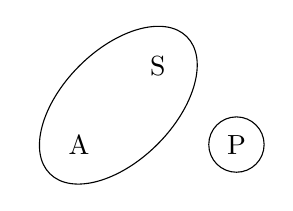
\begin{tikzpicture}
\node (S) at (1,1) {S};
\node (A) at (0,0) {A};
\node (P) at (2,0) {P};

\draw (0.5,0.5) ellipse [x radius=3.5em, y radius=2em, rotate=45];
\draw (P) circle [radius=1em];
\end{tikzpicture}

\a\label{ex:subject_ergabs}%
ergative--absolutive alignment (S/P---A):\medskip

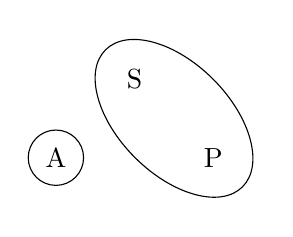
\begin{tikzpicture}
\node (S) at (1,1) {S};
\node (A) at (0,0) {A};
\node (P) at (2,0) {P};

\draw (1.5,0.5) ellipse [x radius=3.5em, y radius=2em, rotate=-45];
\draw (A) circle [radius=1em];
\end{tikzpicture}

\xe
\end{figure}

\citet{dixon2010a} defines a subject as \textcquote[76]{dixon2010a}{the entity
about which something is affirmed or denied}. He goes on to explain that,
ignoring copular clauses like \fw{We are tired and thirsty}, every language has
two varieties of clauses, intransitive\index{verbs!intransitive} ones, where the verb\index{verbs} has just one core
argument, and transitive\index{verbs!transitive} ones, where the verb\index{verbs} has two core arguments. A basic
definition based on this is given by the chart in (\ref{ex:subject}). It shows
the definition of the notion of subject for both nominative--accusative
languages and ergative--absolutive languages. Languages of the world differ
based on how they prefer to treat the two nominal relations of a transitive
verb\index{verbs!transitive} in relation to intransitive verbs\index{verbs!intransitive}: they may have a strong preference to
either treat the agent\index{semantic role!agent} (A)---the entity that prototypically acts in some
way---or the patient\index{semantic role!patient}/undergoer/theme\index{semantic role!theme} (P)---the entity which is prototypically
affected or handled by the action in some way---the same as S, the sole
argument of an intransitive verb\index{verbs!intransitive}. In the former case, the language is said to
have \Nom{}--\Acc{} alignment (\ref{ex:subject_nomacc}) with S/A being the
nominative subject, whereas in the latter case (\ref{ex:subject_ergabs}), the
language is said to have \Erg{}--\Abs{} alignment with S/P being the absolutive
subject. \citet{comrie1989} illustrates this difference with an example from
Chukchi, which we will here contrast with English\index{English}:\footnote{In English\index{English},
\fw{you} is the same for both singular and plural as well as subjective and
objective case, which is why I replaced it with the less ambiguous
\fw{her} in (\ref{ex:engchuk_eng}).}

\begin{figure}[h]
%\needspace{5\baselineskip}%
\pex\label{ex:engchuk_eng}
\a\label{ex:engchuk_eng1}\begingl
	\gla I came //
	\glb $\underbrace{\text{\Fsg{}.\Nom{}}}_{\text{S}}$
		come.\Pst{} //
\endgl

\a\label{ex:engchuk_eng2}\begingl
	\gla I saw her //
	\glb $\underbrace{\text{\Fsg{}.\Nom{}}}_{\text{S/A}}$
		see.\Pst{}
		$\underbrace{\text{\TsgF{}.\Obl{}}}_{\text{P}}$
		//
\endgl

\xe
\end{figure}

\begin{figure}[h]
%\needspace{5\baselineskip}%
\pex~\label{ex:engchuk_chuk}%
Chukchi \parencite[adapted from][104]{comrie1989}:
\a\label{ex:engchuk_chuk1}\begingl
	\gla ɣəm tə-yet-ɣʔek //
	\glb $\underbrace{\text{\Fsg{}.\Abs{}}}_{\text{S}}$
		came-\Fsg{} //
	\glft `I came.' //
\endgl

\a\label{ex:engchuk_chuk2}\begingl
	\gla ɣəm-nan ɣət tə-lʔu-ɣət //
	\glb $\underbrace{\text{\Fsg{}.\Erg{}}}_{\text{A}}$
		$\underbrace{\text{\Ssg{}.\Abs{}}}_{\text{S/P}}$
		saw-\Fsg{}-\Ssg{} //
	\glft `I saw thee.' //
\endgl

\xe
\end{figure}

While English\index{English} treats the actor of the intransitive sentence
(\ref{ex:engchuk_eng1}) the same as that of the transitive one
(\ref{ex:engchuk_eng2})---both sentences use \fw{I} in the nominative---Chukchi
appears to use a different pronoun for the actor of the intransitive sentence
(\ref{ex:engchuk_chuk1}) than for the actor of the transitive one
(\ref{ex:engchuk_chuk2})---absolutive \fw{ɣəm} versus ergative \fw{ɣəmnan},
respectively. At least in Standard English\index{English}, it would be ungrammatical to use
the pronoun \fw{me} in place of \fw{I} in (\ref{ex:engchuk_eng2}), since
\fw{me} can only be used for first-person objects of the verb, but not for
subjects of transitive clauses.

However, \citet{comrie1989} also urges to consider that grammatical relations
and their representation in morphology are not always as clear-cut as in the
example above. While he characterizes the prototypical subject as the
intersection of agent\index{semantic role!agent} and topic\index{grammatical function!topic} as far as cross-linguistic evidence is
concerned \citep[107]{comrie1989}, he also points out that subjects do not
necessarily have to unite all the properties typically associated with them
\citep[110]{comrie1989}. This seems to be the case, with Tagalog\index{Tagalog}, for instance,
as observed by both \citet{schachter1976} and \citet{kroeger1991}, and may
considerably complicate making a definitive statement.

Moreover, \citet{comrie1989} points out that statistically, languages of the
world show a strong preference for \Nom{}--\Acc{} alignment, possibly due to
the fact that human perception values actors as more relevant to discourse than
patients\index{semantic role!agent}, which is why actors are far more likely also to be pragmatic topics\index{grammatical function!topic}
\citep[120]{comrie1989}. Yet, though, dominantly \Nom{}--\Acc{}-aligned
languages may show a bias towards an \Erg{}--\Abs{} treatment, for instance, of
resultative constructions. On the other hand, dominantly \Erg{}--\Abs{}
languages show a bias towards a \Nom{}--\Acc{} treatment, for instance, of
addressees of imperatives \citep[116--119]{comrie1989}.

According to \citet{carnie2013}, from the point of view of constituent
structure (which is key in Generative Grammar), a subject is conventionally
understood as a \textcquote[221]{carnie2013}{DP that has the property
indicated by the predicate phrase. What the sentence is about. In most
sentences, this surfaces in the specifier of [the tense phrase]}. However, as
we have seen above, this notion is challenged by languages such as Tagalog\index{Tagalog}
\citep[225]{kroeger1991}. What \citet{carnie2013} refers to in terms of
constituent structure was basically already indicated by (\ref{ex:basicsvo}),
except with different labels; the example is repeated here for convenience as
(\ref{ex:basicsvo2}). For systemic reasons, \citet{carnie2013} refers to a DP\index{phrase types!determiner phrase}
subject which serves as the specifier of a TP. This corresponds to the subject
NP\index{phrase types!noun phrase} and the IP\index{phrase types!inflectional phrase} here. Unlike \textsc{gg}, \Lfg{}\index{Lexical-functional grammar} treats tense\index{tense} as a semantic
feature, not as a functional head with a fixed position in constituent
structure, hence the difference in labeling.

\begin{figure}
\ex\label{ex:basicsvo2}
\begin{forest}
[IP
	[NP
		[\textsc{subject}]
	]
	[\xbar{I}
		[\xhead{I}
			[\textsc{(auxiliary)}]
		]
		[VP
			[\xbar{V}
				[\xhead{V}
					[\textsc{verb}]
				]
				[NP
					[\textsc{object}]
				]
			]
		]
	]
]
\end{forest}
\xe
\end{figure}

\Lfg{}\index{Lexical-functional grammar} defines a subject function, \Subj{}. Which argument of the verb\index{verbs} the
subject is mapped onto is understood to be based on the relative prominence of
the subject argument along some dimension compared to other arguments. For
instance, \Nom{}--\Acc{} languages prefer the semantically most prominent
available role of a verb's\index{verbs} argument structure, \Erg{}--\Abs{} languages instead
pick the argument most affected by the actor's action, and active languages
focus on the argument in control of the action \citep[95--96]{bresnan2016}. The
mapping between grammatical functions like \Subj{} and the lexical components
that make it up also does not need to be a one-to-one correspondence, since
\Lfg{}\index{Lexical-functional grammar} allows for the distributed exponence of grammatical features like in the
example of Warlpiri\index{Warlpiri} in (\ref{ex:warlastruct}). The only condition is that
grammatical functions be uniquely defined within their minimal f-structure
\citep[45]{bresnan2016}. As (\ref{ex:warlastruct}) shows, multiple NPs in
different positions in the constituent structure may feed semantic information
to a single function defined by the argument structure of the verb\index{verbs}.

\begin{figure}
\ex\label{ex:warlastruct}
\begingl[glwordalign=center]
\glpreamble Warlpiri \citep[325]{bresnan2016}: //
\gla {~\hspace{1.5em}} {} chase {\quad\normalfont ⟨} agent {\quad} patient 
{\normalfont ⟩} {} //
\glb {} {[}
	\Pred{}\tikzmark{warlastruct_Pred}
	{}
	\Subj{}\tikzmark{warlastruct_Subj}
	{}
	\Obj{}\tikzmark{warlastruct_Obj}
	{}
	{]} //
\endgl

\begin{forest}
[IP
	[{NP~\tikzmark{warlastruct_ERGNP1}}
		[{...-\Erg{}}, roof]
	]
	[\xbar{I}
		[I, minimum width=5em]
		[S, minimum width=5em
			[{\tikzmark{warlastruct_V}~V}]
			[{NP~\tikzmark{warlastruct_ABSNP1}}
				[{...-\Abs{}}, roof]
			]
			[{NP~\tikzmark{warlastruct_ERGNP2}}
				[{...-\Erg{}}, roof]
			]
			[{NP~\tikzmark{warlastruct_ABSNP2}}
				[{...-\Abs{}}, roof]
			]
		]
	]
]
\end{forest}
\begin{tikzpicture}[remember picture, overlay]
\draw [-latex, min distance=1cm]
	([yshift=1ex]{pic cs:warlastruct_V})
	to [out=west, in=south]
	([xshift=-1em, yshift=-.5ex]{pic cs:warlastruct_Pred});

\draw [-latex, min distance=1cm]
	([yshift=1ex]{pic cs:warlastruct_ERGNP1})
	to [out=east, in=south]
	([xshift=-.75em, yshift=-.5ex]{pic cs:warlastruct_Subj});
\draw [-latex, min distance=1cm]
	([yshift=1ex]{pic cs:warlastruct_ERGNP2})
	to [out=east, in=south]
	([xshift=-.75em, yshift=-.5ex]{pic cs:warlastruct_Subj});

\draw [-latex, min distance=1cm]
	([yshift=1ex]{pic cs:warlastruct_ABSNP1})
	to [out=east, in=south]
	([xshift=-.5em, yshift=-.5ex]{pic cs:warlastruct_Obj});
\draw [-latex, min distance=1cm]
	([yshift=1ex]{pic cs:warlastruct_ABSNP2})
	to [out=east, in=south]
	([xshift=-.5em, yshift=-.5ex]{pic cs:warlastruct_Obj});
\end{tikzpicture}
\xe
\end{figure}

The subject role \thetaroof{} is defined as \textcquote[330]{bresnan2016} {the
most prominent semantic role of a predicator}, thus signifies the logical
subject. Furthermore, \citet{bresnan2016} devise two a-structure features,
[±\,o] (objective) and [±\,r] (restrictive). According to this classification,
\Subj{} is assigned the features [–\,r, –\,o], since the subject is not
restricted to a certain semantic role, nor needs to have a semantic
role.\footnote{This ought to make \citet{kroeger1991}'s analysis compatible to
\Lfg{}\index{Lexical-functional grammar} as well.} Also, subjects do not complement transitive predicators like
objects do, so they are not `objective'. \citet{bresnan2016}'s lexical mapping
theory assumes that all languages have subjects, which goes counter to
\textcites{schachter1976}{schachter2015}'s claim that subjects are possibly not
universal \citep[330--331]{bresnan2016}.

\index{grammatical function!subject|)}

\subsection{Topic}
\label{subsec:topic}
\index{grammatical function!topic|(}

The notion of topic refers essentially to who or what a longer stretch of
conversation is about. \citet{givon1983} defines the topic of a `thematic
paragraph'---as he calls a coherent unit of discourse above the level of a
single sentence---as \textcquote[8]{givon1983}{the continuity marker, the
\fw{leitmotif}}. The topic is thus

\blockcquote[8]{givon1983}{the participant \emph{most crucially involved} in
the action sequence running through the paragraph; it is the participant most
closely associated with the higher-level \enquote{theme} of the paragraph; and
finally, it is the participant most likely to be coded as the \emph{primary
topic}---or grammatical subject\index{grammatical function!subject}---of the vast majority of sequentially-ordered
clauses/sentences comprising the thematic paragraph.}

This indicates that topic and subject\index{grammatical function!subject} are closely related concepts, as already
mentioned above in reference to \citet{comrie1989}. Languages employ various
means to indicate topics; right- and left-dislocation, as known from English\index{English},
or topic-marking particles as in Japanese\index{Japanese} and Korean\index{Korean}, are only two among many
possibilities \citep[174]{dixon2010a}.

Topicality also interfaces with definiteness in that chain-initial topics may
be definite (already introduced into discourse) or indefinite (newly introduced
into discourse), while chain-medial topics and chain-final topics are always
expected to be definite \citep[10]{givon1983}. \citet[171]{dixon2010a} adds
that topic NPs\index{phrase types!noun phrase} are coreferential with arguments of clauses immediately
preceding or following the current clause. Moreover, the strategy of
passivization (in \Nom{}--\Acc{} languages) or of antipassivization (in 
\Erg{}--\Abs{} languages) exists, among others, in order to keep a certain
discourse item persistent in the highly topical subject position even if it
would otherwise be the object of the clause. This is related in turn to the
notion of syntactic pivot in clause coordination \citep[172]{dixon2010a}.

\index{grammatical function!topic|)}

\subsection{Focus}
\label{subsec:focus}
\index{grammatical function!focus|(}

Regarding the definition of focus, \citet[174]{dixon2010a} only mentions
contrastive focus, which basically raises the prominence of a certain NP\index{phrase types!noun phrase} within
a single clause. It is not necessary for the focused NP\index{phrase types!noun phrase} to be coordinated with
another NP\index{phrase types!noun phrase} by `or'. \citet{dixon2010a} also warns that focus is often confused
with topic\index{grammatical function!topic}. Perhaps this is in part also, as \citet{bresnan2016} mention, due
to the fact that English\index{English} may use the topic position for either topic or focus
under certain circumstances
\parencite[98]{bresnan2016}:

\ex\label{ex:engfoc}%
Q: What did you name your cat?\\
A: \textsc{rosie} I named her. (\fw{Rosie} = \Foc{})
\xe

The answer to a \fw{wh}-question\index{questions} is considered focused, so \fw{Rosie} in
(\ref{ex:engfoc}) is the focus in `I named her \textsc{rosie}'. However, in the
example above, \fw{Rosie} is fronted, which following \citet{givon1983},
constitutes a disruptive action used to establish a new topic of conversation:
left-dislocation in languages with rigid SVO word order such as English\index{English} is
typically associated with low topic continuity, and left-dislocated NPs\index{phrase types!noun phrase} can be
found most often as initiating a topic chain \citep[32]{givon1983}.

\index{grammatical function!focus|)}

\section{Tests on subjecthood}
\label{subsec:subjecthood}
\index{grammatical function!subject|(}

As initially mentioned, Ayeri was originally conceived under an impression of
what was described in the quote by \citet{cowan1995} above in terms of `trigger
language' (also compare \cite{schachter2015}). That is, in simple declarative
statements, the semantic macrorole of a definite NP is marked on the verb. This
is itself a very basic account of what can be observed in Tagalog\index{Tagalog} and other
Philippine languages, compare (\ref{ex:tagmarking}) (emphasis
mine).\footnote{The italicizing in (\ref{ex:tagmarking}) is not supposed to be
read as marking contrastive focus\index{grammatical function!focus}---this is one of the `mistakes' that led to
Ayeri's system, basically, besides then also mixing up focus\index{grammatical function!focus} and topic\index{grammatical function!topic}.}
Further effects will be discussed in more detail below.

\begin{figure}
%\needspace{3\baselineskip}
\pex\label{ex:tagmarking}%
Tagalog (\cite[14]{kroeger1991}, adapted from \cite[135]{foleyvanvalin1984}):
\a\label{ex:tagmarking_av}\begingl
	\gla B-\textbf{um}-ili \textbf{ang=lalake} ng=isda sa=tindahan. //
	\glb \Pfv{}.\Av{}-buy \Nom{}=man \Gen{}=fish \Dat{}=store //
	\glft `\emph{The man} bought fish at the store.' //
\endgl

\a\label{ex:tagmarking_ov}\begingl
	\gla B-in-ili-\textbf{Ø} ng=lalake \textbf{ang=isda} sa=tindahan. //
	\glb \Pfv{}-buy-\Ov{} \Gen{}=man \Nom{}=fish \Dat{}=store //
	\glft `The man bought \emph{the fish} at the store.' //
\endgl

\a\label{ex:tagmarking_dv}\begingl
	\gla B-in-ilh-\textbf{an} ng=lalake ng=isda \textbf{ang=tindahan.} //
	\glb \Pfv{}-buy-\Dv{} \Gen{}=man \Gen{}=fish \Nom{}=store //
	\glft `The man bought fish \emph{at the store}.' //
\endgl

\a\label{ex:tagmarking_iv}\begingl
	\gla \textbf{Ip}-in-\textbf{am}-bili ng=lalake ng=isda 
		\textbf{ang=pera.} //
	\glb \Iv{}-\Pfv{}-buy \Gen{}=man \Gen{}=fish \Nom{}=money //
	\glft `The man bought fish \emph{with the money}.' //
\endgl

% Tagalog example is missing in Kroeger (1991), present in Kroeger (1993: 14)
% (print edition of PhD thesis, Google Books BV9O0Kk5WcMC)
% \a\label{ex:tagmarking_bv}\begingl
% 	\gla I-b-in-ili ng=lalake ng=isda \textbf{ang=bata.} //
% 	\glb \Bv{}-\Pfv{}-buy \Gen{}=man \Gen{}=fish \Nom{}=child //
% 	\glft `The man bought fish \emph{for the child}.' //
% \endgl

\xe
\end{figure}

The examples in (\ref{ex:tagmarking}) show variations on the same sentence,
differing in the distribution of the definite NP which \citet{kroeger1991}
classifies as being the subject of the respective sentence on syntactic
grounds. The subject NPs are marked with the clitic \fw{ang}, and their role in
the clause is reflected by the voice marking on the verb (the root is \fw{bili}
`buy'): in (\ref{ex:tagmarking_av}) the subject is the actor, in
(\ref{ex:tagmarking_ov}) it is the object, in (\ref{ex:tagmarking_dv}) it is a
location, and in (\ref{ex:tagmarking_iv}) it is an instrument. What is
remarkable is that this voice marking goes beyond mere
passivization,\footnote{Note that \citet{kroeger1991} avoids the terms
\emph{active voice} and \emph{passive voice} that \citet{schachter2015} objects
to as inappropriate, even though what Tagalog\index{Tagalog} does essentially appears to work
along those lines, except in a more generalized way.} so even the oblique
arguments of (\ref{ex:tagmarking}cd) can become subjects of their respective
clauses. Ayeri is at least superficially similar, compare
(\ref{ex:ayrmarking}).

\begin{figure}
\pex\label{ex:ayrmarking}
\a\label{ex:ayrmarking_at}\begingl
	\gla \textbf{ang}=int-ya \textbf{ayon-Ø} inun-ley moton-ya //
	\glb \AgtT{}=buy-\TsgM{} man-\Top{} fish-\PargI{} store-\Loc{} //
	\glft `\emph{The man}, he bought fish at the store.' //
\endgl

\a\label{ex:ayrmarking_pt}\begingl
	\gla \textbf{le}=int-ya ayon-ang \textbf{inun-Ø} moton-ya //
	\glb \PatTI{}=buy-\TsgM{} man-\Aarg{} fish-\Top{} store-\Loc{} //
	\glft `\emph{The fish}, the man bought it at the store.' //
\endgl

\a\label{ex:ayrmarking_loct}\begingl
	\gla \textbf{ya}=int-ya ayon-ang inun-ley \textbf{moton-Ø} //
	\glb \LocT{}=buy-\TsgM{} man-\Aarg{} fish-\PargI{} store-\Top{} //
	\glft `\emph{The store}, the man bought fish there.' //
\endgl

\a\label{ex:ayrmarking_inst}\begingl
	\gla \textbf{ri}=int-ya ayon-ang inun-ley \textbf{pangis-Ø} //
	\glb \InsT{}=buy-\TsgM{} man-\Aarg{} fish-\PargI{} money-\Top{} //
	\glft `\emph{The money}, the man bought fish with it.' //
\endgl

% \a\label{ex:ayrmarking_datt}\begingl
% 	\gla yam=int-ya ayon-ang inun-ley \textbf{gan-Ø} //
% 	\glb \DatT{}=buy-\TsgM{} man-\Aarg{} fish-\PargI{} child-\Top{} //
% 	\glft `\emph{The child}, the man bought fish for it.' //
% \endgl

\xe
\end{figure}

Like Tagalog\index{Tagalog}, Ayeri marks a privileged NP\index{phrase types!noun phrase} on the verb\index{verbs}, however, in Ayeri, this
is the topic\index{grammatical function!topic}, not the subject (this will be subject to further scrutiny below).
Unlike in Tagalog\index{Tagalog}, the marked NP\index{phrase types!noun phrase} is not marked by a particle, but by the very
absence of case marking on the NP\index{phrase types!noun phrase} itself. The marker corresponding to the role
of the topic\index{grammatical function!topic} NP\index{phrase types!noun phrase} appears as a clitic in the shape of the corresponding NP's\index{phrase types!noun phrase} case
marker in its proclitic form at the left-most edge of the clause, before the
verb\index{verbs} (compare sections \ref{subsec:case} and \ref{sec:verbs}). While the marker
on the verb\index{verbs} is thus related to nominal case markers in Ayeri, Tagalog\index{Tagalog} uses a
number of affixes for voice marking which are not obviously related to case
markers on nouns. For instance, non-subject actors are marked by the genitive
clitic \fw{ng} (pronounced \fw{nang}), while actor voice is marked by \fw{mag-}
or \fw{-um-} \parencites[74, 78]{schachterotanes1972}[16--18]{kroeger1991}. In
Ayeri, on the other hand, non-topic\index{grammatical function!topic} animate agents\index{case!agent} are marked on NPs\index{phrase types!noun phrase} by
\rayr{/ANF}{-ang} or \rayr{ANF}{ang}, and animate agent-topics\index{grammatical function!topic} are marked on
the verb\index{verbs} by \rayr{ANF}{ang} as well.

\subsection{Verb agreement}
\label{subsec:verbagr}
\index{agreement|(}
\index{verbs|(}

One of the most prominent features of Ayeri with regards to verbs and their
relation to subjects\index{grammatical function!subject} is verb agreement with third-person\index{person} NPs\index{phrase types!noun phrase}. This was already
discussed at length in \autoref{clitics_postverb_person} 
(p.~\pageref{clitics_postverb_person}\,ff.) and \autoref{sec:verbs}. Hence, I
will only give basic information here.

\citet{kroeger1991} mentions that Tagalog\index{Tagalog} has optional plural agreement of
predicates with the nominative NP if the nominative argument of the clause is
plural. This is independent of whether the nominative argument is also the
actor of the clause or not \citep[24--25]{kroeger1991}, compare
(\ref{ex:tagagr}). The arrows in (\ref{ex:tagagr}) mark government and
agreement relationships: the verb governs role and case assignment (top arrow),
while the nominative NP controls plural agreement on the verb (bottom arrow).
As the arrows illustrate, the relationship between the assignment of the
subject role and thus nominative case and plural agreement on the verb are
symmetric: the verb agrees in both (\ref{ex:tagagr_1}) and (\ref{ex:tagagr_2})
with the respective nominative NP, whether it is the agent\index{semantic role!agent} or not.

\begin{figure}
\pex\label{ex:tagagr}%
Tagalog (adapted from \cite[24--25]{kroeger1991}, from 
	\cite[122--123]{aspillera1969}):
\a\label{ex:tagagr_1}\begingl[aboveglbskip=1.5em, aboveglftskip=1.75em]
	\gla nagsisi-kain na ang=mga=bata ng=hapunan //
	\glb \Av{}.\Impf{}.\Pl{}-eat\tikzmark{tagagra_targ} already 
		$\underbrace{\text{\Nom{}=\Pl{}=child}\tikzmark{tagagra_ctrl1}}_%
			{\text{S/A}\tikzmark{tagagra_ctrl2}}$
		$\underbrace{\text{\Gen{}=\smash{supper}}}_%
			{\text{P}}$ //
	\glft `The children are eating their supper already.' //
\endgl
\begin{tikzpicture}[remember picture, overlay]
\draw [-latex]
	([xshift=-.5*width{"av.impf.pl-eat"}, yshift=2.25ex]{pic cs:tagagra_targ})
	|- ++ (north:.75em) -|
	([xshift=-.5*width{"nom=pl=child"}, yshift=2.25ex]{pic cs:tagagra_ctrl1});

\draw [-latex]
	([xshift=-.5*width{"s/a"},yshift=-.75ex]{pic cs:tagagra_ctrl2}) 
	|- ++ (south:.75em) -|
	([xshift=-.5*width{"av.impf.pl-eat"}, yshift=-.75ex]{pic cs:tagagra_targ});
\end{tikzpicture}

\a\label{ex:tagagr_2}\begingl[aboveglbskip=1.5em, aboveglftskip=1.75em]
	\gla pagsu-sulat-in ni=Linda ang=mga=liham //
	\glb \Fut{}.\Pl{}-write-\Ov{}\tikzmark{tagagrb_targ}
		$\underbrace{\text{\Gen{}=Linda}}_%
			{\text{A}}$
		$\underbrace{\text{\Nom{}=\Pl{}=letter}\tikzmark{tagagrb_ctrl1}}_%
			{\text{S/P}\tikzmark{tagagrb_ctrl2}}$ //
	\glft `Linda will write the letters.' //
\endgl
\begin{tikzpicture}[remember picture, overlay]
\draw [-latex]
	([xshift=-.5*width{"fut.pl-write-ov"}, yshift=2.25ex]{pic cs:tagagrb_targ})
	|- ++ (north:.75em) -|
	([xshift=-.5*width{"nom=pl=letter"}, yshift=2.25ex]{pic cs:tagagrb_ctrl1});

\draw [-latex]
	([xshift=-.5*width{"s/p"},yshift=-.75ex]{pic cs:tagagrb_ctrl2}) 
	|- ++ (south:.75em) -|
	([xshift=-.5*width{"fut.pl-write-ov"}, yshift=-.75ex]%
		{pic cs:tagagrb_targ});
\end{tikzpicture}
\xe
\end{figure}

Person\index{person} agreement in Ayeri is fixed to the agent\index{semantic role!agent} NP\index{phrase types!noun phrase} in canonical cases, whether
it is the topic\index{grammatical function!topic} of the clause or not. In (\ref{ex:ayragr_1}), we can see the
verb determine that the agent\index{semantic role!agent} argument is also the topic\index{grammatical function!topic}, with the verb
agreeing itself in person\index{person} with the agent\index{semantic role!agent}: \rayr{AgYaanF}{Ajān} is a male name;
the verb corresponds with masculine agreement. In (\ref{ex:ayragr_2}), however,
the relation is asymmetric in that the marking on the verb shows that the
patient\index{semantic role!patient} argument is the topic\index{grammatical function!topic}, while the verb still displays masculine person\index{person}
agreement. We know that the verb agrees with \rayr{AgYaanF}{Ajān} rather than
with \rayr{pil}{Pila} because the latter is a female name, so the verb should
have feminine agreement if it were to agree with the patient\index{semantic role!patient} NP\index{phrase types!noun phrase}. The verb
instead continues to agree with the agent\index{semantic role!agent} NP\index{phrase types!noun phrase} in spite of not being the topic\index{grammatical function!topic} of
the clause. Topicalization\index{grammatical function!topic} appears to have no influence on the distribution of
person\index{person} agreement on the verb; the agent\index{semantic role!agent} NP\index{phrase types!noun phrase} remains the subject\index{grammatical function!subject}. This is a very
\Nom{}--\Acc{} trait.

\begin{figure}
\pex\label{ex:ayragr}
\a\label{ex:ayragr_1}\begingl[aboveglcskip=1.5em, aboveglftskip=1.75em]
	\gla {Ang manya} Ajān {sa Pila}. //
	\glb ang=man-ya {Ø=Ajān} {sa=Pila} //
	\glc \AgtT{}=greet-\TsgM{}\tikzmark{ayragra_targ}
		$\underbrace{\text{\Top{}=\smash{Ajān}}\tikzmark{ayragra_ctrl1}}_%
		{\text{S/A}\tikzmark{ayragra_ctrl2}}$
		$\underbrace{\text{\Parg{}=Pila}}_{\text{P}}$ //
	\glft `Ajān, he greets Pila.' //
\endgl
\begin{tikzpicture}[remember picture, overlay]
\draw [-latex]
	([xshift=-.5*width{"at=greet-3sg.m"}, yshift=2.25ex]{pic cs:ayragra_targ})
	|- ++ (north:.75em) -|
	([xshift=-.5*width{"top=Ajān"}, yshift=2.25ex]{pic cs:ayragra_ctrl1});

\draw [-latex]
	([xshift=-.5*width{"s/a"},yshift=-.75ex]{pic cs:ayragra_ctrl2}) 
	|- ++ (south:.75em) -|
	([xshift=-.5*width{"at=greet-3sg.m"}, yshift=-.75ex]{pic cs:ayragra_targ});
\end{tikzpicture}

\a\label{ex:ayragr_2}\begingl[aboveglcskip=1.5em, aboveglftskip=1.75em]
	\gla {Sa manya} {ang Ajān} Pila. //
	\glb sa=man-ya {ang=Ajān} {Ø=Pila} //
	\glc \PatT{}=greet-\TsgM{}\tikzmark{ayragrb_targ}
		$\underbrace{\text{\Aarg{}=\smash{Ajān}}}_%
			{\text{S/A}\tikzmark{ayragrb_ctrl2}}$
		$\underbrace{\text{\Top{}=Pila}\tikzmark{ayragrb_ctrl1}}_{\text{P}}$ //
	\glft `Pila, Ajān greets her.' //
\endgl
\begin{tikzpicture}[remember picture, overlay]
\draw [-latex]
	([xshift=-.5*width{"pt=greet-3sg.m"}, yshift=2.25ex]{pic cs:ayragrb_targ})
	|- ++ (north:.75em) -|
	([xshift=-.5*width{"top=Pila"}, yshift=2.25ex]{pic cs:ayragrb_ctrl1});

\draw [-latex]
	([xshift=-.5*width{"s/a"},yshift=-.75ex]{pic cs:ayragrb_ctrl2}) 
	|- ++ (south:.75em) -|
	([xshift=-.5*width{"pt=greet-3sg.m"}, yshift=-.75ex]{pic cs:ayragrb_targ});
\end{tikzpicture}

\xe
\end{figure}

In agentless\index{semantic role!agent} clauses, however, the verb agrees with the patient\index{semantic role!patient} argument, which
makes Ayeri less typical a \Nom{}--\Acc{} language, and more similar in this
regard to what an \Erg{}--\Abs{} language would be expected to do.
Passivization of a transitive clause as a strategy for keeping the topic\index{grammatical function!topic}
constant as a subject\index{grammatical function!subject} is essentially preempted by Ayeri's use of a topic\index{grammatical function!topic}
particle in the verb phrase\index{phrase types!verb phrase}. Hence, a sentence like (\ref{ex:ayragr2_1})---as a
parallel to (\ref{ex:tagagr_2})---sounds odd, while (\ref{ex:ayragr2_2}) is
fine.

\begin{figure}
\pex\label{ex:ayragr2}
\a\label{ex:ayragr2_1}\ljudge\ques%
\begingl[aboveglcskip=1.5em, aboveglftskip=1.75em]
	\gla {Sa manye} {ang Ajān} Pila. //
	\glb sa=man-ye {ang=Ajān} {Ø=Pila} //
	\glc \PatT{}=greet-\TsgF{}\tikzmark{ayragr2a_targ}
		$\underbrace{\text{\Aarg{}=\smash{Ajān}}}_{\text{A}}$
		$\underbrace{\text{\Top{}=Pila}\tikzmark{ayragr2a_ctrl1}}_%
			{\text{S/P}\tikzmark{ayragr2a_ctrl2}}$ //
	\glft `Pila, she is greeted by Ajān.' //
\endgl
\begin{tikzpicture}[remember picture, overlay]
\draw [-latex]
	([xshift=-.5*width{"pt=greet-3sg.f"}, yshift=2.25ex]{pic cs:ayragr2a_targ})
	|- ++ (north:.75em) -|
	([xshift=-.5*width{"top=Pila"}, yshift=2.25ex]{pic cs:ayragr2a_ctrl1});

\draw [-latex]
	([xshift=-.5*width{"s/p"},yshift=-.75ex]{pic cs:ayragr2a_ctrl2}) 
	|- ++ (south:.75em) -|
	([xshift=-.5*width{"pt=greet-3sg.f"}, yshift=-.75ex]%
		{pic cs:ayragr2a_targ});
\end{tikzpicture}

\a\label{ex:ayragr2_2}\begingl[aboveglftskip=1.75em]
	\gla Manye {sa Pila}. //
	\glb man-ye Ø=Pila //
	\glc greet-\TsgF{}\tikzmark{ayragr2b_targ}
		$\underbrace{\text{\Parg{}=Pila}}_%
			{\text{S/P}\tikzmark{ayragr2b_ctrl}}$ //
	\glft `Pila is greeted.' //
\endgl
\begin{tikzpicture}[remember picture, overlay]
\draw [-latex]
	([xshift=-.5*width{"s/p"},yshift=-.75ex]{pic cs:ayragr2b_ctrl}) 
	|- ++ (south:.75em) -|
	([xshift=-.5*width{"pt=greet-3sg.f"}, yshift=-.75ex]%
		{pic cs:ayragr2b_targ});
\end{tikzpicture}

\xe
\end{figure}

\index{verbs|)}
\index{agreement|)}

\subsection{Syntactic pivot}
\label{subsubsec:pivot}
\index{coordination|(}

Since we have just dealt with aspects of syntactic alignment and found that
Ayeri behaves a little oddly with regards to this, it may be interesting to
perform another test on declarative statements and their syntactic pivot as
well. A simple test which \citet[111--114]{comrie1989} describes in this regard
is to test coreference in coordinated\index{coordination} clauses. In coordinated\index{coordination} clauses, it seems
to be not uncommon for the subject of the second conjunct to drop out. Thus, in
English\index{English}, which behaves very much in terms of \Nom{}--\Acc{} alignment in this
regard, we get the result in (\ref{ex:engpivot}).

\begin{figure}
\pex[belowexskip=1.75em]\label{ex:engpivot}%
%	English:
	\a\label{ex:engpivot_1}%
		$\underbrace{The\ cat}_{\text{A}}$ 
		$hunts$ $\underbrace{the\ mouse}_{\text{P}}$.
	
	\a\label{ex:engpivot_2}%
		$\underbrace{The\ cat}_{\text{S}}$ $comes\ here.$
	
	\a\label{ex:engpivot_3}%
		$\underbrace{The\ mouse}_{\text{S}}$ $comes\ here.$
	
	\a\label{ex:engpivot_4}%
		$\underbrace{The\ cat}_{\text{A}\tikzmark{engpivot_ant}}$
		$hunts$
		$\underbrace{the\ mouse}_{\text{P}}$
		$and$
		$\underbrace{ }_{\text{S}\tikzmark{engpivot_drop}}$
		$comes\ here.$

\begin{tikzpicture}[remember picture, overlay]
\draw [-latex] ([xshift=-.25em,yshift=-.75ex]{pic cs:engpivot_ant}) 
|- ++ (south:.75em) -| ([xshift=-.25ex, yshift=-.75ex]{pic cs:engpivot_drop});
\end{tikzpicture}
\xe
\end{figure}

In the English\index{English} example in (\ref{ex:engpivot}), \fw{the cat} constitutes the
coreferential subject in (\ref{ex:engpivot_4}). This NP is the intransitive
subject S of (\ref{ex:engpivot_2}) and the agent A of (\ref{ex:engpivot_1}).
English\index{English} thus has \Nom{}--\Acc{} alignment, since it typically treats S and A
alike. In an \Erg{}--\Abs{} language, then, we would expect the opposite case:
S and P should be treated alike.

\begin{figure}
\pex\label{ex:dyirpivot}%
Dyirbal \parencite[adapted from][112]{comrie1989}:
\a\label{ex:dyirpivot_1}
	\begingl
		\gla {balan dʸugumbil} {baŋgul yaṛaŋgu} balgan //
		\glb $\underbrace{\text{\Det{} woman-\Abs{}}}_{\text{P}}$
			$\underbrace{\text{\Det{} man-\Erg{}}}_{\text{A}}$ hit //
		\glft `The man hit the woman.' //
	\endgl
	
\a\label{ex:dyirpivot_2}%
	\begingl
		\gla {bayi yaṛa} baninʸu //
		\glb $\underbrace{\text{\Det{} man-\Abs{}}}_{\text{S}}$ came.here //
		\glft `The man came here.' //
	\endgl
	
\a\label{ex:dyirpivot_3}%
	\begingl
		\gla {balan dʸugumbil} baninʸu //
		\glb $\underbrace{\text{\Det{} woman-\Abs{}}}_{\text{S}}$ 
			came.here //
		\glft `The woman came here.' //
	\endgl
	
\a\label{ex:dyirpivot_4}%
	\begingl[aboveglftskip=1.75em]
		\gla {balan dʸugumbil} {baŋgul yaṛaŋgu} balgan, {} baninʸu //
		\glb $\underbrace{\text{\Det{} woman-\Abs{}}}_%
				{\text{P}\tikzmark{dyirpivot_ant}}$
			$\underbrace{\text{\Det{} man-\Erg{}}}_{\text{A}}$
			hit 
			$\underbrace{ }_{\text{S}\tikzmark{dyirpivot_drop}}$
			came.here //
		\glft `The man hit the woman, and [the woman] came here.' //
	\endgl

\begin{tikzpicture}[remember picture, overlay]
\draw [-latex] ([xshift=-.25em,yshift=-.75ex]{pic cs:dyirpivot_ant}) 
|- ++ (south:.75em) -| ([xshift=-.25ex, yshift=-.75ex]{pic cs:dyirpivot_drop});
\end{tikzpicture}
\xe
\end{figure}

This is indeed the case in the examples of Dyirbal\index{Dyirbal} in (\ref{ex:dyirpivot}),
where we find that \fw{balan dʸugumbil} `the woman' is coreferential in
(\ref{ex:dyirpivot_4}). This is the S of (\ref{ex:dyirpivot_3}), and the P of
(\ref{ex:dyirpivot_1}). Dyirbal\index{Dyirbal}, thus, treats S and P alike, as predicted for
an \Erg{}--\Abs{} language---at least in this case, since
\citet[113]{comrie1989} also explains that \Fsg{} and \Ssg{} pronouns in
Dyirbal\index{Dyirbal} behave in terms of \Nom{}--\Acc{}. \citet{comrie1989} also notes that
some languages do not show a clear preference for whether the A or P of the
transitive clause in the first conjunct is the preferred reference of the S of
the intransitive clause in the second conjunct.

For Tagalog\index{Tagalog}, as \citet{kroeger1991} explains, \textcquote[30]{kroeger1991}{the
deletion is not obligatory but null nominative arguments are always interpreted
as referring to the nominative argument of the main clause}. Due to the way
Tagalog\index{Tagalog} treats subjects, however, the nominative argument can be formed by
either NP in (\ref{ex:tagpivot}) with the voice marked accordingly on the
verb.\footnote{Thus, compare the English\index{English} passive sentence \fw{Marvin$_i$ was
asked by Derek$_j$ before he$_i$ left} with (\ref{ex:tagpivot_1}). In English\index{English},
the reference of \fw{he} is ambiguous between the syntactic subject \fw{Marvin}
and the agent \fw{Derek}, however. As we have seen above, though, Tagalog\index{Tagalog} would
also be able to make a subject of an oblique argument, not just of the
patient\index{semantic role!patient}/theme\index{semantic role!theme} or the recipient\index{semantic role!recipient}. The actor of the Tagalog\index{Tagalog} sentence is also
basically an object, not demoted to an adverbial as in English\index{English}
\citep[38--44]{kroeger1991}.}

\begin{figure}
\pex\label{ex:tagpivot}%
Tagalog (\cite[adapted from][31]{kroeger1991}, from 
	\cite[151--152]{ramoscena1990}):
\a\label{ex:tagpivot_1}%
\begingl[aboveglbskip=1.5em, aboveglftskip=1.75em]
	\gla tinanong ni=Derek si=Marvin, bago umalis {} //
	\glb \Pfv{}-ask-\Ov{}\tikzmark{tagpivot1_vc}
		$\underbrace{\text{\Gen{}=Derek}}_{\text{A}}$
		$\underbrace{\text{\Nom{}=Marvin}\tikzmark{tagpivot1_anta}}_%
			{\text{P}\tikzmark{tagpivot1_antb}}$
		before \Pfv{}.\Av{}-leave\tikzmark{tagpivot1_vc2}
		$\underbrace{ \tikzmark{tagpivot1_anta2}}_%
			{\text{S}\tikzmark{tagpivot1_drop}}$
		//
	\glft `Derek asked Marvin before [Marvin] left.' //
\endgl
\begin{tikzpicture}[remember picture, overlay]
\draw [-latex] 
	([xshift=-.5*width{"pfv-ask-ov"},yshift=+2.25ex]{pic cs:tagpivot1_vc})
	|- ++ (north:.75em) -|
	([xshift=-.5*width{"nom=Marvin"}, yshift=2.25ex]{pic cs:tagpivot1_anta});

\draw [-latex]
	([xshift=-.125em,yshift=-.75ex]{pic cs:tagpivot1_antb}) 
	|- ++ (south:.75em) -|
	([xshift=-.25ex, yshift=-.75ex]{pic cs:tagpivot1_drop});

\draw [-latex] 
	([xshift=-.5*width{"pfv.av-leave"},yshift=+2.25ex]{pic cs:tagpivot1_vc2})
	|- ++ (north:.75em) -|
	([xshift=0ex, yshift=2.25ex]{pic cs:tagpivot1_anta2});
\end{tikzpicture}

\a\label{ex:tagpivot_2}%
\begingl[aboveglbskip=1.5em, aboveglftskip=1.75em]
	\gla nagtanong si=Derek kay=Marvin, bago umalis {} //
	\glb \Pfv{}.\Av{}-ask\tikzmark{tagpivot2_vc}
		$\underbrace{\text{\Nom{}=Derek}\tikzmark{tagpivot2_anta}}_%
			{\text{A}\tikzmark{tagpivot2_antb}}$
		$\underbrace{\text{\Dat{}=Marvin}}_{\text{P}}$
		before \Pfv{}.\Av{}-leave\tikzmark{tagpivot2_vc2}
		$\underbrace{ \tikzmark{tagpivot2_anta2}}_%
			{\text{S}\tikzmark{tagpivot2_drop}}$
		//
	\glft `Derek asked Marvin before [Derek] left.' //
\endgl
\begin{tikzpicture}[remember picture, overlay]
\draw [-latex] 
	([xshift=-.5*width{"pfv.av-ask"},yshift=+2.25ex]{pic cs:tagpivot2_vc})
	|- ++ (north:.75em) -|
	([xshift=-.5*width{"nom=Derek"}, yshift=2.25ex]{pic cs:tagpivot2_anta});

\draw [-latex]
	([xshift=-.125em,yshift=-.75ex]{pic cs:tagpivot2_antb}) 
	|- ++ (south:.75em) -|
	([xshift=-.25ex, yshift=-.75ex]{pic cs:tagpivot2_drop});

\draw [-latex] 
	([xshift=-.5*width{"pfv.av-leave"},yshift=+2.25ex]{pic cs:tagpivot2_vc2})
	|- ++ (north:.75em) -|
	([xshift=0ex, yshift=2.25ex]{pic cs:tagpivot2_anta2});
\end{tikzpicture}

\xe
\end{figure}

What can be observed in Tagalog\index{Tagalog} is that in (\ref{ex:tagpivot_1}), the dropped S
argument in the second conjunct, \fw{bago umalis ...} `before ...\ leaves', is
coreferential with \fw{Marvin}, since he is marked as the subject of the first
conjunct. Since \fw{Marvin} is the theme (P) of \fw{tanong} `ask', the clause
needs to be marked for objective voice. On the other hand, in
(\ref{ex:tagpivot_2}), it is \fw{Derek} who is the subject of the clause, so it
is also he who leaves; the verb in the first conjunct clause is marked for
active voice according to the asker as the actor (A) being the subject.

In order to now investigate what the situation is in Ayeri, let us return to
our initial set of examples. These examples featured two animals which in Ayeri
are treated both as animate neuters. Anaphoric reference is thus potentially
ambiguous between \xayr{prlF}{paral}{cat} and \xayr{pFrbr}{prabara}{mouse} in
(\ref{ex:ayrpivot}).

\begin{figure}
\pex\label{ex:ayrpivot}%
\a\label{ex:ayrpivot_1}
	\begingl
		\gla Ang @ kimbyo paral prabarās. //
		\glb ang= kimb-yo paral-Ø prabara-as //
		\glc \AgtT{}= hunt-\TsgN{}
			$\underbrace{\text{cat-\Top{}}}_{\text{A}}$
			$\underbrace{\text{mouse-\Parg{}}}_{\text{P}}$ //
		\glft `The cat hunts the mouse.' //
	\endgl
	
\a\label{ex:ayrpivot_2}%
	\begingl
		\gla Sahayo paralang edaya. //
		\glb saha-yo paral-ang edaya //
		\glc come-\TsgN{} $\underbrace{\text{cat-\Aarg{}}}_{\text{S}}$
			here //
		\glft `The cat comes here.' //
	\endgl
	
\a\label{ex:ayrpivot_3}%
	\begingl
		\gla Sahayo prabarāng edaya. //
		\glb saha-yo prabara-ang edaya //
		\glc come-\TsgN{} $\underbrace{\text{mouse-\Aarg{}}}_{\text{S}}$
			here //
		\glft `The mouse comes here.' //
	\endgl
	
\a\label{ex:ayrpivot_4}%
	\begingl[aboveglftskip=1em]
		\gla Ang @ kimbyo paral prabarās nay sahayong edaya. //
		\glb ang= kimb-yo paral-Ø prabara-as nay saha=yong edaya  //
		\glc \AgtT{}= hunt-\TsgN{}
			$\underbrace{\text{cat-\Top{}}}_{\text{A}\tikzmark{ayrpivot_ctrl}}$
			$\underbrace{\text{mouse-\Parg{}}}_{\text{P}}$
			and
			come=$\underbrace{\text{\smash{\TsgN{}}.\Aarg{}}}_%
				{\text{S}\tikzmark{ayrpivot_targ}}$
			here //
		\glft `The cat, it hunts the mouse, and it comes here.' //
	\endgl

\begin{tikzpicture}[remember picture, overlay]
\draw [-latex]
	([xshift=-.25em,yshift=-.75ex]{pic cs:ayrpivot_ctrl}) 
	|- ++ (south:.75em) -|
	([xshift=-.25em,yshift=-.75ex]{pic cs:ayrpivot_targ});
\end{tikzpicture}
\xe
\end{figure}

While it is possible in Ayeri to not repeat the coreferential NP\index{phrase types!noun phrase} in a conjunct
clause verbatim, Ayeri still appears to avoid an empty subject\index{grammatical function!subject} slot. Thus, the
verb\index{verbs} \xayr{shyoNF}{sahayong}{it comes} in (\ref{ex:ayrpivot_4}) displays a
pronominal clitic\index{clitics}, \xayr{/yoNF}{-yong}{it}, which constitutes the resumptive
subject\index{grammatical function!subject} pronoun\index{pronouns} of the clause. In (\ref{ex:ayrpivot_4}) at least, this pronoun\index{pronouns}
is coreferential with the subject\index{grammatical function!subject} in the first conjunct,
\xayr{prlF}{paral}{cat}. Seeing as Tagalog\index{Tagalog} switches the subject\index{grammatical function!subject} around by
altering the voice marking on the verb\index{verbs}, it is certainly illustrative to check
how Ayeri fares if the topic\index{grammatical function!topic} is swapped to \xayr{pFrbr}{prabara}{mouse}.

\begin{figure}[h]
\ex\label{ex:ayrpivot2}
\begingl[aboveglftskip=1em]
	\gla Sa @ kimbyo paralang prabara nay sahayong edaya. //
	\glb sa= kimb-yo paral-ang prabara-Ø nay saha=yong edaya  //
	\glc \PatT{}= hunt-\TsgN{}
		$\underbrace{\text{cat-\Aarg}}_{\text{A}}$
		$\underbrace{\text{mouse-\Top{}}}_{\text{P}\tikzmark{ayrpivot2_ctrl}}$
		and
		come=$\underbrace{\text{\smash{\TsgN{}}.\Aarg{}}}_%
			{\text{S}\tikzmark{ayrpivot2_targ}}$
		here //
	\glft `The mouse, the cat hunts it, and it comes here.' //
\endgl

\begin{tikzpicture}[remember picture, overlay]
\draw [-latex]
	([xshift=-.25em,yshift=-.75ex]{pic cs:ayrpivot2_ctrl}) 
	|- ++ (south:.75em) -|
	([xshift=-.25em,yshift=-.75ex]{pic cs:ayrpivot2_targ});
\end{tikzpicture}
\xe
\end{figure}

In (\ref{ex:ayrpivot2}), the resumptive pronoun\index{pronouns!resumptive} is indicated to not refer to
the first conjunct's agent\index{semantic role!agent}/subject\index{grammatical function!subject}, \rayr{prlF}{paral}, but to its
theme\index{semantic role!theme}/object, \rayr{pFrbr}{prabara}. This may be explained by topicalization:\index{grammatical function!topic}
the sentence is about the mouse, so the underspecified argument in the second
conjunct, in absence of topic\index{grammatical function!topic} marking that would indicate otherwise,
corresponds to the topic\index{grammatical function!topic}. Interestingly, the result is structurally similar to
the example of Tagalog\index{Tagalog} in (\ref{ex:tagpivot}) above. It is too early yet,
however, to conclude that what was called `topic'\index{grammatical function!topic} so far is the subject\index{grammatical function!subject} after
all; Ayeri is merely not completely unambiguous\index{ambiguity} in this context. Since Tagalog\index{Tagalog}
allows any NP of a clause to be the subject, as illustrated by
(\ref{ex:tagmarking}), let us test whether the behavior just described for
Ayeri also holds in other contexts of topicalization.\index{grammatical function!topic} Example 
(\ref{ex:ayrpivot3}) presents sentences of differently case-marked topic\index{grammatical function!topic} NPs\index{phrase types!noun phrase}
each, but in every case, the agent\index{semantic role!agent} NP\index{phrase types!noun phrase} and the topicalized\index{grammatical function!topic}NP\index{phrase types!noun phrase} consist of a human
referent. Both referents share the same person\index{person} features so that the verb\index{verbs} in the
coordinated\index{coordination} intransitive clause\index{verbs!intransitive} can theoretically license either of them as its
subject\index{grammatical function!subject}.

\begin{figure}
\pex\label{ex:ayrpivot3}
\a\label{ex:ayrpivot3_dat}\begingl
	\gla Yam @ ilya ang @ Akan ilonley {} @ Maran nay sarayāng. //
	\glb yam= il-ya ang= Akan ilon-ley Ø= Maran nay sara=yāng //
	\glc \DatT{}= give-\TsgM{} \Aarg{}= Akan present-\PargI{} \Top{}= Maran
		and leave=\TsgM{}.\Aarg{} //
	\glft `Maran, Akan gives him a present, and he leaves.' (Maran leaves) //
\endgl

\a\label{ex:ayrpivot3_gen}\begingl
	\gla Na @ pahya ang @ Maran ilonley {} @ Diyan nay sarayāng. //
	\glb na= pah-ya ang= Maran ilon-ley Ø= Diyan nay sara=yāng //
	\glc \GenT{}= take.away-\TsgM{} \Aarg{}= Maran present-\PargI{} \Top{}=
		Diyan and leave=\TsgM{}.\Aarg{} //
	\glft `Diyan, Maran takes the present away from him, and he leaves.' (Diyan
		leaves) //
\endgl

\a\label{ex:ayrpivot3_loc}\begingl
	\gla Ya @ bahaya ang @ Diyan {} @ Maran nay sarayāng. //
	\glb ya= baha-ya ang= Diyan Ø= Maran nay sara=yāng //
	\glc \LocT{}= baha-\TsgM{} \Aarg{}= Diyan \Top{}= Maran and 
		leave=\TsgM{}.\Aarg{} //
	\glft `Maran, Diyan shouts at him, and he leaves.' (Maran leaves) //
\endgl

\a\label{ex:ayrpivot3_ins}\begingl
	\gla Ri @ su-sunca ang @ Diyan ilonley {} @ Sedan nay sarayāng. //
	\glb ri= su\til{}sunt-ya ang= Diyan ilon-ley Ø= Sedan nay sara=yāng. //
	\glc \InsT{}= \Iter{}\til{}claim-\TsgM{} \Aarg{}= Diyan present-\PargI{}
		\Top{}= Sedan and leave=\TsgM{}.\Aarg{} //
	\glft `Sedan, Diyan reclaims the present with his help, and he leaves.'
		(Sedan leaves) //
\endgl

\a\label{ex:ayrpivot3_cau}\begingl
	\gla Sā @ pinyaya ang @ Maran tatamanyam {} @ Sedan nay sarayāng. //
	\glb sā= pinya-ya ang= Maran tataman-yam Ø= Sedan nay sara=yāng //
	\glc \CauT{}= ask-\TsgM{} \Aarg{}= Maran forgiveness-\Dat{} \Top{}= Sedan
		and leave=\TsgM{}.\Aarg{} //
	\glft `Sedan, he makes Maran ask for forgiveness, and he leaves.' (Sedan
		leaves) //
\endgl

\xe
\end{figure}

In each of the sentences in (\ref{ex:ayrpivot3}), it is the topicalized\index{grammatical function!topic} NP\index{phrase types!noun phrase}
which is identified as the antecedent for \xayr{sryaaNF}{sarayāng}{he leaves}.
Does this mean Ayeri does, in fact, use Austronesian alignment? While the
examples in (\ref{ex:ayrpivot3}) certainly suggest it, let us not forget that
the verb\index{verbs} in the coordinated\index{coordination} clause could theoretically pick either the agent\index{semantic role!agent} NP\index{phrase types!noun phrase}
or the topicalized\index{grammatical function!topic} NP\index{phrase types!noun phrase} of the first conjunct as its subject\index{grammatical function!subject}. Things look
slightly different, however, if the reference of the verb\index{verbs} is unambiguous\index{ambiguity}, for
instance, because the topicalized\index{grammatical function!topic} argument cannot logically be the agent\index{semantic role!agent} of the
coordinated\index{coordination} clause, as shown in (\ref{ex:ayrpivot4}).

\begin{figure}[h]
\ex\label{ex:ayrpivot4}\begingl[aboveglcskip=1.5em, aboveglftskip=2.5em]
	\gla {Le ilya} {ang Akan} ilon {yam Maran} nay sarayāng. //
	\glb {le=il-ya} {ang=Akan} ilon-Ø {\Dat{}=Maran} nay sara=yāng //
	\glc \PatTI{}=give-\TsgM{}\tikzmark{ayrpivot4_top}
		$\underbrace{\text{\Aarg{}=Akan}}_{\text{A}\tikzmark{ayrpivot4_ctrl}}$
		$\underbrace{\text{\smash{present}-\Top{}}\tikzmark{ayrpivot4_top2}}_%
			{\text{P}\tikzmark{ayrpivot4_ctrl2}}$
		$\underbrace{\text{\Dat{}=Maran}}_{\text{R}}$
		and
		leave=$\underbrace{\text{\smash{\TsgM{}}.\Aarg{}}}_%
			{\text{S}\tikzmark{ayrpivot4_targ}}$
		//
	\glft `The present, Akan gives it to Maran, and he leaves.' 
		(Akan leaves) //
\endgl
\begin{tikzpicture}[remember picture, overlay]
\draw [-latex] 
	([xshift=-.5*width{"pt.inan=give-3sg.m"},yshift=+2.25ex]
		{pic cs:ayrpivot4_top})
	|- ++ (north:.75em) -|
	([xshift=-.5*width{"present-top"},yshift=2.25ex]{pic cs:ayrpivot4_top2});

\draw [-latex]
	([xshift=-.125em,yshift=-.75ex]{pic cs:ayrpivot4_ctrl}) 
	|- ++ (south:.75em) -|
	([xshift=-.25ex, yshift=-.75ex]{pic cs:ayrpivot4_targ});

\draw [-latex, dashed]
	([xshift=-.125em,yshift=-.75ex]{pic cs:ayrpivot4_ctrl2}) 
	|- ++ (south:1.5em) -|
	([xshift=-.25ex, yshift=-.75ex]{pic cs:ayrpivot4_targ});

\node (a) at ([yshift={-.75ex - 1.5em}]{pic cs:ayrpivot4_ctrl2}) {};
\node (b) at ([yshift={-.75ex - 1.5em}]{pic cs:ayrpivot4_targ}) {};
\node (x) at ($(a)!0.5!(b)$) {\bfseries\larger ×};
\end{tikzpicture}
\xe
\end{figure}

In (\ref{ex:ayrpivot4}), the first conjunct's verb\index{verbs}, as the head of its clause,
specifies that the topic\index{grammatical function!topic} of the clause is the patient\index{semantic role!patient} (P), which is embodied by
\xayr{IlonF}{ilon}{present}. This NP\index{phrase types!noun phrase}, however, is not a very typical agent\index{semantic role!agent} for
the verb\index{verbs} in the second conjunct, \xayr{sr/}{sara-}{leave}. Besides, this verb\index{verbs}
is conjugated so as to require an animate masculine controller, whereas
\rayr{IlonF}{ilon} is inanimate, as shown by the topic\index{grammatical function!topic} marker \rayr{le}{le}.
\rayr{IlonF}{ilon} is thus not a suitable controller for \rayr{sryaaNF}
{sarayāng}, since their person-feature\index{person} values clash with each other---the 
\Anim{} and \Gend{}\index{gender} values in particular, see (\ref{ex:animgendclash}).

\begin{figure}
\begin{morphlex}
\pex\label{ex:animgendclash}
\a \adjustbox{valign=t}{%
\begin{tabu} {\usetabu{morphlex}}
\rayr{\larger IlonF}{ilon}
	& N
	& \begin{tabular}[t]{l l l}
		\ups{\Pred} & = & `present' \\
		\ups{\Index} & = & ↓ \\
		\quad\downs{\Pers} & = & \Third \\
		\quad\downs{\Num} & = & \Sg{} \\
		\textbf{\quad\downs{\Anim}} & \textbf{=} & \textbf{$-$} \\
		\textbf{\quad\downs{\Gend}} & \textbf{=} & \textbf{\Inan} \\
	\end{tabular}
\end{tabu}%
}

\a\adjustbox{valign=t}{%
\begin{tabu} {\usetabu{morphlex}}
\rayr{\larger sryaaNF}{sarayāng}
	& I
	& \begin{tabular}[t]{l l l}
		\ups{\Pred} & = & \astruct{leave}{\ups{\Subj}} \\
		\ups{\Subj} & = & ↓ \\
		\quad\downs{\Pred} & = & `$pro$' \\
		\quad\downs{\Pers} & = & \Third \\
		\quad\downs{\Num} & = & \Sg \\
		\textbf{\quad\downs{\Anim}} & \textbf{=} & \textbf{$+$} \\
		\textbf{\quad\downs{\Gend}} & \textbf{=} & \textbf{\M} \\
		\quad\downs{\Case} & = & \Aarg \\
	\end{tabular}
\end{tabu}%
}
\xe
\end{morphlex}
\end{figure}

As before, there are two masculine NPs\index{phrase types!noun phrase} in the first conjunct which form
suitable antecedents on behalf of being animate masculine as required: the
agent\index{semantic role!agent} (A) \rayr{AknF}{Akan} and the recipient\index{semantic role!recipient} (R) \rayr{mrnF}{Maran}. Of the
remaining non-topic\index{grammatical function!topic} NPs\index{phrase types!noun phrase}, Ayeri considers the agent\index{semantic role!agent} to rank higher as a
secondary topic\index{grammatical function!topic} on the thematic hierarchy\index{hierarchy} than the recipient\index{semantic role!recipient}, compare 
(\ref{ex:themhier}). The agent\index{semantic role!agent} hence forms the preferred controller for
\rayr{sryaaNF}{sarayāng}. In cases where the topic\index{grammatical function!topic} in the first conjunct can
safely be ruled out as the controller of the pronominal in the second conjunct,
the syntactic pivot, thus, defaults\index{default} to the highest-ranking semantically
coherent NP\index{phrase types!noun phrase}. In most cases, Ayeri will therefore group the intransitive\index{verbs!intransitive} subject\index{grammatical function!subject}
and the transitive agent\index{semantic role!agent} together.

\begin{figure}[h]
\ex\label{ex:themhier}%
	Thematic hierarchy\index{hierarchy} \citep[329]{bresnan2016}:\medskip \\
	agent > beneficiary > experiencer/goal > instrument > patient/theme >
	locative
\xe
\end{figure}

For most verbs\index{verbs}, this is also reflected by case marking, as we have
seen above in (\ref{ex:ayrpivot}): the S of an intransitive clause\index{verbs!intransitive} receives the
same case marker as the A of a transitive clause:
\rayr{/ANF}{-ang}/\rayr{ANF}{ang} for animate\index{animacy} referents, and
\rayr{/reNF}{reng}/\rayr{ENF}{eng} for inanimate\index{animacy} referents (compare
\autoref{subsubsec:agent}). The case described initially, where the topic\index{grammatical function!topic}
marking basically determines the controller of the coordinated\index{coordination} intransitive
clause\index{verbs!intransitive}, which is reminiscent of Tagalog's\index{Tagalog} syntax, is essentially a strategy to
disambiguate\index{ambiguity} between two possible controllers for the same target. When only
one of the referents in the transitive conjunct is eligible as the controller
of the subject\index{grammatical function!subject} of the intransitive\index{verbs!intransitive} conjunct at the same time, A and P are
regularly indicated by person\index{person} agreement\index{agreement}, since Ayeri requires a resumptive
pronominal clitic\index{clitics} in the intransitive clause\index{verbs!intransitive}, as indicated above. The affix on
the verb\index{verbs} thus has the status of a pronominal predicator, compare
(\ref{ex:ayrpivot5}).

\begin{figure}
\pex\label{ex:ayrpivot5}
\a\label{ex:ayrpivot5_1}\begingl[aboveglftskip=2.5em]
	\gla Ang @ tinisaya Lita {sa Kumang} nay sarayāng. //
	\glb ang= tinisa-ya Ø=Lita sa=Kumang nay sara=yāng //
	\glc \AgtT{}= hug-\TsgM{}
		$\underbrace{\text{\Top{}=Lita}}_{\text{A}\tikzmark{ayrpivot5a_ctrl1}}$
		$\underbrace{\text{\Parg{}=\smash{Kumang}}}_%
			{\text{P}\tikzmark{ayrpivot5a_ctrl2}}$
		and 
		leave=$\underbrace{\text{\smash{\TsgM{}}.\Aarg{}}}_%
			{\text{S}\tikzmark{ayrpivot5a_targ}}$ //
	\glft `Lita, he hugs Kumang, and he leaves.' //
\endgl
\begin{tikzpicture}[remember picture, overlay]
\draw [-latex]
	([xshift=-.125em,yshift=-.75ex]{pic cs:ayrpivot5a_ctrl1}) 
	|- ++ (south:.75em) -|
	([xshift=-.25ex, yshift=-.75ex]{pic cs:ayrpivot5a_targ});

\draw [-latex, dashed]
	([xshift=-.125em,yshift=-.75ex]{pic cs:ayrpivot5a_ctrl2}) 
	|- ++ (south:1.5em) -|
	([xshift=-.25ex, yshift=-.75ex]{pic cs:ayrpivot5a_targ});

\node (a) at ([yshift={-.75ex - 1.5em}]{pic cs:ayrpivot5a_ctrl2}) {};
\node (b) at ([yshift={-.75ex - 1.5em}]{pic cs:ayrpivot5a_targ}) {};
\node (x) at ($(a)!0.5!(b)$) {\bfseries\larger ×};
\end{tikzpicture}

\a\label{ex:ayrpivot5_2}\begingl[aboveglftskip=2.5em]
	\gla Ang @ tinisaya Lita {sa Kumang} nay sarayeng. //
	\glb ang= tinisa-ya Ø=Lita sa=Kumang nay sara=yeng //
	\glc \AgtT{}= hug-\TsgM{}
		$\underbrace{\text{\Top{}=Lita}}_{\text{A}\tikzmark{ayrpivot5b_ctrl1}}$
		$\underbrace{\text{\Parg{}=\smash{Kumang}}}_%
			{\text{P}\tikzmark{ayrpivot5b_ctrl2}}$
		and 
		leave=$\underbrace{\text{\smash{\TsgF{}}.\Aarg{}}}_%
			{\text{S}\tikzmark{ayrpivot5b_targ}}$ //
	\glft `Lita, he hugs Kumang, and she leaves.' //
\endgl

\begin{tikzpicture}[remember picture, overlay]
\draw [-latex]
	([xshift=-.125em,yshift=-.75ex]{pic cs:ayrpivot5b_ctrl2}) 
	|- ++ (south:1.5em) -|
	([xshift=-.25ex, yshift=-.75ex]{pic cs:ayrpivot5b_targ});

\draw [-latex, dashed]
	([xshift=-.125em,yshift=-.75ex]{pic cs:ayrpivot5b_ctrl1}) 
	|- ++ (south:.75em) -|
	([xshift=-.25ex, yshift=-.75ex]{pic cs:ayrpivot5b_targ});

\node (a) at ([yshift={-.75ex - .75em}]{pic cs:ayrpivot5b_ctrl1}) {};
\node (b) at ([yshift={-.75ex - .75em}]{pic cs:ayrpivot5b_targ}) {};
\node (x) at ($(a)!0.5!(b)$) {\bfseries\larger ×};
\end{tikzpicture}
\xe
\end{figure}

In (\ref{ex:ayrpivot5_1}), the verb\index{verbs} in the second conjunct, \xayr{sryaaNF}
{sarayāng}{he leaves} is marked for a masculine third-person\index{person} subject\index{grammatical function!subject}. The only
available controller in the first con\-junct is \rayr{lit}{Lita} on behalf of
being male, since \rayr{kumNF}{Kumang} is female. Hence, in
(\ref{ex:ayrpivot5_2}) the verb\index{verbs} of the intransitive\index{verbs!intransitive} conjunct, \xayr{sryeNF}
{sarayeng}{she leaves}, finds its controller only in \rayr{kumNF}{Kumang}.

\index{coordination|)}

\subsection{Quantifier float}
\label{subsec:quantfloat}
\index{quantifiers|(}

Another property usually associated with subjects\index{grammatical function!subject} is the ability of quantifiers
referring to the subject\index{grammatical function!subject} NP\index{phrase types!noun phrase} to `float' into the VP\index{phrase types!verb phrase}. This is possible also in
English\index{English}, consider, for instance, (\ref{ex:engqfloat}).

\begin{figure}[h]
\pex\label{ex:engqfloat}%
English:
\a\label{ex:engqfloat_1}%
	\fw{\textbf{All} the children are writing letters.}
\a\label{ex:engqfloat_2}%
	\fw{The children are \textbf{all} writing letters.}
\xe
\end{figure}

Both of these sentences are equal in meaning: for all children in the set,
every child is writing an unspecified amount of letters. It is not the case in
(\ref{ex:engqfloat_2}) that for an unspecified amount of children, together
they write the total amount of letters. \fw{All} refers to \fw{the children} in
both cases, even though \fw{all} is not placed in the subject\index{grammatical function!subject} NP, \fw{the
children}, in (\ref{ex:engqfloat_2}). \citet{kroeger1991} mentions an example
from \citet{schachterotanes1972} concerning \fw{lahat} `all', which is also
able to float into a position right after the sentence-initial verb from the NP
it normally modifies and which it would normally occur in, as
(\ref{ex:tagqfloat}) shows.

\begin{figure}
\pex\label{ex:tagqfloat}%
Tagalog (adapted from \cite[22]{kroeger1991}, from 
	\cite[501]{schachterotanes1972}):
\a\label{ex:tagqfloat_1}\begingl
	\gla sumusulat lahat ang=mga=bata ng=mga=liham //
	\glb \Av{}.\Impf{}-write all \Nom{}=\Pl{}=child \Gen{}=\Pl{}=letter //
	\glft `All the children are writing letters.'\\
		\textit{Not:} *`The children are writing all the letters.' //
\endgl

\a\label{ex:tagqfloat_2}\begingl
	\gla sinusulat lahat ng=mga=bata ang=mga=liham //
	\glb \Impf{}-write-\Ov{} all \Gen{}=\Pl{}=child \Nom{}=\Pl{}=letter //
	\glft `The/some children write all the letters.'\\
		\textit{Not:} *`All the children are writing letters.' //
\endgl

\xe
\end{figure}

In (\ref{ex:tagqfloat_1}), \fw{lahat} `all' refers to the children, which
constitute the subject NP according to voice and case marking, while we get the
opposite case in (\ref{ex:tagqfloat_2}), where it refers to the letters, which
are marked as the subject this time. Of course, it is equally possible in
English\index{English} to say \fw{The letters are all written by the children}, where \fw{the
letters} is the subject that the floated \fw{all} refers to.

As pointed out in \autoref{sec:quantifiers}, a lot of clitic\index{clitics} quantifiers in
Ayeri have a double meaning as intensifiers\index{intensifiers}. For instance, \rayr{/IknF}{-ikan}
can refer to both quantities and qualities, meaning `much, many' or `very'
depending on context. Thus, many of the suffixed\index{suffixes} quantifiers, if appended to
the VP\index{phrase types!verb phrase}, are understood to modify the verb\index{verbs} as an intensifier\index{intensifiers} and are thus
unsuitable for floating. The only exception is \xayr{/ArilF}{-aril}{some},
which only pertains to NPs\index{phrase types!noun phrase} as a quantifier. However, since the floating of
suffixed\index{suffixes} quantifiers would produce readings which are ambiguous at best,
floating of \rayr{/ArilF}{-aril} is avoided as well. Example
(\ref{ex:ayrqfloat1}) shows an attempt to float \xayr{/henF}{\mbox{-hen}}{all}
into the IP\index{phrase types!inflectional phrase}, resulting in a meaning different from the sentence with the
unfloated particle for the reasons just stated above.

\begin{figure}[t]
\pex\label{ex:ayrqfloat1}
\a\label{ex:ayrqfloat1_1}\begingl
	\gla Ang @ tahanyan ganye-hen tamanyeley. //
	\glb ang= tahan-yan gan-ye-Ø=hen taman-ye-ley //
	\glc \AgtT{}= write-\TplM{} child-\Pl{}-\Top{}=all letter-\Pl{}-\PargI{} //
	\glft `The children, all of them are writing letters.' //
\endgl

\a\label{ex:ayrqfloat1_2}\ljudge\excl\begingl
	\gla Ang @ tahanyan-hen ganye tamanyeley. //
	\glb ang= tahan-yan=hen gan-ye-Ø taman-ye-ley //
	\glc \AgtT{}= write-\TplM{}=completely child-\Pl{}-\Top{}
		letter-\Pl{}-\PargI{} //
	\glft `\ques{}The children, they are completely writing letters.'\\
		\textit{Intended:} `The children, they are all writing letters.' //
\endgl

\xe
\end{figure}

Besides suffixed\index{suffixes} quantifiers, Ayeri also possesses free
quantifiers such as \xayr{sno}{sano}{both} or \xayr{diriNF}{diring}{several},
however. These free morphemes only have a quantifying reading, not an
intensifying one. They are thus suitable for floating, since they do not produce
ambiguities with regards to what is being modified, unlike their enclitic
counterparts.

\begin{figure}[t]
\pex\label{ex:ayrqfloat2}
\a\label{ex:ayrqfloat2_1}\begingl
	\gla Ang @ apayan yan sano layjya. //
	\glb ang= apa-yan yan-Ø sano lay-ye-ya //
	\glc \AgtT{}= laugh-\TplM{} boy-\Top{} both girl-\Pl{}-\Loc{} //
	\glft `The boys, both of them are laughing at the girls.' //
\endgl

\a\label{ex:ayrqfloat2_2}\begingl
	\gla Ang @ apayan sano yan layjya. //
	\glb ang= apa-yan sano yan-Ø lay-ye-ya //
	\glc \AgtT{}= laugh-\TplM{} both boy-\Top{} girl-\Pl{}-\Loc{} //
	\glft `The boys, they are both laughing at the girls.' //
\endgl
\xe
\end{figure}

Since, as described above, topicalization\index{grammatical function!topic} has no impact on what constitutes the
subject\index{grammatical function!subject}, meaning does not significantly change when the topic\index{grammatical function!topic} of a sentence
like (\ref{ex:ayrqfloat2_2}) is switched to the patient\index{semantic role!patient} in example 
(\ref{ex:ayrqfloat3_1}). Unlike in Tagalog\index{Tagalog} in (\ref{ex:tagqfloat_2}) above,
\xayr{ynNF}{yanang}{boy(s)} as the agent\index{semantic role!agent} NP\index{phrase types!noun phrase} remains the subject\index{grammatical function!subject}, and the
floated \rayr{sno}{sano} still refers to this NP\index{phrase types!noun phrase} rather than the locative NP\index{phrase types!noun phrase},
\xayr{ljye}{layye}{(at) the girls}. This fact is also reflected in the lack of
plural\index{number!plural} marking on \rayr{ynNF}{yanang}, since \rayr{sno}{sano} indicates the
NP's\index{phrase types!noun phrase} plurality\index{number!plural}. We would expect the forms \rayr{ynFye\_aNF}{yanjang} and
\rayr{lj}{lay} if \rayr{sno}{sano} were to refer to `the girls' rather than
`the boys', as in (\ref{ex:ayrqfloat3_2}).

\begin{figure}[t]
\pex\label{ex:ayrqfloat3}
\a\label{ex:ayrqfloat3_1}\begingl
	\gla Ya @ apayan sano yanang layye. //
	\glb ya= apa-yan sano yan-ang lay-ye-Ø //
	\glc \LocT{}= laugh-\TplM{} both boy-\Aarg{} girl-\Pl{}-\Top{} //
	\glft `The girls, the boys are both laughing at them.' //
\endgl

\a\label{ex:ayrqfloat3_2}\begingl
	\gla Ya @ apayan yanjang lay sano. //
	\glb ya= apa-yan yan-ye-ang lay-Ø sano //
	\glc \LocT{}= laugh-\TplM{} boy-\Pl{}-\Aarg{} girl-\Top{} both //
	\glft `The girls, the boys are laughing at both of them.' //
\endgl
\xe
\end{figure}

As we have seen above, the modification of subject\index{grammatical function!subject} pronouns\index{pronouns} with clitic\index{clitics}
quantifiers is avoided due to many of them serving a double role as
intensifiers\index{intensifiers} with related meanings which could be readily understood as
referring to the verb\index{verbs} instead of the pronoun\index{pronouns}. With free quantifiers, such as
\xayr{sno}{sano}{both} in (\ref{ex:freequantplcmt}), this problem does not
arise, however, so that there is no problem in placing them right after the
finite verb\index{verbs!finite}. Ambiguity may be in the phrase structure of the clause here, but
not at a functional level, as it is clear that the quantifier modifies the
subject\index{grammatical function!subject} pronoun\index{pronouns} due to semantic coherence.

\begin{figure}[t]
\ex\label{ex:freequantplcmt}
\begingl
	\gla Ang @ girenjan sano bahalanya. //
	\glb ang= girend=yan.Ø sano bahalan-ya //
	\glc \AgtT{}= arrive=\TplM{}.\Aarg{} both finish-\Loc{} //
	\glft `They arrived both at the finish.' //
\endgl\xe
\end{figure}

As mentioned in \autoref{subsec:reflrec}, it is possible for pronouns\index{pronouns} to be
modified by enclitic\index{clitics} intensifiers\index{intensifiers} indirectly by using
\xayr{sitNF}{sitang}{self} as an indeclinable dummy pronoun\index{pronouns} to carry the clitic\index{clitics}
so as to avoid ambiguity created by floating the clitic\index{clitics} right after the finite
verb\index{verbs!finite}. This is also possible for the purpose of quantification of pronouns\index{pronouns} with
clitic\index{clitics} quantifiers.

\begin{figure}[h]
\pex\label{ex:pronquant}
\a\label{ex:pronquant_1}\begingl
	\gla Ang @ girenjan panca sitang-hen bahalanya. //
	\glb ang= girend=yan.Ø panca sitang=hen bahalan-ya //
	\glc \AgtT{}= arrive=\TplM{}.\Aarg{} finally self=all finish-\Loc{} //
	\glft `All of them finally arrived at the finish.' //
\endgl

\a\label{ex:pronquant_2}\begingl
	\gla Ya @ girendtang panca sitang-hen bahalan. //
	\glb ya= girend=tang panca sitang=hen bahalan-Ø //
	\glc \LocT{}= arrive=\TplM{}.\Aarg{} finally self=all finish-\Top{} //
	\glft `The finish, all of them finally arrived there.' //
\endgl
\xe
\end{figure}

Since \rayr{sitNF}{sitang} is indeclinable, it is the pronominal clitic\index{clitics} which
carries inflection for case, as (\ref{ex:pronquant_2}) shows. An analysis of
\rayr{sitNF/henF}{sitang-hen} as `self.\Top{}=all' is therefore not possible.
Moreover, \rayr{/tNF sitNF/henF}{-tang sitang-hen} does not constitute a clitic\index{clitics}
cluster, because it is possible to place word material between the verb\index{verbs} and
\rayr{sitNF/henF}{sitang-hen}, as (\ref{ex:pronquant}) shows. See
\autoref{subsec:expsitang} for an analysis of dummy \rayr{sitNF}{sitang} in
terms of constituent and functional structure.

\index{quantifiers|)}

\subsection{Relativization}
\label{subsec:relz}
\index{relative clause|(}

\citet{kroeger1991} observes that in Tagalog\index{Tagalog}, only nominative arguments may be
relativized. He refers to \citet{keenancomrie1977}'s accessibility hierarchy\index{hierarchy} of
NPs\index{phrase types!noun phrase}, according to which, he reports, \textcquote[24]{kroeger1991}{if only a
single argument of any clause can be relativized, that argument must be the
subject}. That is, the argument in the main clause which is modified by a
relative clause must be the nominative argument, and there must not appear an
overt nominative argument in the relative clause itself. The verb in the
relative clause carries inflection for the role of the relativized argument in
the relative clause. Thus, (\ref{ex:tagrel_1}) is grammatical, while 
(\ref{ex:tagrel_2}) is not.

\begin{figure}[h]
\pex\label{ex:tagrel}%
Tagalog (\cite[24]{kroeger1991}, from \cite[141--142]{foleyvanvalin1984}):
\a\label{ex:tagrel_1}\begingl
	\gla bata=ng b-in-igy-an ng=lalake ng=isda //
	\glb child=\Lnk{} \Pfv{}-give-\Dv{} \Gen{}=man \Gen{}=fish //
	\glft `the child which was given fish by the man' //
\endgl

\a\label{ex:tagrel_2}\ljudge*\begingl
	\gla isda=ng nag-bigay ang=lalake sa=bata //
	\glb fish=\Lnk{} \Av{}-\Pfv{}-give \Nom{}=man \Dat{}=child //
\endgl
\xe
\end{figure}

Ayeri, however, has no such restrictions. Non-topic\index{grammatical function!topic} NPs\index{phrase types!noun phrase} may be relativized, and
relative clauses not uncommonly contain their own agent\index{semantic role!agent} NP\index{phrase types!noun phrase}. The relativized NP\index{phrase types!noun phrase}
may even be referred to in the relative clause by a resumptive pronoun\index{pronouns!resumptive} or
pronominal clitic\index{clitics}, since verbs\index{verbs} must not go uninflected. Since all NPs\index{phrase types!noun phrase} are
accessible for relativization, it is not a suitable criterion for testing
subjecthood.

\begin{figure}[h]
\ex\label{ex:ayrrel}\begingl
	\gla Ang @ ilya inunley ganyam inunaya si gumasayāng edaya. //
	\glb ang= il-ya inun-ley gan-yam inunaya-Ø si gum-asa=yāng edaya //
	\glc \AgtT{}= give-\TsgM{} fish-\PargI{} child-\Dat{} fisherman-\Top{} 
		\Rel{} work-\Hab{}=\TsgM{}.\Aarg{} here //
	\glft `The fisherman who used to work here, he gave fish to the child.' //
\endgl\xe
\end{figure}

In (\ref{ex:ayrrel}), \xayr{Inuny}{inunaya}{the fisherman}, is both the topic\index{grammatical function!topic}
of the clause and modified by a relative clause. He is referenced anaphorically
by the \TsgM{}.\Aarg{} suffix\index{suffixes} \rayr{/yaaNF}{\mbox{-yāng}} on the verb\index{verbs} in the
relative clause, since he is the actor in both. However, as the examples in 
(\ref{ex:ayrrel2}) show, these circumstances are not requirements for grammatical statements.

\begin{figure}[h]
\pex\label{ex:ayrrel2}
\a\label{ex:ayrrel2_1}\begingl
	\gla Ang @ ilya inunaya inunley ganyam si ang @ pyabasaye benanya-hen. //
	\glb ang= il-ya inunaya-Ø inun-ley gan-yam si ang= pyab-asa=ye.Ø 
		benan-ya=hen //
	\glc \AgtT{}= give-\TsgM{} fisherman-\Top{} fish-\PargI{} child-\Dat{}
		\Rel{} \AgtT{}= pass.by-\Hab{}=\TsgF{}.\Top{} morning-\Loc{}=every //
	\glft `The fisherman, he gave fish to the child which passes by every
		morning.' //
\endgl

\a\label{ex:ayrrel2_2}\begingl
	\gla Ang @ ilya inunaya ganyam inunley si petigayāng hiro. //
	\glb ang= il-ya inunaya-Ø gan-yam inun-ley si petiga=yāng hiro //
	\glc \AgtT{}= give-\TsgM{} fisherman-\Top{} child-\Dat{} fish-\PargI{}
		\Rel{} catch=\TsgM{}.\Aarg{} freshly //
	\glft `The fisherman, he gave fish which he caught freshly to the 
		child.' //
\endgl
\xe
\end{figure}

In (\ref{ex:ayrrel2_1}), the recipient\index{semantic role!recipient} NP\index{phrase types!noun phrase} \xayr{gnFymF}{ganyam}{to the child}
is not the topic\index{grammatical function!topic} of the clause, but it is modified by a relative clause anyway.
The relativized NP\index{phrase types!noun phrase} is again represented within the relative clause by means of
verb\index{verbs} morphology. The topic\index{grammatical function!topic} marker on the verb\index{verbs} identifies the person\index{person} suffix\index{suffixes} on
the verb\index{verbs} as the clause's topic\index{grammatical function!topic}. In (\ref{ex:ayrrel2_2}), it is likewise not the
topic\index{grammatical function!topic} NP\index{phrase types!noun phrase} which is relativized, but the patient\index{semantic role!patient} NP\index{phrase types!noun phrase} \xayr{InunFlej}{inunley}
{fish}. This NP\index{phrase types!noun phrase}, however, is not represented in the relative clause because the
verb\index{verbs} does not inflect for the role of the patient\index{semantic role!patient}, which the relativized NP\index{phrase types!noun phrase}
carries in the relative clause as well. There is no morphology to alter the
voice of the verb\index{verbs} in such a way that the matrix clause's patient\index{semantic role!patient} NP\index{phrase types!noun phrase} becomes the
subject\index{grammatical function!subject} of the relative clause. As (\ref{ex:ayrrel3}) illustrates, relative
clauses in Ayeri may even just consist of a predicative adjective\index{adjectives!predicative}. In these
cases, there is no case-marked noun\index{nouns} or topic\index{grammatical function!topic} contained in the relative clause.

\begin{figure}[h]
\ex\label{ex:ayrrel3}\begingl
	\gla Ang @ ilya inunaya ganyam inunley si hiro nay lepan. //
	\glb ang= il-ya inunaya-Ø gan-yam inun-ley si hiro nay lepan //
	\glc \AgtT{}= give-\TsgM{} fisherman-\Top{} child-\Dat{} fish-\PargI{}
	\Rel{} fresh and tasty //
	\glft `The fisherman, he gave fish which is fresh and tasty to the
		child.' //
\endgl\xe
\end{figure}

\index{relative clause|)}

\subsection{Control of secondary predicates}
\label{subsec:secpredctrl}

Secondary predicates in Tagalog\index{Tagalog} are interesting insofar as depictive adjectives
which occur after the verb always modify the nominative argument according to
\citet{kroeger1991}; compare the example in (\ref{ex:tagsecpred}).

\begin{figure}[h]
%\needspace{5\baselineskip}
\pex\label{ex:tagsecpred}
Tagalog \parencite[adapted from][29--30]{kroeger1991}:
\a\label{ex:tagsecpred_1}%
	\begingl[aboveglbskip=1.5em, aboveglftskip=1.75em]
	\gla naghain na lasing si=Maria ng=isda //
	\glb \Av.\Pfv-serve\tikzmark{tagsecpred1a_vbtop}%
		\tikzmark{tagsecpred1a_vbbot}
		\Lnk{}
		drunk\tikzmark{tagsecpred1a_adj}
		\Nom{}=Maria\tikzmark{tagsecpred1a_sbtop}\tikzmark{tagsecpred1a_sbbot}
		\Gen{}=fish\tikzmark{tagsecpred1a_obbot}
		//
	\glft `Maria served the fish drunk.' (Maria was drunk) //
\endgl
\begin{tikzpicture}[remember picture, overlay]
\draw [-latex]
	([xshift=-.5*width{"av.pfv-serve"}, yshift=2.25ex]%
		{pic cs:tagsecpred1a_vbtop})
	|- ++ (north:.75em) -|
	([xshift=-.5*width{"nom=Maria"}, yshift=2.25ex]%
		{pic cs:tagsecpred1a_sbtop});

\draw [-latex]
	([xshift=-.5*width{"drunk"}, yshift=-.75ex]{pic cs:tagsecpred1a_adj})
	|- ++ (south:.75em) -|
	([xshift=-.5*width{"nom=Maria"},yshift=-.75ex]{pic cs:tagsecpred1a_sbbot});
\end{tikzpicture}

\a\label{ex:tagsecpred_2}%
	\begingl[aboveglbskip=1.5em, aboveglftskip=1.75em]
	\gla inihain na hilaw ni=Maria ang=isda //
	\glb \Iv{}.\Pfv-serve\tikzmark{tagsecpred1b_vbtop}%
			\tikzmark{tagsecpred1b_vbbot}
		\Lnk{}
		raw\tikzmark{tagsecpred1b_adj}
		\Gen{}=Maria\tikzmark{tagsecpred1b_obbot}
		\Nom{}=fish\tikzmark{tagsecpred1b_sbtop}\tikzmark{tagsecpred1b_sbbot}
		//
	\glft `Maria served the fish raw.' (The fish was raw) //
\endgl
\begin{tikzpicture}[remember picture, overlay]
\draw [-latex]
	([xshift=-.5*width{"iv.pfv-serve"}, yshift=2.25ex]%
		{pic cs:tagsecpred1b_vbtop})
	|- ++ (north:.75em) -|
	([xshift=-.5*width{"nom=fish"}, yshift=2.25ex]%
		{pic cs:tagsecpred1b_sbtop});

\draw [-latex]
	([xshift=-.5*width{"raw"}, yshift=-.75ex]%
		{pic cs:tagsecpred1b_adj})
	|- ++ (south:.75em) -|
	([xshift=-.5*width{"nom=fish"},yshift=-.75ex]{pic cs:tagsecpred1b_sbbot});
\end{tikzpicture}

\a\label{ex:tagsecpred_3}%
	\ljudge\ques\begingl[aboveglbskip=1.5em, aboveglftskip=1.75em]
	\gla inihain na lasing ni=Maria ang=isda //
	\glb \Iv{}.\Pfv{}-serve\tikzmark{tagsecpred1c_vbtop}%
			\tikzmark{tagsecpred1c_vbbot}
		\Lnk{}
		drunk\tikzmark{tagsecpred1c_adj}
		\Gen{}=Maria\tikzmark{tagsecpred1c_obbot}
		\Nom{}=fish\tikzmark{tagsecpred1c_sbtop}\tikzmark{tagsecpred1c_sbbot}
		//
	\glft `Maria served the fish drunk.' (The fish was drunk) //
\endgl
\begin{tikzpicture}[remember picture, overlay]
\draw [-latex]
	([xshift=-.5*width{"iv.pfv-serve"}, yshift=2.25ex]%
		{pic cs:tagsecpred1c_vbtop})
	|- ++ (north:.75em) -|
	([xshift=-.5*width{"nom=fish"}, yshift=2.25ex]%
		{pic cs:tagsecpred1c_sbtop});

\draw [-latex]
	([xshift=-.5*width{"drunk"}, yshift=-.75ex]%
		{pic cs:tagsecpred1c_adj})
	|- ++ (south:.75em) -|
	([xshift=-.5*width{"nom=fish"},yshift=-.75ex]{pic cs:tagsecpred1c_sbbot});
\end{tikzpicture}

\xe
\end{figure}

\citet[30]{kroeger1991} explains that (\ref{ex:tagsecpred_3}) is anomalous,
since the subject is indicated as \fw{ang isda} `the fish', however,
\fw{lasing} `drunk' is not a property usually associated with fish---it would
fit better with `Maria'. However, this interpretation would be ungrammatical
since `Maria' is not the subject of the clause.

\begin{figure}[h]
\pex\label{ex:ayrsecpred1}
\a\label{ex:ayrsecpred1_1}\begingl[aboveglcskip=1.5em, aboveglftskip=1.75em]
	\gla {Ang kongaye} gino Migray sangalya. //
	\glb ang=konga-ye gino Ø=Migray sangal-ya //
	\glc \AgtT{}=enter-\TsgF{}\tikzmark{ayrsecpred1a_vbtop}
		drunk\tikzmark{ayrsecpred1a_adj}
		\Top{}=Migray\tikzmark{ayrsecpred1a_sbtop}%
			\tikzmark{ayrsecpred1a_sbbot}
		room-\Loc{}\tikzmark{ayrsecpred1a_obtop}%
			\tikzmark{ayrsecpred1a_obbot} //
	\glft `Migray, she enters the room drunk.' (Migray is drunk) //
\endgl
\begin{tikzpicture}[remember picture, overlay]
\draw [-latex]
	([xshift=-.5*width{"at=enter-3sg.f"}, yshift=2.25ex]%
		{pic cs:ayrsecpred1a_vbtop})
	|- ++ (north:.75em) -|
	([xshift=-.5*width{"top=Migray"}, yshift=2.25ex]%
		{pic cs:ayrsecpred1a_sbtop});

\draw [-latex]
	([xshift=-.5*width{"drunk"}, yshift=-.75ex]%
		{pic cs:ayrsecpred1a_adj})
	|- ++ (south:.75em) -|
	([xshift=-.5*width{"top=Migray"},yshift=-.75ex]%
		{pic cs:ayrsecpred1a_sbbot});
\end{tikzpicture}

\a\label{ex:ayrsecpred1_2}\begingl[aboveglcskip=1.5em, aboveglftskip=1.75em]
	\gla {Ya kongaye} gino {ang Migray} sangal. //
	\glb ya=konga-ye gino {ang=Migray} sangal-Ø //
	\glc \LocT{}=enter-\TsgF{}\tikzmark{ayrsecpred1b_vbtop}
		drunk\tikzmark{ayrsecpred1b_adj}
		\Aarg{}=Migray\tikzmark{ayrsecpred1b_sbtop}%
			\tikzmark{ayrsecpred1b_sbbot}
		room-\Top{}\tikzmark{ayrsecpred1b_obtop}%
			\tikzmark{ayrsecpred1b_obbot} //
	\glft `The room, Migray enters it drunk.' (Migray is drunk) //
\endgl
\begin{tikzpicture}[remember picture, overlay]
\draw [-latex]
	([xshift=-.5*width{"at=enter-3sg.f"}, yshift=2.25ex]%
		{pic cs:ayrsecpred1b_vbtop})
	|- ++ (north:.75em) -|
	([xshift=-.5*width{"room-top"}, yshift=2.25ex]%
		{pic cs:ayrsecpred1b_obtop});

\draw [-latex]
	([xshift=-.5*width{"drunk"}, yshift=-.75ex]%
		{pic cs:ayrsecpred1b_adj})
	|- ++ (south:.75em) -|
	([xshift=-.5*width{"a=Migray"},yshift=-.75ex]%
		{pic cs:ayrsecpred1b_sbbot});
\end{tikzpicture}

\xe
\end{figure}

Secondary predicates in Ayeri also follow the finite verb\index{verbs!finite}, and they may refer
to the agent\index{semantic role!agent}. If what was identified as the topic\index{grammatical function!topic} would be the subject\index{grammatical function!subject} like in
Tagalog\index{Tagalog}, thus, the reference of the adjective\index{adjectives} should change in the way shown in
(\ref{ex:tagsecpred}). This is not the case, however. Thus, in
(\ref{ex:ayrsecpred1_1}), the topic\index{grammatical function!topic} NP\index{phrase types!noun phrase}, \rayr{migFrj}{Migray}, happens to be
the same NP\index{phrase types!noun phrase} that is modified by the secondary predicate, \xayr{gino}{gino}
{drunk}: Migray is drunk. However, (\ref{ex:ayrsecpred1_2}) generates the same
reading even though this time, \xayr{sNlF}{sangal}{the room} is marked as the
topic\index{grammatical function!topic} of the clause. A reading in which the room is drunk cannot be forced by
morphological means, although it needs to be pointed out that predicative
adjectives\index{adjectives!predicative} relating to the object\index{grammatical function!primary object} inhabit the same postverbal position.
Considering structure alone, the sentence in (\ref{ex:ayrsecpred1_2}) is
ambiguous, though context certainly favors the reading provided in the
translation of (\ref{ex:ayrsecpred1_2}), since `drunk' is not typically a
property of rooms.

\begin{figure}
\ex\label{ex:ayrsecpred2}
\begingl[aboveglcskip=1.5em, aboveglftskip=1.75em]
	\gla {Ang ginya} sati Niyas kangaley. //
	\glb ang=gin-ya sati Ø=Niyas kanga-ley //
	\glc \AgtT{}=drink-\TsgM{}\tikzmark{ayrsecpred2_vbtop}
		cold\tikzmark{ayrsecpred2_adj}
		\Top{}=Niyas\tikzmark{ayrsecpred2_sbtop}%
			\tikzmark{ayrsecpred2_sbbot}
		milk-\PargI{}\tikzmark{ayrsecpred2_obtop}%
			\tikzmark{ayrsecpred2_obbot} //
	\glft `Niyas, he drinks milk cold.' (The milk is cold) //
\endgl
\begin{tikzpicture}[remember picture, overlay]
\draw [-latex]
	([xshift=-.5*width{"at=enter-3sg.m"}, yshift=2.25ex]%
		{pic cs:ayrsecpred2_vbtop})
	|- ++ (north:.75em) -|
	([xshift=-.5*width{"top=Niyas"}, yshift=2.25ex]%
		{pic cs:ayrsecpred2_sbtop});

\draw [-latex]
	([xshift=-.5*width{"cold"}, yshift=-.75ex]%
		{pic cs:ayrsecpred2_adj})
	|- ++ (south:.75em) -|
	([xshift=-.5*width{"milk-p.inan"},yshift=-.75ex]%
		{pic cs:ayrsecpred2_obbot});
\end{tikzpicture}
\xe
\end{figure}

Different than in (\ref{ex:ayrsecpred1}), the adjective\index{adjectives} in
(\ref{ex:ayrsecpred2}), \xayr{sti}{sati}{cold}, refers to the object\index{grammatical function!primary object} of the
clause, \xayr{kNlej}{kangaley}{milk}, even though \rayr{kNlej}{kangaley} is not
the topic\index{grammatical function!topic} of the clause. By structure alone, \rayr{niysF}{Niyas} could also be
the one who is cold, rather than the milk, however, this would be unlikely
considering context and extralinguistic experience. Equally unlikely is the
possible interpretation of the milk becoming cold by \rayr{niysF}{Niyas}'
drinking it.

In difference to Tagalog\index{Tagalog}, thus, it is not morphology but the meaning of the
verb which determines whether the postverbal predicative adjectiv refers to
the agent\index{semantic role!agent} or the patient\index{semantic role!patient}.\footnote{Unfortunately, \citet{kroeger1991} does not
provide any examples of object predicatives in Tagalog\index{Tagalog}, and neither does
\citet{schachterotanes1972} readily contain information on these\index{desiderata}.} However,
since in Ayeri, the depictive\index{adjectives!depictive} secondary predicate following the verb can refer
to either the agent\index{semantic role!agent} or the patient\index{semantic role!patient} depending on context, this test does not
have a very clear outcome. At least we could establish here that alternations
in the morphological marking of the privileged NP\index{phrase types!noun phrase} has no impact on the relation
between adjective\index{adjectives} and noun\index{nouns}. The marking on the verb\index{verbs} is thus not used for
manipulating grammatical relations in this context, unlike in Tagalog\index{Tagalog}.
Depictives and resultatives are dealt with in more detail in
\autoref{subsec:secpred}.

\subsection{Raising}
\label{subsec:raising}
\index{verbs!raising|(}

Raising verbs involve the sharing of the subject\index{grammatical function!subject} of an embedded clause with the
structural subject\index{grammatical function!subject} or object\index{grammatical function!primary object} position of its matrix clause; the complement
clause's subject\index{grammatical function!subject} appears as a gap in English\index{English}. The raised subject\index{grammatical function!subject} is not
semantically an argument of the matrix clause's verb. The matrix clause's
subject\index{grammatical function!subject} may also be a dummy `it' or `there' in English\index{English}; see (\ref{ex:engrais})
and (\ref{ex:engrais2}). Raising verbs are dealt with in more detail in 
\autoref{subsubsec:raisvb} (p.~\pageref{subsubsec:raisvb}).

\begin{figure}[h]
\pex\label{ex:engrais}
	\a It seemed that John$_i$ knows the answer.
	\a John$_i$ seemed \_$_i$ to know the answer.
	\a \ljudge* John$_i$ seemed it.
\xe
\end{figure}

\begin{figure}[h]
\pex\label{ex:engrais2}
	\a I expected that Linda$_i$ sings the national anthem.
	\a I expected Linda \_$_i$ to sing the national anthem.
	\a \ljudge\excl I expected Linda.
\xe
\end{figure}

\citet[27--28]{kroeger1991} states that, as expected, raising is restricted to
nominative arguments in Tagalog\index{Tagalog}. Non-nominative actors may be raised into the
matrix clause as well, however, but at least for some speakers there needs to
be a resumptive pronoun---basically, an overt pronominal `trace' in terms of
\textsc{gg}---in the complement clause, as shown in (\ref{ex:tagrais2}).
Example (\ref{ex:tagrais1}) shows a case of raising of the nominative argument
of the complement clause to the patient of a transitive verb; the nominative
argument of the complement clause subsequently is realized as a gap co-indexed
with the patient of the matrix clause, that is, the raised argument. In
English\index{English}, one would speak of to-object raising, though here the patient of
\fw{gusto}, \fw{sila}, is in its nominative form, so syntactically, \fw{ng
Nanay} `mother', the actor, is the object in this clause. In
(\ref{ex:tagrais2_1}), the verb of the complement clause, \fw{lutuin} `cooks',
marks its patient argument as the subject. Yet, the non-subject agent,
\fw{Charlie}, is raised to occupy the patient role in the matrix clause. The
position of the non-subject agent in the complement clause is subsequently
realized as a resumptive pronoun, \fw{niya}, co-indexed with the raised NP.
Example (\ref{ex:tagrais2_2}) shows that it would be ungrammatical to have a
gap in its stead.

\begin{figure}[h]
\ex\label{ex:tagrais1}%
Tagalog \parencite[adapted from][26]{kroeger1991}:\medskip \\
\begingl[aboveglbskip=1.5em, aboveglftskip=1.75em]
	\gla gusto sila ng=Nanay (na) mag-aral {} mamayang.gabi //
	\glb want
		$\underbrace{\text{\smash{\Tpl{}}.\Nom{}}}_{\text{S/P}%
			\tikzmark{tagrais1_pat1}%
		}$
		$\underbrace{\text{\Gen{}=Mother}}_{\text{A}}$
		\Comp{}
		\Av{}-study%
			\tikzmark{tagrais1_vb2top}
		$\underbrace{%
			\tikzmark{tagrais1_sb2}%
		}_{\text{S/A}%
			\tikzmark{tagrais1_act2}%
		}$
		tonight
		//
	\glft `Mother wants them to study tonight.' //
\endgl
\begin{tikzpicture}[remember picture, overlay]
\draw [-latex]
	([xshift=-.5*width{"av-study"}, yshift=2.25ex]%
		{pic cs:tagrais1_vb2top})
	|- ++ (north:0.75em) -|
	([xshift=-.5*width{""}, yshift=2.25ex]%
		{pic cs:tagrais1_sb2});

\draw [-latex]
	([xshift=-.5*width{"s/a"}, yshift=-.75ex]%
		{pic cs:tagrais1_act2})
	|- ++ (south:0.75em) -|
	([xshift=-.5*width{"s/p"},yshift=-.75ex]%
		{pic cs:tagrais1_pat1});
\end{tikzpicture}
\xe
\end{figure}

\begin{figure}[h]
\pex\label{ex:tagrais2}
Tagalog \parencite[adpated from][28]{kroeger1991}:
\a\label{ex:tagrais2_1}\begingl[aboveglbskip=1.5em, aboveglftskip=1.75em]
	\gla gusto ko si=Charlie na lutu-in niya ang=suman //
	\glb want
		$\underbrace{\text{\Fsg{}.\Gen{}}}_{\text{A}}$
		$\underbrace{\text{\Abs{}=Charlie}}_{\text{S/P}%
			\tikzmark{tagrais2_pat1}%
		}$
		\Comp{}
		cook-\Ov{}%
			\tikzmark{tagrais2_vb2top}
		$\underbrace{\text{\smash{\Tsg{}}.\Gen{}}}_{\text{A}%
			\tikzmark{tagrais2_act2}%
		}$
		$\underbrace{\text{\Abs{}=rice.cake}%
			\tikzmark{tagrais2_sb2}%
		}_{\text{S/P}}$
		//
	\glft `I want Charlie to cook the \fw{suman}.' //
\endgl
\begin{tikzpicture}[remember picture, overlay]
\draw [-latex]
	([xshift=-.5*width{"cook-ov"}, yshift=2.25ex]%
		{pic cs:tagrais2_vb2top})
	|- ++ (north:0.75em) -|
	([xshift=-.5*width{"abs=rice.cake"}, yshift=2.25ex]%
		{pic cs:tagrais2_sb2});

\draw [-latex]
	([xshift=-.5*width{"a"}, yshift=-.75ex]%
		{pic cs:tagrais2_act2})
	|- ++ (south:0.75em) -|
	([xshift=-.5*width{"s/p"},yshift=-.75ex]%
		{pic cs:tagrais2_pat1});
\end{tikzpicture}

\a\label{ex:tagrais2_2}%
	\ljudge* gusto ko si Charlie$_i$ na lutuin \_$_i$ ang suman
\xe
\end{figure}

\citet{kroeger1991} presumably switches to labeling the raised NP as \Abs{} in
(\ref{ex:tagrais2}) because it is the patient-subject of \fw{gusto} `want'
(note the experiencer \fw{ko} occurs in genitive case); the patient of the
embedded clause, \fw{suman} `rice cake', is also marked as a subject with the
verb indicating this by object-voice marking. This is basically consistent with
how an \Erg{}--\Abs{} language would mark subjects. Unfortunately,
\citet{kroeger1991} only gives examples of `to-patient' raising, but not of
`to-actor' raising \citep[430]{carnie2013}. As we will see below, Ayeri has no
problem with the former (as to-subject raising), however, it cannot do the
latter (as to-object raising\index{verbs!ECM@\textsc{ecm}}), probably for semantic reasons. First of all, let
us look at to-subject raising, however.

\begin{figure}
\pex\label{ex:ayrrais1}
\a\label{ex:ayrrais1_1}\begingl[aboveglcskip=1.5em]
	\gla Surpreng, \textup{[\tsub{CP}} {ang koronye} Pada guratanley
		\textup{]}. //
	\glb surp=reng {} ang=koron-ye Ø=Pada guratan-ley {} //
	\glc seem=$\underbrace{\text{\smash{\Tsg{}}.\AargI{}}}_{\text{dummy S}}$
		{}
		\AgtT{}=know-\TsgF{}%
			\tikzmark{ayrrais1a_vb2top}
		$\underbrace{\text{\Top{}=Pada}%
			\tikzmark{ayrrais1a_top}%
		}_{\text{S/A}}$
		$\underbrace{\text{answer-\PargI{}}}_{\text{P}}$
		{}
		//
	\glft `Pada, it seems that she knows the answer. //
\endgl
\begin{tikzpicture}[remember picture, overlay]
\draw [-latex]
	([xshift=-.5*width{"know-3sg.f"}, yshift=2.25ex]%
		{pic cs:ayrrais1a_vb2top})
	|- ++ (north:0.75em) -|
	([xshift=-.5*width{"top=Pada"}, yshift=2.25ex]%
		{pic cs:ayrrais1a_top});
\end{tikzpicture}

\a\label{ex:ayrrais1_2}\begingl[aboveglftskip=1.75em]
	\gla Surpye {ang Pada} \textup{[\tsub{VP}} {} koronyam guratanley
		\textup{]}. //
	\glb surp-ye ang=Pada {} {} koron-yam guratan-ley {} //
	\glc seem-\TsgF{}
		$\underbrace{\text{\Aarg{}=Pada}}_{\text{S}%
			\tikzmark{ayrrais1b_sb}%
		}$
		{}
		$\underbrace{}_{\text{A}%
			\tikzmark{ayrrais1b_agt2}%
		}$
		know-\Ptcp{}
		$\underbrace{\text{answer-\PargI{}}}_{\text{P}}$
		{}
		//
	\glft `Pada seems to know the answer.' //
\endgl
\begin{tikzpicture}[remember picture, overlay]
\draw [-latex]
	([xshift=-.5*width{"a"}, yshift=-.75ex]%
		{pic cs:ayrrais1b_agt2})
	|- ++ (south:0.75em) -|
	([xshift=-.5*width{"s"},yshift=-.75ex]%
		{pic cs:ayrrais1b_sb});
\end{tikzpicture}

\a\label{ex:ayrrais1_3}\ljudge*%
\begingl[aboveglcskip=1.5em, aboveglftskip=1.75em]
	\gla {Ang surpye} Pada \textup{[\tsub{VP}} {} koronyam guratanley 
		\textup{]}. //
	\glb ang=surp-ye Ø=Pada {} {} koron-yam guratan-ley {} //
	\glc \Aarg{}=seem-\TsgF{}%
			\tikzmark{ayrrais1c_vb1top}
		$\underbrace{\text{\Top{}=Pada}%
			\tikzmark{ayrrais1c_top}%
		}_{\text{S}%
			\tikzmark{ayrrais1c_sb}%
		}$
		{}
		$\underbrace{}_{\text{A}%
			\tikzmark{ayrrais1c_agt2}%
		}$
		know-\Ptcp{}
		$\underbrace{\text{answer-\PargI{}}}_{\text{P}}$
		{}
		//
	\glft \textit{Intended:} `Pada, she seems to know the answer.' //
\endgl
\begin{tikzpicture}[remember picture, overlay]
\draw [-latex]
	([xshift=-.5*width{"a=seem-3sg.f"}, yshift=2.25ex]%
		{pic cs:ayrrais1c_vb1top})
	|- ++ (north:0.75em) -|
	([xshift=-.5*width{"top=Pada"}, yshift=2.25ex]%
		{pic cs:ayrrais1c_top});

\draw [-latex]
	([xshift=-.5*width{"a"}, yshift=-.75ex]%
		{pic cs:ayrrais1c_agt2})
	|- ++ (south:0.75em) -|
	([xshift=-.5*width{"s"},yshift=-.75ex]%
		{pic cs:ayrrais1c_sb});
\end{tikzpicture}

\a\label{ex:ayrrais1_4}\ljudge*\begingl
	\gla Surpye ang @ Pada. //
	\glb surp-ye ang= Pada //
	\glc seem-\TsgF{} \Aarg{}= Pada //
	\glft `Pada seems.' //
\endgl

\xe
\end{figure}

In (\ref{ex:ayrrais1}), \rayr{pd}{Pada} is both the topic\index{grammatical function!topic} and the subject\index{grammatical function!subject} of
\xayr{koronF/}{koron-}{know}, but not of \xayr{surFpF/}{surp-}{seem}, as
(\ref{ex:ayrrais1_4}) shows. However, \rayr{pd}{Pada} can be made the subject\index{grammatical function!subject}
of the matrix clause, as shown in (\ref{ex:ayrrais1_2}). Raising results in an
intransitive\index{verbs!intransitive} matrix clause, which means that topicalizing\index{grammatical function!topic} the only argument of
the verb is blocked, as illustrated by the ungrammaticality of
(\ref{ex:ayrrais1_3}). The verb in (\ref{ex:ayrrais1_2}) also becomes
non-finite, like in English\index{English}. Unlike in Tagalog\index{Tagalog}, it cannot carry any marking for
grammatical relations, that is, there is no voice or agreement\index{agreement} morphology
available which could manipulate or indicate the grammatical context.
Furthermore, it is possible in Ayeri to form a complex predicate like
\rayr{surFpF/ koronYmF}{surp- koronyam} in (\ref{ex:ayrrais2}), literally
`seems knowing', with all of the arguments of the embedded clause becoming
available as pseudo-arguments of the matrix clause, that is, the matrix verb is
interpreted as a transitive clause and may carry topic\index{grammatical function!topic} marking for any of the
following NPs\index{phrase types!noun phrase} arguments, even though they are not licensed by the semantics of
the verb---compare \autoref{subsubsec:raisvb} (p.~\pageref{subsubsec:raisvb})
for a more detailed structural analysis.

\begin{figure}
\ex\label{ex:ayrrais2}\begingl[aboveglcskip=1.5em, aboveglftskip=2.5em]
	\gla {Ang surpye} \textup{[\tsub{VP}} {} koronyam {} \textup{]} Pada
		guratanley. //
	\glb ang=surp-ye {} {} koron-yam {} {} Ø=Pada guratan-ley //
	\glc \Aarg{}=seem-\TsgF{}%
			\tikzmark{ayrrais2_vb1top}
		{}
		$\underbrace{}_{\text{A}%
			\tikzmark{ayrrais2_agt2}%
		}$
		know-\Ptcp{}
		$\underbrace{}_{\text{P}%
			\tikzmark{ayrrais2_pat2}%
		}$
		{}
		$\underbrace{\text{\Top{}=Pada}%
			\tikzmark{ayrrais2_top}%
		}_{\text{S/A}%
			\tikzmark{ayrrais2_sb}%
		}$
		$\underbrace{\text{answer-\PargI{}}}_{\text{P}%
			\tikzmark{ayrrais2_pat1}%
		}$
		//
	\glft `Pada, she seems to know the answer.' //
\endgl
\begin{tikzpicture}[remember picture, overlay]
\draw [-latex]
	([xshift=-.5*width{"a=seem-3sg.f"}, yshift=2.25ex]%
		{pic cs:ayrrais2_vb1top})
	|- ++ (north:0.75em) -|
	([xshift=-.5*width{"top=Pada"}, yshift=2.25ex]%
		{pic cs:ayrrais2_top});

\draw [-latex]
	([xshift=-.5*width{"a"}, yshift=-.75ex]%
		{pic cs:ayrrais2_agt2})
	|- ++ (south:0.75em) -|
	([xshift=-.5*width{"s/a"},yshift=-.75ex]%
		{pic cs:ayrrais2_sb});

\draw [dashed]
	([xshift=-.5*width{"p"}, yshift=-.75ex]%
		{pic cs:ayrrais2_pat2})
	|- ++ (south:1.5em) -|
	([xshift=-.5*width{"p"},yshift=-.75ex]%
		{pic cs:ayrrais2_pat1});
\end{tikzpicture}

\xe
\end{figure}

If the topic\index{grammatical function!topic} is actually the subject\index{grammatical function!subject}, it should be possible in Ayeri to raise
non-actor topics\index{grammatical function!topic} into the matrix clause easily. Of course, this is possible in
Tagalog\index{Tagalog}, according to \citet{kroeger1991}. In (\ref{ex:tagrais3_1}), thus, \fw{Manuel} is the one arrested, so he
is the patient of the subordinate clause which acts as the subject of the
matrix clause. The fact that \fw{Manuel} is a patient-subject of the
subordinate verb, \fw{hulihin} `be caught', is reflected in its being marked
for objective voice. The English\index{English} translation is consequently given with the
subordinate clause phrased in the passive voice. Similarly, in
(\ref{ex:tagrais3_2}), the subordinate verb, \fw{sinuhulan} `be bribed', is
marked for directional voice. According to this, \fw{ang pangulo} `the
president' is a non-actor subject of the subordinate verb here as well. It also
is in the matrix clause, since the matrix verb, \fw{napagbintangan} `be accused
of', is marked for directional voice.

\begin{figure}
\pex\label{ex:tagrais3}
Tagalog \parencite[adapted from][26]{kroeger1991}:
\a\label{ex:tagrais3_1}\begingl[aboveglbskip=1.5em, aboveglftskip=1.75em]
	\gla malapit na si=Manuel na hulihin ng=polis {} //
	\glb \Nvol{}-close
		already
		$\underbrace{\text{\Nom{}=Manuel}}_{\text{S}%
			\tikzmark{tagrais3a_act1}%
		}$
		\Comp{}
		catch-\Ov{}%
			\tikzmark{tagrais3a_vb2top}
		$\underbrace{\text{\Gen{}=\smash{police}}}_{\text{A}}$
		$\underbrace{%
			\tikzmark{tagrais3a_sb2}%
		}_{\text{S/P}%
			\tikzmark{tagrais3a_pat}%
		}$
		//
	\glft `Manuel is about to be arrested by the police.' //
\endgl
\begin{tikzpicture}[remember picture, overlay]
\draw [-latex]
	([xshift=-.5*width{"catch-ov"}, yshift=2.25ex]%
		{pic cs:tagrais3a_vb2top})
	|- ++ (north:0.75em) -|
	([xshift=-.5*width{""}, yshift=2.25ex]%
		{pic cs:tagrais3a_sb2});

\draw [-latex]
	([xshift=-.5*width{"s/p"}, yshift=-.75ex]%
		{pic cs:tagrais3a_pat})
	|- ++ (south:0.75em) -|
	([xshift=-.5*width{"s"},yshift=-.75ex]%
		{pic cs:tagrais3a_act1});
\end{tikzpicture}

\a\label{ex:tagrais3_2}\begingl[aboveglbskip=1.5em, aboveglftskip=1.75em]
	\gla napagbintangan ang=pangulo=ng sinuhulan ng=Sindikato {} //
	\glb \Nvol{}.\Pfv{}-accuse-\Dv{}%
			\tikzmark{tagrais3b_vb1top}
		$\underbrace{\text{\Nom{}=\smash{president}=\Comp{}}%
			\tikzmark{tagrais3b_sb1}%
		}_{\text{S}%
			\tikzmark{tagrais3b_pat1}%
		}$
		\Pfv{}-bribe-\Dv{}%
			\tikzmark{tagrais3b_vb2top}
		$\underbrace{\text{\Gen{}=\smash{syndicate}}}_{\text{A}}$
		$\underbrace{%
			\tikzmark{tagrais3b_sb2}%
		}_{\text{S/P}%
			\tikzmark{tagrais3b_pat2}%
		}$
		//
	\glft `The president was accused of having been bribed by the
		Syndicate.' //
\endgl
\begin{tikzpicture}[remember picture, overlay]
\draw [-latex]
	([xshift=-.5*width{"nvol.pfv-accuse-dv"}, yshift=2.25ex]%
		{pic cs:tagrais3b_vb1top})
	|- ++ (north:0.75em) -|
	([xshift=-.5*width{"nom-president=comp"}, yshift=2.25ex]%
		{pic cs:tagrais3b_sb1});

\draw [-latex]
	([xshift=-.5*width{"pfv-brive-dv"}, yshift=2.25ex]%
		{pic cs:tagrais3b_vb2top})
	|- ++ (north:0.75em) -|
	([xshift=-.5*width{""}, yshift=2.25ex]%
		{pic cs:tagrais3b_sb2});

\draw [-latex]
	([xshift=-.5*width{"s/p"}, yshift=-.75ex]%
		{pic cs:tagrais3b_pat2})
	|- ++ (south:0.75em) -|
	([xshift=-.5*width{"s"},yshift=-.75ex]%
		{pic cs:tagrais3b_pat1});
\end{tikzpicture}

\xe
\end{figure}

As we have seen above, the marking of the privileged NP\index{phrase types!noun phrase} on the verb in Ayeri
has no effect on grammatical relations; making a transitive verb\index{verbs!transitive} agree\index{agreement} with an
NP\index{phrase types!noun phrase} other than the agent\index{semantic role!agent} NP\index{phrase types!noun phrase} was also judged questionable. Thus, we would expect
Ayeri to not allow for the same flexibility as Tagalog\index{Tagalog}. The next two sets of
example sentences, (\ref{ex:ayrrais3}) and (\ref{ex:ayrrais4}), thus feature
non-actor topics\index{grammatical function!topic} in the complement clause\index{complement clause} in the (a) examples which we attempt
to raise into the subject\index{grammatical function!subject} position of the matrix clause in the (b) examples.

\begin{figure}
\pex\label{ex:ayrrais3}
\a\label{ex:ayrrais3_1}\begingl[aboveglcskip=1.5em]
	\gla Surpreng, \textup{[\tsub{CP}} {le koronye} {ang Pila} guratan
		\textup{]}. //
	\glb surp=reng {} le=koron-ye ang=Pila guratan-Ø {} //
	\glc seem=$\underbrace{\text{\smash{\Tsg{}}.\AargI{}}}_{\text{dummy S}}$
		{}
		\PatTI{}=know-\TsgF{}%
			\tikzmark{ayrrais3a_vb2top}
		$\underbrace{\text{\Aarg{}=Pila}}_{\text{S/A}}$
		$\underbrace{\text{\smash{guratan}-\Top{}}%
			\tikzmark{ayrrais3a_top}%
		}_{\text{P}}$
		{} //
	\glft `The answer, it seems that Pila knows it.' //
\endgl
\begin{tikzpicture}[remember picture, overlay]
\draw [-latex]
	([xshift=-.5*width{"pt.inan=know-3sg.f"}, yshift=2.25ex]%
		{pic cs:ayrrais3a_vb2top})
	|- ++ (north:0.75em) -|
	([xshift=-.5*width{"guratan-top"}, yshift=2.25ex]%
		{pic cs:ayrrais3a_top});
\end{tikzpicture}

\a\label{ex:ayrrais3_2}\ljudge*%
\begingl[aboveglftskip=1.75em]
	\gla Surpara guratanreng \textup{[\tsub{VP}} {ang Pila} koronyam {}
		\textup{]}. //
	\glb surp-ara guratan-reng {} ang=Pila koron-yam {} {} //
	\glc seem-\TsgI{}
		$\underbrace{\text{answer-\AargI{}}}_{\text{S}%
			\tikzmark{ayrrais3b_sb1}%
		}$
		{}
		$\underbrace{\text{\Aarg{}=Pila}}_{\text{A}}$
		know-\Ptcp{}
		$\underbrace{}_{\text{P}%
			\tikzmark{ayrrais3b_pat}%
		}$
		{} //
	\glft \textit{Intended:} `The answer seems to be known by Pila.' //
\endgl
\begin{tikzpicture}[remember picture, overlay]
\draw [-latex]
	([xshift=-.5*width{"p"}, yshift=-.75ex]%
		{pic cs:ayrrais3b_pat})
	|- ++ (south:0.75em) -|
	([xshift=-.5*width{"s"},yshift=-.75ex]%
		{pic cs:ayrrais3b_sb1});
\end{tikzpicture}

\xe
\end{figure}

\begin{figure}
\pex\label{ex:ayrrais4}
\a\label{ex:ayrrais4_1}\begingl[aboveglcskip=1.5em]
	\gla Silvreng, \textup{[\tsub{CP}} {yam lataya} {ang Maran} disaley Apitu
		\textup{]}. //
	\glb Silv=reng {} yam=lata-ya ang=Maran disa-ley Ø=Apitu {} //
	\glc look=$\underbrace{\text{\smash{\Tsg{}}.\AargI{}}}_{\text{dummy S}}$
		{}
		\DatT{}=sell-\TsgM{}%
			\tikzmark{ayrrais4a_vb2top}
		$\underbrace{\text{\Aarg{}=Maran}}_{\text{S/A}}$
		$\underbrace{\text{\smash{soap}-\PargI{}}}_{\text{T}}$
		$\underbrace{\text{\Top{}=\smash{Apitu}}%
			\tikzmark{ayrrais4a_top}%
		}_{\text{R}}$
		{}
		//
	\glft `Apitu, it appears that Maran sold her the soap.' //
\endgl
\begin{tikzpicture}[remember picture, overlay]
\draw [-latex]
	([xshift=-.5*width{"datt=sell-3sg.m"}, yshift=2.25ex]%
		{pic cs:ayrrais4a_vb2top})
	|- ++ (north:0.75em) -|
	([xshift=-.5*width{"top=Apitu"}, yshift=2.25ex]%
		{pic cs:ayrrais4a_top});
\end{tikzpicture}

\a\label{ex:ayrrais4_2}\ljudge*%
\begingl[aboveglftskip=1.75em]
	\gla Silvye {ang Apitu} \textup{[\tsub{CP}} {ang Maran} latayam disaley {}
		\textup{]} //
	\glb silv-ye ang=Apitu {} ang=Maran lata-yam disa-ley {} {} //
	\glc look-\TsgF{}
		$\underbrace{\text{\Aarg{}=\smash{Apitu}}}_{\text{S}%
			\tikzmark{ayrrais4b_sb1}%
		}$
		{}
		$\underbrace{\text{\Aarg{}=Maran}}_{\text{S/A}}$
		sell-\Ptcp{} 
		$\underbrace{\text{\smash{soap}-\PargI{}}}_{\text{T}}$
		$\underbrace{}_{\text{R}%
			\tikzmark{ayrrais4b_rec}%
		}$
		{} //
	\glft \textit{Intended:} `Apitu appears to have been sold the soap by
		Maran.' //
\endgl
\begin{tikzpicture}[remember picture, overlay]
\draw [-latex]
	([xshift=-.5*width{"r"}, yshift=-.75ex]%
		{pic cs:ayrrais4b_rec})
	|- ++ (south:0.75em) -|
	([xshift=-.5*width{"s"},yshift=-.75ex]%
		{pic cs:ayrrais4b_sb1});
\end{tikzpicture}

\xe
\end{figure}

Comparing (\ref{ex:ayrrais3}) and (\ref{ex:ayrrais4}) with
(\ref{ex:tagrais3_1}) and (\ref{ex:tagrais3_2}), it becomes apparent that Ayeri
is very dissimilar to Tagalog\index{Tagalog} with regards to the promotion of a non-actor NP\index{phrase types!noun phrase}
to the subject of the matrix clause in that it is not possible to produce a
grammatical result this way. Besides yet more evidence for the disconnect
between the marking on the verb and subject assignment and also evidence in
favor of an interpretation of the actor NP\index{phrase types!noun phrase} as the subject, it is possibly the
fact that the subordinate verb appears in a non-finite form when raising occurs
that prevents some of the flexibility of Tagalog\index{Tagalog} observed above. Even if Ayeri
were to work like Tagalog\index{Tagalog} by and large, since finiteness in Ayeri also includes
topic\index{grammatical function!topic} marking, it would not be possible for the non-finite verb\index{verbs!non-finite} to mark the
assignment of grammatical roles to its complements, overt or covert.

The examples (\ref{ex:tagrais1}) and (\ref{ex:tagrais2}) from Tagalog\index{Tagalog} quoted
initially both feature to-object raising\index{verbs!ECM@\textsc{ecm}}: the subject of the complement clause
becomes an object of the matrix clause's verb. This phenomenon is also known as
\emph{exceptional case marking}\index{verbs!ECM@\textsc{ecm}} (\textsc{ecm}) or \emph{accusative and
infinitive} (\textsc{aci}) and entails that the matrix verb assigns
accusative/objective case to the raised subject \citep[439--442, 445, 451]
{carnie2013}. The raised subject is not semantically an object of the matrix
verb, however, but an external agent; see (\ref{ex:engraisxmps}).

\begin{figure}[h]
\pex\label{ex:engraisxmps}
\a \fw{Mother wants them to study tonight} ≠ \fw{Mother wants them}
\a \fw{Mary expects him to tidy the room} ≠ \fw{Mary expects him}
\a \fw{John hears people sing in the street} ≠ \fw{John hears people}
\xe
\end{figure}

Ayeri avoids this kind of construction. The reason for this is probably that
even though it treats agent\index{semantic role!agent} and patient\index{semantic role!patient} as semantic metaroles rather
permissively, case marking is nonetheless based on semantic roles rather than
purely based on syntactic function. Due to the uniqueness condition, a verb in
Ayeri cannot have two agent\index{semantic role!agent} arguments, yet the raised object\index{grammatical function!primary object} is an agent\index{semantic role!agent},
albeit an external one. It is still salient enough as an agent\index{semantic role!agent} to preclude
assigning it patient case\index{case!patient}, though.

\begin{figure}
\pex\label{ex:ayrrais5}
\a\label{ex:ayrrais5_1}\begingl
	\gla Galamye ang @ Sipra, ang @ sibunja {} @ Ijān sangalas. //
	\glb galam-ye ang= Sipra ang= sibund-ya Ø= Ijān sangal-as //
	\glc expect-\TsgF{} \Aarg{}= Sipra \AgtT{}= tidy.up-\TsgM{} \Top{}= Ijān
		room-\Parg{} //
	\glft `Sipra expects that Ijān tidy up the room.' //
\endgl

\a\label{ex:ayrrais5_2}\ljudge*\begingl
	\gla Ang @ galamye {} @ Sipra ang/sa @ Ijān sibunjam sangalas. //
	\glb ang= galam-ye Ø= Sipra ang=/sa= Ijān sibund-yam sangal-as //
	\glc \AgtT{}= expect-\TsgF{} \Top{}= Sipra \Aarg{}=/\Parg{}= Ijān
		tidy.up-\Ptcp{} room-\Parg{} //
	\glft \textit{Intended:} `Sipra expects Ijān to tidy up the room.' //
\endgl

\a\label{ex:ayrrais5_3}\ljudge*\begingl
	\gla Ang @ galamye sibunjam {} @ Sipra sa @ Ijān sangalas. //
	\glb ang= galam-ye sibund-yam Ø= Sipra sa= Ijān sangal-as //
	\glc \AgtT{}= expect-\TsgF{} tidy.up-\Ptcp{} \Top{}= Sipra \Parg{}= Ijān
		room-\Parg{} //
	\glft \textit{Intended:} `Sipra expects Ijān to tidy up the room.' //
\endgl

\xe
\end{figure}

The example sentences in (\ref{ex:ayrrais5}) show that to-object raising\index{verbs!ECM@\textsc{ecm}} is not
possible with verbs of wanting---here using \xayr{glmF/}{galam-}{expect} by way
of example. That is, the subject\index{grammatical function!subject} of the complement clause\index{complement clause} in
(\ref{ex:ayrrais5_1}), \rayr{IdYaanF}{Ijān}, cannot take the object\index{grammatical function!primary object} position of
the matrix clause in (\ref{ex:ayrrais5_2}), nor is it possible to form a
complex predicate as in (\ref{ex:ayrrais2}), with the arguments of the
subordinate verb, \xayr{sibuMdF/} {sibund-}{tidy}, becoming available as
quasi-arguments of the matrix clause's verb, \xayr{glmF/}{galam-}{expect}, in
(\ref{ex:ayrrais5_3}). Other verbs which allow to-object raising\index{verbs!ECM@\textsc{ecm}} in English\index{English}
include verbs of wanting like \fw{need} or \fw{want}, or verbs of perception
like \fw{see} or \fw{hear}. English\index{English} also permits this construction for verbs of
cognition like \fw{believe}, \fw{consider}, \fw{know}, and \fw{think}, and for
verbs expressing a causative\index{causation} relationship like \fw{make} or \fw{let}. As
described in \autoref{subsec:case} (p.~\pageref{subsubsec:causative}), verbs
like \fw{make} or \fw{let} do not have direct counterparts in Ayeri, as Ayeri
uses a morphosyntactic strategy rather than a lexical one to express causative\index{causation}
relationships. However, as (\ref{ex:ayrrais6}) shows, Ayeri does not allow
to-object raising\index{verbs!ECM@\textsc{ecm}} with verbs of perception and verbs of cognition either.

\begin{figure}
\pex\label{ex:ayrrais6}
\a\label{ex:ayrrais6_1}\ljudge*\begingl
	\gla Ang @ tangya {} @ Yan keynamas malyyam kirinya. //
	\glb ang= tang-ya Ø= Yan keynam-as maly-yam kirin-ya //
	\glc \Aarg{}= hear-\TsgM{} \Top{}= Yan people-\Parg{} sing-\Ptcp{}
		street-\Loc {} //
	\glft \textit{Intended:} `Yan hears people sing in the street.' //
\endgl

\a\label{ex:ayrrais6_2}\ljudge*\begingl
	\gla Paronyeng sa @ Avan tesayam. //
	\glb paron=yeng sa= Avan tesa-yam //
	\glc believe=\TsgF{}.\Aarg{} \Parg{}= Avan lie-\Ptcp{} //
	\glft \textit{Intended:} `She believes Avan to lie.' //
\endgl
\xe
\end{figure}

\index{verbs!raising|)}

\subsection{Control}
\label{subsec:control}
\index{verbs!control|(}

Control verbs behave basically in the opposite way of raising verbs\index{verbs!raising}: the
subject\index{grammatical function!subject} of the subordinate verb is also an argument of the verb in the matrix
clause---subject\index{grammatical function!subject} or object\index{grammatical function!primary object}---and this argument acts as a controller for the
subject\index{grammatical function!subject} of the subordinate verb. The main clause predicate thus is thought to
assign two thematic roles. In \textsc{gg} it is assumed that the subject\index{grammatical function!subject} of the
lower clause is a silent \textsc{pro} element which is co-indexed with the
controller \citep[442--445, 451]{carnie2013}. An example is given in
(\ref{ex:engctrl1}). For a more detailed analysis of control verbs\index{verbs!control}, see
\autoref{subsubsec:ctrlvb} (p.~\pageref{subsubsec:ctrlvb}).

\begin{figure}[h]
\pex\label{ex:engctrl1}
\a Subject control:\medskip \\
	\fw{John$_i$ tries \textup{[}that John$_i$ gets a job\textup]}\\
	= \fw{John$_i$ tries \textup{[\textsc{pro}}$_i$ to
		\textup{t$_\textsc{pro}$} get a job\textup{]}}
\a Object\index{grammatical function!primary object} control:\medskip \\
	\fw{The officer ordered Mary$_i$ \textup{[}that Mary$_i$ turn
		back\textup{]}}\\
	= \fw{The officer ordered Mary$_i$ \textup{[\textsc{pro}}$_i$ to 
		\textup{t$_\textsc{pro}$} turn back\textup{]}}
\xe
\end{figure}

\citet{kroeger1991} refers to subject\index{grammatical function!subject} control as `Equi' and reports that
according to \citet[505]{schachter1976}, it is typically the actor of the
subordinate verb that is the target of deletion. At first sight this would be a
strong argument in favor of defining the actor NP as the subject\index{grammatical function!subject}, however, he
notes that under certain circumstances, \textcquote[37]{kroeger1991}{the
controllee in a transitive complement clause [is allowed] to be either the
Actor (regardless of case marking) or the argument which bears nominative
case}. This is the case, for instance, with \fw{himukin} `persuade' and
\fw{magpilit} `insist on'. Subordinate verbs marked for non-volitive
mood form an exception as well \parencites[36--37]{kroeger1991}[96--97]
{kroeger1991}. \citet{kroeger1991} illustrates the main pattern of control in
Tagalog\index{Tagalog} with the set of example sentences in (\ref{ex:tagctrl1}).

\begin{figure}
\pex\label{ex:tagctrl1}
Tagalog \citep[adapted from][37]{kroeger1991}:
\a\label{ex:tagctrl1_1}\begingl[aboveglbskip=1.5em, aboveglftskip=1.75em]
	\gla binalak niya=ng \textup{[} magbigay {} ng=pera sa=Nanay \textup{]} //
	\glb \Pfv{}-plan-\Ov{}
		$\underbrace{\text{\smash{\Tsg{}}.\Gen{}=\Comp{}}}_{\text{A}%
			\tikzmark{tagctrl1a_act1}%
		}$
		{}
		\Av{}-give%
			\tikzmark{tagctrl1a_vb2}
		$\underbrace{%
			\tikzmark{tagctrl1a_sb}%
		}_{\text{S/A}%
			\tikzmark{tagctrl1a_act2}%
		}$
		$\underbrace{\text{\Gen{}=\smash{money}}}_{\text{T}}$
		$\underbrace{\text{\Dat{}=mother}}_{\text{R}}$
		{} //
	\glft `He planned to give money to Mother.' //
\endgl
\begin{tikzpicture}[remember picture, overlay]
\draw [-latex]
	([xshift=-.5*width{"av-give"}, yshift=2.25ex]%
		{pic cs:tagctrl1a_vb2})
	|- ++ (north:.75em) -|
	([xshift=-.5*width{""}, yshift=2.25ex]%
		{pic cs:tagctrl1a_sb});

\draw [-latex]
	([xshift=-.5*width{"a"}, yshift=-.75ex]%
		{pic cs:tagctrl1a_act1})
	|- ++ (south:.75em) -|
	([xshift=-.5*width{"s/a"},yshift=-.75ex]%
		{pic cs:tagctrl1a_act2});
\end{tikzpicture}

\a\label{ex:tagctrl1_2}\begingl[aboveglbskip=1.5em, aboveglftskip=1.75em]
	\gla binalak niya=ng \textup{[} ibigay {} sa=Nanay ang=pera \textup{]} //
	\glb \Pfv{}-plan-\Ov{}
		$\underbrace{\text{\smash{\Tsg{}}.\Gen{}=\Comp{}}}_{\text{A}%
			\tikzmark{tagctrl1b_act1}%
		}$
		{}
		\Iv{}-give%
			\tikzmark{tagctrl1b_vb2}
		$\underbrace{}_{\text{A}%
			\tikzmark{tagctrl1b_act2}%
		}$
		$\underbrace{\text{\Dat{}=mother}}_{\text{R}}$
		$\underbrace{\text{\Nom{}=\smash{money}}%
			\tikzmark{tagctrl1b_sb}%
		}_{\text{S/T}}$
		{} //
	\glft `He planned to give the money to Mother.' //
\endgl
\begin{tikzpicture}[remember picture, overlay]
\draw [-latex]
	([xshift=-.5*width{"iv-give"}, yshift=2.25ex]%
		{pic cs:tagctrl1b_vb2})
	|- ++ (north:.75em) -|
	([xshift=-.5*width{"nom=money"}, yshift=2.25ex]%
		{pic cs:tagctrl1b_sb});

\draw [-latex]
	([xshift=-.5*width{"a"}, yshift=-.75ex]%
		{pic cs:tagctrl1b_act1})
	|- ++ (south:.75em) -|
	([xshift=-.5*width{"a"},yshift=-.75ex]%
		{pic cs:tagctrl1b_act2});
\end{tikzpicture}

\a\label{ex:tagctrl1_3}\begingl[aboveglbskip=1.5em, aboveglftskip=1.75em]
	\gla binalak niya=ng \textup{[} bigyan {} ng=pera ang=Nanay \textup{]} //
	\glb \Pfv{}-plan-\Ov{}
		$\underbrace{\text{\smash{\Tsg{}}.\Gen{}=\Comp{}}}_{\text{A}%
			\tikzmark{tagctrl1c_act1}%
		}$
		{}
		\Dv{}-give%
			\tikzmark{tagctrl1c_vb2}
		$\underbrace{}_{\text{A}%
			\tikzmark{tagctrl1c_act2}%
		}$
		$\underbrace{\text{\Gen{}=\smash{money}}}_{\text{T}}$
		$\underbrace{\text{\Nom{}=mother}%
			\tikzmark{tagctrl1c_sb}%
		}_{\text{S/R}}$
		{} //
	\glft `He planned to give Mother (some/the) money.' //
\endgl
\begin{tikzpicture}[remember picture, overlay]
\draw [-latex]
	([xshift=-.5*width{"dv-give"}, yshift=2.25ex]%
		{pic cs:tagctrl1c_vb2})
	|- ++ (north:.75em) -|
	([xshift=-.5*width{"nom=mother"}, yshift=2.25ex]%
		{pic cs:tagctrl1c_sb});

\draw [-latex]
	([xshift=-.5*width{"a"}, yshift=-.75ex]%
		{pic cs:tagctrl1c_act1})
	|- ++ (south:.75em) -|
	([xshift=-.5*width{"a"},yshift=-.75ex]%
		{pic cs:tagctrl1c_act2});
\end{tikzpicture}

\xe
\end{figure}

While the nominative argument of the subordinate verb changes between the actor
in (\ref{ex:tagctrl1_1}), the theme in (\ref{ex:tagctrl1_2}), and the recipient
in (\ref{ex:tagctrl1_3}), it is always the actor which is dropped as the
coreferential argument. Why the example sentences in (\ref{ex:tagctrl1}) use
\fw{balak} `plan, intend' in its object-voice form is not explained. However,
\citet{kroeger1991} mentions that \textcquote[37]{kroeger1991}{alternation in
the voice category of the matrix verb and the case marking of the controller
does not affect the control relation}. In other words: whether the actor in the
matrix clause is the syntactic subject or not does not matter; for Tagalog's\index{Tagalog}
equivalent of subject-control verbs, the control relationship always finds its
origin in the actor argument, although there are a few exceptions, as mentioned
above. The set in (\ref{ex:tagctrl2}) presents an interesting example of
(`obligatory') control based on the patient/theme argument in Tagalog's\index{Tagalog}
equivalent of object-control verbs.

\begin{figure}
\pex\label{ex:tagctrl2}
Tagalog \parencite[adapted from][93--94]{kroeger1991}:
\a\label{ex:tagctrl2_1}\begingl[aboveglbskip=1.5em, aboveglftskip=1.75em]
	\gla in-utus-an ko si=Maria=ng \textup{[} halik-an {} si=Pedro \textup{]}
		//
	\glb \Pfv{}-order-\Dv{}%
			\tikzmark{tagctrl2a_vb1}
		$\underbrace{\text{\Fsg{}.\Gen{}}}_{\text{A}}$
		$\underbrace{\text{\Nom=Maria=\Comp{}}%
			\tikzmark{tagctrl2a_sb1}%
		}_{\text{P}%
			\tikzmark{tagctrl2a_pat1}%
		}$
		{}
		kiss-\Dv{}%
			\tikzmark{tagctrl2a_vb2}
		$\underbrace{}_{\text{A}%
			\tikzmark{tagctrl2a_act2}%
		}$
		$\underbrace{\text{\Nom{}=Pedro}%
			\tikzmark{tagctrl2a_sb2}%
		}_{\text{P}}$
		{} //
	\glft `I ordered Maria to kiss Pedro.' //
\endgl
\begin{tikzpicture}[remember picture, overlay]
\draw [-latex]
	([xshift=-.5*width{"pfv-order-dv"}, yshift=2.25ex]%
		{pic cs:tagctrl2a_vb1})
	|- ++ (north:.75em) -|
	([xshift=-.5*width{"nom=Maria=comp"}, yshift=2.25ex]%
		{pic cs:tagctrl2a_sb1});

\draw [-latex]
	([xshift=-.5*width{"a"}, yshift=-.75ex]%
		{pic cs:tagctrl2a_pat1})
	|- ++ (south:.75em) -|
	([xshift=-.5*width{"a"},yshift=-.75ex]%
		{pic cs:tagctrl2a_act2});

\draw [-latex]
	([xshift=-.5*width{"kiss-dv"}, yshift=2.25ex]%
		{pic cs:tagctrl2a_vb2})
	|- ++ (north:.75em) -|
	([xshift=-.5*width{"nom=Pedro"}, yshift=2.25ex]%
		{pic cs:tagctrl2a_sb2});
\end{tikzpicture}

\a\label{ex:tagctrl2_2}\ljudge*%
\begingl[aboveglbskip=1.5em, aboveglftskip=1.75em]
	\gla in-utus-an ko si=Maria=ng \textup{[} halik-an {} ni=Pedro \textup{]}
		//
	\glb \Pfv{}-order-\Dv{}%
			\tikzmark{tagctrl2b_vb1}
		$\underbrace{\text{\Fsg{}.\Gen{}}}_{\text{A}}$
		$\underbrace{\text{\Nom=Maria=\Comp{}}%
			\tikzmark{tagctrl2b_sb1}%
		}_{\text{P}%
			\tikzmark{tagctrl2b_pat1}%
		}$
		{}
		kiss-\Dv{}%
			\tikzmark{tagctrl2b_vb2}
		$\underbrace{%
			\tikzmark{tagctrl2b_sb2}%
		}_{\text{S/P}%
			\tikzmark{tagctrl2b_pat2}
		}$
		$\underbrace{\text{\Gen{}=Pedro}}_{\text{A}%
			\tikzmark{tagctrl2b_act2}%
		}$
		{} //
	\glft `I ordered Maria to be kissed by Pedro.' //
\endgl
\begin{tikzpicture}[remember picture, overlay]
\draw [-latex]
	([xshift=-.5*width{"pfv-order-dv"}, yshift=2.25ex]%
		{pic cs:tagctrl2b_vb1})
	|- ++ (north:.75em) -|
	([xshift=-.5*width{"nom=Maria=comp"}, yshift=2.25ex]%
		{pic cs:tagctrl2b_sb1});

\draw [-latex]
	([xshift=-.5*width{"a"}, yshift=-.75ex]%
		{pic cs:tagctrl2b_pat1})
	|- ++ (south:.75em) -|
	([xshift=-.5*width{"s/p"},yshift=-.75ex]%
		{pic cs:tagctrl2b_pat2});

\draw [-latex]
	([xshift=-.5*width{"kiss-dv"}, yshift=2.25ex]%
		{pic cs:tagctrl2b_vb2})
	|- ++ (north:.75em) -|
	([xshift=-.5*width{""}, yshift=2.25ex]%
		{pic cs:tagctrl2b_sb2});
\end{tikzpicture}

\a\label{ex:tagctrl2_3}
\begingl[aboveglbskip=1.5em, aboveglftskip=1.75em]
	\gla in-utus-an ko si=Maria=ng \textup{[} ma-halik-an {} ni=Pedro 
		\textup{]} //
	\glb \Pfv{}-order-\Dv{}%
			\tikzmark{tagctrl2c_vb1}
		$\underbrace{\text{\Fsg{}.\Gen{}}}_{\text{A}}$
		$\underbrace{\text{\Nom=Maria=\Comp{}}%
			\tikzmark{tagctrl2c_sb1}%
		}_{\text{P}%
			\tikzmark{tagctrl2c_pat1}%
		}$
		{}
		\Nvol{}-kiss-\Dv{}%
			\tikzmark{tagctrl2c_vb2}
		$\underbrace{%
			\tikzmark{tagctrl2c_sb2}%
		}_{\text{S/P}%
			\tikzmark{tagctrl2c_pat2}
		}$
		$\underbrace{\text{\Gen{}=Pedro}}_{\text{A}%
			\tikzmark{tagctrl2c_act2}%
		}$
		{} //
	\glft `I ordered Maria (to allow herself) to be kissed by Pedro.' //
\endgl
\begin{tikzpicture}[remember picture, overlay]
\draw [-latex]
	([xshift=-.5*width{"pfv-order-dv"}, yshift=2.25ex]%
		{pic cs:tagctrl2c_vb1})
	|- ++ (north:.75em) -|
	([xshift=-.5*width{"nom=Maria=comp"}, yshift=2.25ex]%
		{pic cs:tagctrl2c_sb1});

\draw [-latex]
	([xshift=-.5*width{"a"}, yshift=-.75ex]%
		{pic cs:tagctrl2c_pat1})
	|- ++ (south:.75em) -|
	([xshift=-.5*width{"s/p"},yshift=-.75ex]%
		{pic cs:tagctrl2c_pat2});

\draw [-latex]
	([xshift=-.5*width{"nvol-kiss-dv"}, yshift=2.25ex]%
		{pic cs:tagctrl2c_vb2})
	|- ++ (north:.75em) -|
	([xshift=-.5*width{""}, yshift=2.25ex]%
		{pic cs:tagctrl2c_sb2});
\end{tikzpicture}

\xe
\end{figure}

Regarding (\ref{ex:tagctrl2}ab), \citet{kroeger1991} explains that
\textcquote[93]{kroeger1991}{when the complement verb appears in its volitive
(unmarked) form, the controllee must be the Actor of the embedded clause}.
Thus, \fw{Maria} cannot be the patient subject in (\ref{ex:tagctrl2_2}), since
she is still the controllee. If the verb of the embedded clause is marked for
non-volitive mood as in (\ref{ex:tagctrl2_3}), however, the sentence becomes
grammatical: \textcquote[94]{kroeger1991}{When the embedded verb is marked for
non-volitive mood, the pattern is reversed: the controllee must be the subject,
and not the Actor. Actor gaps cannot be controlled in non-volitive
complements}. The difference between obligatory and non-obligatory control adds
a further complication to acceptability, but these details do not need to
preoccupy us for the purpose of comparison to Ayeri, which lacks this
distinction.

As previously with raising verbs\index{verbs!raising}, it is possible in Ayeri to combine a
subordinating verb with a full complement clause\index{complement clause}, as in (\ref{ex:ayrctrl1_1}),
a VP\index{phrase types!verb phrase} niece of the subject\index{grammatical function!subject} NP\index{phrase types!noun phrase} (\ref{ex:ayrctrl1_2}), or a VP\index{phrase types!verb phrase} sister of \xhead{I}
(\ref{ex:ayrctrl1_3}). In both (\ref{ex:ayrctrl1_1}) and (\ref{ex:ayrctrl1_2})
cases, it is necessarily the actor which is coreferened, as the bottom arrow
shows. In (\ref{ex:ayrctrl1_3}), the bottom arrow does not show coreference,
but the relation of verb agreement\index{agreement}. The arrow on top, as before, shows what the
respective verb picks as the clause's topic for all example sentences.

\begin{figure}
\pex\label{ex:ayrctrl1}
\a\label{ex:ayrctrl1_1}\begingl[aboveglcskip=1.5em, aboveglftskip=1.75em]
	\gla Linkaya {ang Maran}, \textup{[\tsub{CP}} {ang kondisaya} agujas. 
		\textup{]}. //
	\glb linka-ya ang=Maran {} ang=kondisa=ya.Ø agu-ye-as {} //
	\glc try-\TsgM{}
		$\underbrace{\text{\Aarg{}=Maran}}_{\text{S}%
			\tikzmark{ayrctrl1a_act1}
		}$
		{}
		\AgtT{}=feed=$\underbrace{\text{\smash{\TsgM{}}.\Top{}}%
			\tikzmark{ayrctrl1a_vbtop}
		}_{\text{S/A}%
			\tikzmark{ayrctrl1a_act2}
		}$
		$\underbrace{\text{chicken-\Pl{}-\Parg{}}}_{\text{P}}$
		{}
		//
	\glft \textit{Literally:} `Maran tried that he feeds the chicken.' //
\endgl
\begin{tikzpicture}[remember picture, overlay]
\draw [-latex]
	([xshift=-.55*width{"at=feed=3sg.m.top"}, yshift=2.25ex]%
		{pic cs:ayrctrl1a_vbtop})
	|- ++ (north:.75em) -|
	([xshift=-.45*width{"at=feed=3sg.m.top"}, yshift=2.25ex]%
		{pic cs:ayrctrl1a_vbtop});

\draw [-latex]
	([xshift=-.5*width{"s"}, yshift=-.75ex]%
		{pic cs:ayrctrl1a_act1})
	|- ++ (south:.75em) -|
	([xshift=-.5*width{"s/a"},yshift=-.75ex]%
		{pic cs:ayrctrl1a_act2});
\end{tikzpicture}

\a\label{ex:ayrctrl1_2}\begingl[aboveglftskip=1.75em]
	\gla Linkaya {ang Maran} \textup{[\tsub{VP}} {} kondisayam agujas
		\textup{]}. //
	\glb linka-ya ang=Maran {} {} kondisa-yam agu-ye-as {} //
	\glc try-\TsgM{}
		$\underbrace{\text{\Aarg{}=Maran}}_{\text{S}%
			\tikzmark{ayrctrl1b_act1}
		}$
		{}
		$\underbrace{}_{\text{S/A}\tikzmark{ayrctrl1b_act2}}$
		feed-\Ptcp{}
		$\underbrace{\text{chicken-\Pl{}-\Parg{}}}_{\text{P}}$
		{}
		//
	\glft `Maran tried to feed the chicken.' //
\endgl
\begin{tikzpicture}[remember picture, overlay]
\draw [-latex]
	([xshift=-.5*width{"s"}, yshift=-.75ex]%
		{pic cs:ayrctrl1b_act1})
	|- ++ (south:.75em) -|
	([xshift=-.5*width{"s/a"},yshift=-.75ex]%
		{pic cs:ayrctrl1b_act2});
\end{tikzpicture}

\a\label{ex:ayrctrl1_3}\begingl[aboveglcskip=1.5em, aboveglftskip=2.5em]
	\gla {Ang linkaya} \textup{[\tsub{VP}} {} kondisayam {} \textup{]}
		Maran agujas. //
	\glb ang=linka-ya {} {} kondisa-yam {} {} Ø=Maran agu-ye-as //
	\glc \AgtT{}=try-\TsgM{}%
			\tikzmark{ayrctrl1c_vbtop}%
			\tikzmark{ayrctrl1c_vbbot}
		{}
		$\underbrace{}_{\text{S/A}%
			\tikzmark{ayrctrl1c_act2}%
		}$
		feed-\Ptcp{}
		$\underbrace{}_{\text{P}%
			\tikzmark{ayrctrl1c_pat2}%
		}$
		{}
		$\underbrace{\text{\Top{}=Maran}%
			\tikzmark{ayrctrl1c_top}%
		}_{\text{S/A}%
			\tikzmark{ayrctrl1c_act1}%
		}$
		$\underbrace{\text{chicken-\Pl{}-\Parg{}}}_{\text{P}%
			\tikzmark{ayrctrl1c_pat1}%
		}$
		//
	\glft `Maran, he tried feeding the chicken.' //
\endgl
\begin{tikzpicture}[remember picture, overlay]
\draw [-latex]
	([xshift=-.5*width{"at=try-3sg.m"}, yshift=2.25ex]%
		{pic cs:ayrctrl1c_vbtop})
	|- ++ (north:.75em) -|
	([xshift=-.5*width{"top=Maran"}, yshift=2.25ex]%
		{pic cs:ayrctrl1c_top});

\draw [-latex]
	([xshift=-.5*width{"s/a"}, yshift=-.75ex]%
		{pic cs:ayrctrl1c_act1})
	|- ++ (south:.75em) -|
	([xshift=-.5*width{"s/a"},yshift=-.75ex]%
		{pic cs:ayrctrl1c_act2});

\draw [dashed]
	([xshift=-.5*width{"p"}, yshift=-.75ex]%
		{pic cs:ayrctrl1c_pat1})
	|- ++ (south:1.25em) -|
	([xshift=-.5*width{"p"},yshift=-.75ex]%
		{pic cs:ayrctrl1c_pat2});
\end{tikzpicture}

\xe
\end{figure}

As with raising verbs\index{verbs!raising}, the complement\index{complement clause} verbs appear in a non-finite form, the
participle\index{participle}. For (\ref{ex:ayrctrl1_2}) the reason may be that there is no overt
agent\index{semantic role!agent} in the clause to agree with, and agreement\index{agreement} with the patient\index{semantic role!patient} does not make
sense here because the clause does not express a passive either. In
(\ref{ex:ayrctrl1_3}) the reason may be that the main verb already carries
person\index{person} features. If the topic\index{grammatical function!topic} marking on the finite verb\index{verbs!finite} is altered as in
(\ref{ex:ayrctrl2}), the meaning of the sentences does not change with regards
to grammatical relations and voice, giving us yet more reason to assume that
the agent\index{semantic role!agent} is the grammatical subject\index{grammatical function!subject}, and that topic\index{grammatical function!topic} marking has no influence
on these matters. Ayeri thus has actual subject\index{grammatical function!subject}-control verbs in the way
English\index{English} has them.

\begin{figure}
\pex\label{ex:ayrctrl2}
\a\label{ex:ayrctrl2_1}\begingl[aboveglcskip=1.5em, aboveglftskip=1.75em]
	\gla Linkaya {ang Maran}, \textup{[\tsub{CP}} {le kondisayāng} aguye. 
		\textup{]}. //
	\glb linka-ya ang=Maran {} le=kondisa=yāng agu-ye-Ø {} //
	\glc try-\TsgM{}
		$\underbrace{\text{\Aarg{}=Maran}}_{\text{S}%
			\tikzmark{ayrctrl2a_act1}
		}$
		{}
		\PatT{}=feed=$\underbrace{\text{\smash{\TsgM{}}.\Aarg{}}%
			\tikzmark{ayrctrl2a_vbtop}
		}_{\text{S/A}%
			\tikzmark{ayrctrl2a_act2}
		}$
		$\underbrace{\text{chicken-\Pl{}-\Top{}}%
			\tikzmark{ayrctrl2a_top}
		}_{\text{P}}$
		{}
		//
	\glft \textit{Literally:} `The chicken, Maran tried that he feeds them.' //
\endgl
\begin{tikzpicture}[remember picture, overlay]
\draw [-latex]
	([xshift=-.5*width{"pt=feed=3sg.m.top"}, yshift=2.25ex]%
		{pic cs:ayrctrl2a_vbtop})
	|- ++ (north:0.75em) -|
	([xshift=-.5*width{"chicken-pl-top"}, yshift=2.25ex]%
		{pic cs:ayrctrl2a_top});

\draw [-latex]
	([xshift=-.5*width{"s"}, yshift=-.75ex]%
		{pic cs:ayrctrl2a_act1})
	|- ++ (south:0.75em) -|
	([xshift=-.5*width{"s/a"},yshift=-.75ex]%
		{pic cs:ayrctrl2a_act2});
\end{tikzpicture}

\a\label{ex:ayrctrl2_3}\begingl[aboveglcskip=1.5em, aboveglftskip=2.5em]
	\gla {Le linkaya} \textup{[\tsub{VP}} {} kondisayam {} \textup{]} 
		{ang Maran} aguye. //
	\glb le=linka-ya {} {} kondisa-yam {} {} ang=Maran agu-ye-Ø //
	\glc \PatT{}=try-\TsgM{}%
			\tikzmark{ayrctrl2c_vbtop}%
			\tikzmark{ayrctrl2c_vbbot}
		{}
		$\underbrace{}_{\text{S/A}%
			\tikzmark{ayrctrl2c_act2}%
		}$
		feed-\Ptcp{}
		$\underbrace{}_{\text{P}%
			\tikzmark{ayrctrl2c_pat2}%
		}$
		{}
		$\underbrace{\text{\Top{}=Maran}}_{\text{S/A}%
			\tikzmark{ayrctrl2c_act1}%
		}$
		$\underbrace{\text{chicken-\Pl{}-\Parg{}}%
			\tikzmark{ayrctrl2c_top}%
		}_{\text{P}%
			\tikzmark{ayrctrl2c_pat1}
		}$
		//
	\glft `The chicken, Maran tried feeding them.' //
\endgl
\begin{tikzpicture}[remember picture, overlay]
\draw [-latex]
	([xshift=-.5*width{"at=try-3sg.m"}, yshift=2.25ex]%
		{pic cs:ayrctrl2c_vbtop})
	|- ++ (north:.75em) -|
	([xshift=-.5*width{"chicken-pl-p"}, yshift=2.25ex]%
		{pic cs:ayrctrl2c_top});

\draw [-latex]
	([xshift=-.5*width{"s/a"}, yshift=-.75ex]%
		{pic cs:ayrctrl2c_act1})
	|- ++ (south:.75em) -|
	([xshift=-.5*width{"s/a"},yshift=-.75ex]%
		{pic cs:ayrctrl2c_act2});

\draw [dashed]
	([xshift=-.5*width{"p"}, yshift=-.75ex]%
		{pic cs:ayrctrl2c_pat1})
	|- ++ (south:1.25em) -|
	([xshift=-.5*width{"p"},yshift=-.75ex]%
		{pic cs:ayrctrl2c_pat2});
\end{tikzpicture}

\xe
\end{figure}

\begin{figure}[h]
\pex\label{ex:engctrl2}
\a \fw{John asked \textup{[}Mary to give Peter the book\textup{]}}\\
	= \fw{John asked Mary}
\a \fw{The teacher instructs \textup{[}the students to calculate 
	parables\textup{]}}\\
	= \fw{The teacher instructs the students}
\a \fw{I persuaded \textup{[}my friend to come along\textup{]}}\\
	= \fw{I persuaded my friend}
\xe
\end{figure}

In object\index{grammatical function!primary object}-control constructions, the object\index{grammatical function!primary object} of the matrix clause's verb is an
actual argument of it, as shown in (\ref{ex:engctrl2}). This argument becomes
the subject of the embedded clause, and there is no change in the meaning of
the verb between both versions of sentences. We have seen above that Ayeri does
not allow to-object raising\index{verbs!ECM@\textsc{ecm}}, since it is not possible to assign patient case\index{case!patient} to
an external agent\index{semantic role!agent} because Ayeri's case marking is not purely based on
grammatical functions but there is still also some semantic motivation. Ayeri
does, however, allow object\index{grammatical function!primary object} control, so it seems to be possible at least to
implicitly convert the matrix clause's patient\index{semantic role!patient} or theme\index{semantic role!theme} to the agent\index{semantic role!agent} of the
embedded clause, while the opposite is apparently not possible. Whether
syntactic precedence or some kind of accessibility hierarchy\index{hierarchy} is involved here
still needs to be investigated.

The example sentences in (\ref{ex:ayrctrl3}) follow the format of those
preceding. Again, it is generally possible to use a complement clause as in
(\ref{ex:ayrctrl3}ab), as well as to complement\index{complement clause} the verb in the matrix clause
with a non-finite clause with object control (\ref{ex:ayrctrl3_3}). However,
the strategy of adjoining a VP\index{phrase types!verb phrase} to IP\index{phrase types!inflectional phrase} in order to make the subordinate verb's
arguments available for topicalization\index{grammatical function!topic} by the matrix clause's verb is not
available here because this would cause a doubling of case roles and alike
grammatical functions, which is unacceptable in Ayeri (\ref{ex:ayrctrl3_4}).
As we will see below, however, this is not an issue for intransitive\index{verbs!intransitive} complement
clauses\index{complement clause}.

\begin{figure}
\pex\label{ex:ayrctrl3}
\a\label{ex:ayrctrl3_1}\begingl[aboveglcskip=1.5em,] % aboveglftskip=1.75em]
	\gla Pinyaya {ang Amān}, \textup{[\tsub{CP}} {ang rimaya} Kagan
		kunangley \textup{]}. //
	\glb pinya-ya ang=Amān {} ang=rimaya Ø=Kagan kunang-ley {} //
	\glc ask-\TsgM{}%
			\tikzmark{ayrctrl3a_vb1top}%
			\tikzmark{ayrctrl3a_vb1bot}
		$\underbrace{\text{\Aarg{}=Amān}}_{\text{S}%
			\tikzmark{ayrctrl3a_sb1}%
		}$
		{}
		\AgtT{}=close-\TsgM{}%
			\tikzmark{ayrctrl3a_vb2top}
		$\underbrace{\text{\Top{}=\smash{Kagan}}%
			\tikzmark{ayrctrl3a_top}%
		}_{\text{S/A}%
			\tikzmark{ayrctrl3a_agt2}%
		}$
		$\underbrace{\text{door-\PargI{}}}_{\text{P}}$
		{}
		//
	\glft `Kagan, Amān asks that he close the door.' //
\endgl
\begin{tikzpicture}[remember picture, overlay]
\draw [-latex]
	([xshift=-.5*width{"pt=ask-3sg.m"}, yshift=2.25ex]%
		{pic cs:ayrctrl3a_vb2top})
	|- ++ (north:0.75em) -|
	([xshift=-.5*width{"top=Kagan"}, yshift=2.25ex]%
		{pic cs:ayrctrl3a_top});
\end{tikzpicture}

\a\label{ex:ayrctrl3_2}\begingl[aboveglcskip=1.5em, aboveglftskip=1.75em]
	\gla {Sa (da-)pinyaya} {ang Amān} Kagan, \textup{[\tsub{CP}} {ang rimaya}
		kunangley \textup{]}. //
	\glb sa=(da=)pinya-ya ang=Amān Ø=Kagan {} ang=rimaya kunang-ley {} //
	\glc \PatT{}=(so=)ask-\TsgM{}%
			\tikzmark{ayrctrl3b_vb1top}%
			\tikzmark{ayrctrl3b_vb1bot}
		$\underbrace{\text{\Aarg{}=Amān}}_{\text{S/A}%
			\tikzmark{ayrctrl3b_sb1}%
		}$
		$\underbrace{\text{\Top{}=\smash{Kagan}}%
			\tikzmark{ayrctrl3b_top}%
		}_{\text{P}%
			\tikzmark{ayrctrl3b_pat1}%
		}$
		{}
		\AgtT{}=close=$\underbrace{\text{\smash{\TsgM{}}.\Top{}}}_{\text{S/A}%
			\tikzmark{ayrctrl3b_sb2}%
		}$%
			\tikzmark{ayrctrl3b_vb2top}
		$\underbrace{\text{door-\PargI{}}}_{\text{P}}$
		{}
		//
	\glft `Kagan, Amān asks him that he close the door.' //
\endgl
\begin{tikzpicture}[remember picture, overlay]
\draw [-latex]
	([xshift=-.5*width{"pt=(so=)ask-3sg.m"}, yshift=2.25ex]%
		{pic cs:ayrctrl3b_vb1top})
	|- ++ (north:0.75em) -|
	([xshift=-.5*width{"top=Kagan"}, yshift=2.25ex]%
		{pic cs:ayrctrl3b_top});

\draw [-latex]
	([xshift=-.5*width{"p"}, yshift=-.75ex]%
		{pic cs:ayrctrl3b_pat1})
	|- ++ (south:0.75em) -|
	([xshift=-.5*width{"s/a"},yshift=-.75ex]%
		{pic cs:ayrctrl3b_sb2});

\draw [-latex]
	([xshift=-.55*width{"at=close-3sg.m.top"}, yshift=2.25ex]%
		{pic cs:ayrctrl3b_vb2top})
	|- ++ (north:0.75em) -|
	([xshift=-.45*width{"at=close-3sg.m.top"}, yshift=2.25ex]%
		{pic cs:ayrctrl3b_vb2top});
\end{tikzpicture}

\a\label{ex:ayrctrl3_3}\begingl[aboveglcskip=1.5em, aboveglftskip=1.75em]
	\gla {Sa pinyaya} {ang Amān} Kagan \textup{[\tsub{VP}} {} rimayam kunangley
		\textup{]}. //
	\glb sa=pinya-ya ang=Amān Ø=Kagan {} {} rima-yam kunang-ley //
	\glc \PatT{}=ask-\TsgM{}%
			\tikzmark{ayrctrl3c_vbtop}%
			\tikzmark{ayrctrl3c_vbbot}
		$\underbrace{\text{\Aarg=Amān}}_{\text{S/A}%
			\tikzmark{ayrctrl3c_sb1}%
		}$
		$\underbrace{\text{\Top{}=\smash{Kagan}}%
			\tikzmark{ayrctrl3c_top}%
		}_{\text{P}%
			\tikzmark{ayrctrl3c_pat1}%
		}$
		{}
		$\underbrace{}_{\text{S/A}%
			\tikzmark{ayrctrl3c_sb2}%
		}$
		close-\Ptcp{}
		$\underbrace{\text{door-\PargI{}}}_{\text{P}}$
		{}
		//
	\glft `Kagan, Amān asks him to close the door.' //
\endgl
\begin{tikzpicture}[remember picture, overlay]
\draw [-latex]
	([xshift=-.5*width{"pt=ask-3sg.m"}, yshift=2.25ex]%
		{pic cs:ayrctrl3c_vbtop})
	|- ++ (north:0.75em) -|
	([xshift=-.5*width{"top=Kagan"}, yshift=2.25ex]%
		{pic cs:ayrctrl3c_top});

\draw [-latex]
	([xshift=-.5*width{"p"}, yshift=-.75ex]%
		{pic cs:ayrctrl3c_pat1})
	|- ++ (south:0.75em) -|
	([xshift=-.5*width{"s/a"},yshift=-.75ex]%
		{pic cs:ayrctrl3c_sb2});
\end{tikzpicture}

\a\label{ex:ayrctrl3_4}\ljudge*%
\begingl[aboveglcskip=1.5em, aboveglftskip=2.5em] % aboveglftskip=3.25em]
	\gla {Sa pinyaya} \textup{[\tsub{VP}} {} rimayam {} \textup{]} {ang Amān}
		Kagan kunangley. //
	\glb sa=pinya-ya {} {} rima-yam {} {} ang=Amān Ø=Kagan kunang-ley //
	\glc \PatT{}=ask-\TsgM{}%
			\tikzmark{ayrctrl3d_vbtop}%
			\tikzmark{ayrctrl3d_vbbot}
		{}
		$\underbrace{}_{\text{S/A}%
			\tikzmark{ayrctrl3d_sb2}%
		}$
		close-\Ptcp{}
		$\underbrace{}_{\text{P}%
			\tikzmark{ayrctrl3d_pat3}%
		}$
		{}
		$\underbrace{\text{\Aarg=Amān}}_{\text{S/A}%
			\tikzmark{ayrctrl3d_sb1}%
		}$
		$\underbrace{\text{\Top{}=\smash{Kagan}}%
			\tikzmark{ayrctrl3d_top}%
		}_{\text{P}%
			\tikzmark{ayrctrl3d_pat1}%
		}$
		$\underbrace{\text{door-\PargI{}}}_{\text{P}%
			\tikzmark{ayrctrl3d_pat2}%
		}$
		//
	\glft \textit{Literally:} `Kagan$_i$, Amān asks closing him$_i$ the 
		door.' //
\endgl
\begin{tikzpicture}[remember picture, overlay]
\draw [-latex]
	([xshift=-.5*width{"pt=ask-3sg.m"}, yshift=2.25ex]%
		{pic cs:ayrctrl3d_vbtop})
	|- ++ (north:0.75em) -|
	([xshift=-.5*width{"top=Kagan"}, yshift=2.25ex]%
		{pic cs:ayrctrl3d_top});

% \draw [-latex]
% 	([xshift=-.5*width{"s/a"}, yshift=-.75ex]%
% 		{pic cs:ayrctrl3d_sb1})
% 	|- ++ (south:0.75em) -|
% 	([xshift=-.5*width{"pt=ask-3sg.m"},yshift=-.75ex]%
% 		{pic cs:ayrctrl3d_vbbot});

\draw [-latex]
	([xshift=-.5*width{"p"}, yshift=-.75ex]%
		{pic cs:ayrctrl3d_pat1})
%	|- ++ (south:1.5em) -|
	|- ++ (south:0.75em) -|
	([xshift=-.5*width{"s/a"},yshift=-.75ex]%
		{pic cs:ayrctrl3d_sb2});

\draw [dashed]
	([xshift=-.5*width{"p"}, yshift=-.75ex]%
		{pic cs:ayrctrl3d_pat2})
%	|- ++ (south:2.25em) -|
	|- ++ (south:1.5em) -|
	([xshift=-.5*width{"p"},yshift=-.75ex]%
		{pic cs:ayrctrl3d_pat3});
\end{tikzpicture}

\xe%
\end{figure}

Strictly speaking, it does not matter in (\ref{ex:ayrctrl3}ab) whether the
coreferenced argument is the topic\index{grammatical function!topic} in both clauses or not; it is simply not
unlikely that it is. Again, topicalization\index{grammatical function!topic} does not have an effect on
grammatical relations---although it was shown above that Tagalog\index{Tagalog}, in the
canonical case, deviates from its normal behavior as well with regards to
control verbs to the point where this construction has been used as an argument
in favor of the actor argument being the subject\index{grammatical function!subject}. As for Ayeri, unlike in
coordinated main clauses, topicalization\index{grammatical function!topic} is not a strategy for disambiguation\index{ambiguity}
of several possible controllers for the pronominal agent\index{semantic role!agent} of the complement
clause\index{complement clause} or the non-finite VP\index{phrase types!verb phrase} niece of the subject\index{grammatical function!subject} NP\index{phrase types!noun phrase} here. Due to the
semantics of the verb in the matrix clause, it is clear that the patient\index{semantic role!patient}
argument is to be understood as the agent\index{semantic role!agent} of the subordinate verb. Thus, there
is no ambiguity in anaphoric reference in the complement clause\index{complement clause}.

As mentioned above, forming a complex predicate and generating the arguments of
the embedded verb in (\ref{ex:ayrctrl3_4}) in their basic position is
problematic due to the doubling of case roles. However, the `intermediate'
strategy of adjoining the VP\index{phrase types!verb phrase} of the complement clause\index{complement clause}, containing all its
arguments, to the IP\index{phrase types!inflectional phrase} of the matrix clause, as shown in (\ref{ex:ayrctrl4}), is
equally unfavorable. A whole clause would end up center-embedded between the
matrix verb and its core arguments this way, which becomes the more awkward the
longer clause is. It is possible, however, to use the VP\index{phrase types!verb phrase} adjunction strategy
with intransitive\index{verbs!intransitive} complement clauses\index{complement clause}, as illustrated by (\ref{ex:ayrctrl5}),
since there are no objects\index{grammatical function!primary object} in the adjoined VP\index{phrase types!verb phrase} to become problematic in terms of
doubled case roles or syntactic functions.

\begin{figure}
\ex\label{ex:ayrctrl4}\ljudge\ques*%
\begingl[aboveglcskip=1.5em, aboveglftskip=1.75em] % aboveglftskip=2.5em]
	\gla {Sa pinyaya} \textup{[\tsub{VP}} {} rimayam kunangley \textup{]} 
		{ang Amān} Kagan //
	\glb sa=pinya-ya {} {} rima-yam kunang-ley {} ang=Amān Ø=Kagan //
	\glc \PatT{}=ask-\TsgM{}%
			\tikzmark{ayrctrl4_vbtop}%
			\tikzmark{ayrctrl4_vbbot}
		{}
		$\underbrace{}_{\text{S/A}%
			\tikzmark{ayrctrl4_sb2}%
		}$
		close-\Ptcp{}
		$\underbrace{\text{door-\PargI{}}}_{\text{P}}$
		{}
		$\underbrace{\text{\Aarg=Amān}}_{\text{S/A}%
			\tikzmark{ayrctrl4_sb1}%
		}$
		$\underbrace{\text{\Top{}=\smash{Kagan}}%
			\tikzmark{ayrctrl4_top}%
		}_{\text{P}%
			\tikzmark{ayrctrl4_pat1}%
		}$
		//
	\glft \textit{Literally:} `Kagan, Amān asks to close the door him.' //
\endgl
\begin{tikzpicture}[remember picture, overlay]
\draw [-latex]
	([xshift=-.5*width{"pt=ask-3sg.m"}, yshift=2.25ex]%
		{pic cs:ayrctrl4_vbtop})
	|- ++ (north:0.75em) -|
	([xshift=-.5*width{"top=Kagan"}, yshift=2.25ex]%
		{pic cs:ayrctrl4_top});

\draw [-latex]
	([xshift=-.5*width{"p"}, yshift=-.75ex]%
		{pic cs:ayrctrl4_pat1})
%	|- ++ (south:1.5em) -|
	|- ++ (south:0.75em) -|
	([xshift=-.5*width{"s/a"},yshift=-.75ex]%
		{pic cs:ayrctrl4_sb2});

% \draw [-latex]
% 	([xshift=-.5*width{"s/a"}, yshift=-.75ex]%
% 		{pic cs:ayrctrl4_sb1})
% 	|- ++ (south:0.75em) -|
% 	([xshift=-.5*width{"pt=ask-3sg.m"},yshift=-.75ex]%
% 		{pic cs:ayrctrl4_vbbot});
\end{tikzpicture}
\xe
\end{figure}

\begin{figure}
\pex\label{ex:ayrctrl5}%
\a\label{ex:ayrctrl5_1}%
\begingl[aboveglcskip=1.5em, aboveglftskip=1.75em] % aboveglftskip=2.5em]
	\gla {Ang nosaya} \textup{[\tsub{VP}} {} nimpyam \textup{]} Amān 
		{sa Pada}. //
	\glb ang=nosa-ya {} {} nimp-yam {} Ø=Amān sa=Pada //
	\glc \AgtT{}=order-\TsgM{}%
			\tikzmark{ayrctrl5a_vbtop}%
			\tikzmark{ayrctrl5a_vbbot}
		{}
		$\underbrace{}_{\text{S}%
			\tikzmark{ayrctrl5a_sb2}%
		}$
		run-\Ptcp{}
		{}
		$\underbrace{\text{\Top{}=Amān}%
			\tikzmark{ayrctrl5a_top}%
		}_{\text{S/A}%
			\tikzmark{ayrctrl5a_sb1}%
		}$
		$\underbrace{\text{\Parg{}=Pada}}_{\text{P}%
			\tikzmark{ayrctrl5a_pat}%
		}$
		//
	\glft `Amān, he orders Pada to run.' //
\endgl
\begin{tikzpicture}[remember picture, overlay]
\draw [-latex]
	([xshift=-.5*width{"at=order-3sg.m"}, yshift=2.25ex]%
		{pic cs:ayrctrl5a_vbtop})
	|- ++ (north:0.75em) -|
	([xshift=-.5*width{"top=Amān"}, yshift=2.25ex]%
		{pic cs:ayrctrl5a_top});

\draw [-latex]
	([xshift=-.5*width{"p"}, yshift=-.75ex]%
		{pic cs:ayrctrl5a_pat})
%	|- ++ (south:1.5em) -|
	|- ++ (south:0.75em) -|
	([xshift=-.5*width{"s"},yshift=-.75ex]%
		{pic cs:ayrctrl5a_sb2});

% \draw [-latex]
% 	([xshift=-.5*width{"s/a"}, yshift=-.75ex]%
% 		{pic cs:ayrctrl5a_sb1})
% 	|- ++ (south:0.75em) -|
% 	([xshift=-.5*width{"pt=order-3sg.m"},yshift=-.75ex]%
% 		{pic cs:ayrctrl5a_vbbot});
\end{tikzpicture}

\a\label{ex:ayrctrl5_2}%
\begingl[aboveglcskip=1.5em, aboveglftskip=1.75em] % aboveglftskip=2.5em]
	\gla {Sa nosaya} \textup{[\tsub{VP}} {} nimpyam \textup{]} {ang Amān} 
		Pada. //
	\glb sa=nosa-ya {} {} nimp-yam {} ang=Amān Ø=Pada //
	\glc \PatT{}=order-\TsgM{}%
			\tikzmark{ayrctrl5b_vbtop}%
			\tikzmark{ayrctrl5b_vbbot}
		{}
		$\underbrace{}_{\text{S}%
			\tikzmark{ayrctrl5b_sb2}%
		}$
		run-\Ptcp{}
		{}
		$\underbrace{\text{\Aarg{}=Amān}}_{\text{S/A}%
			\tikzmark{ayrctrl5b_sb1}%
		}$
		$\underbrace{\text{\Top{}=Pada}%
			\tikzmark{ayrctrl5b_top}%
		}_{\text{P}%
			\tikzmark{ayrctrl5b_pat}%
		}$
		//
	\glft `Pada, Amān orders her to run.' //
\endgl
\begin{tikzpicture}[remember picture, overlay]
\draw [-latex]
	([xshift=-.5*width{"at=order-3sg.m"}, yshift=2.25ex]%
		{pic cs:ayrctrl5b_vbtop})
	|- ++ (north:0.75em) -|
	([xshift=-.5*width{"top=Pada"}, yshift=2.25ex]%
		{pic cs:ayrctrl5b_top});

\draw [-latex]
	([xshift=-.5*width{"p"}, yshift=-.75ex]%
		{pic cs:ayrctrl5b_pat})
%	|- ++ (south:1.5em) -|
	|- ++ (south:0.75em) -|
	([xshift=-.5*width{"s"},yshift=-.75ex]%
		{pic cs:ayrctrl5b_sb2});

% \draw [-latex]
% 	([xshift=-.5*width{"s/a"}, yshift=-.75ex]%
% 		{pic cs:ayrctrl5b_sb1})
% 	|- ++ (south:0.75em) -|
% 	([xshift=-.5*width{"pt=order-3sg.m"},yshift=-.75ex]%
% 		{pic cs:ayrctrl5b_vbbot});
\end{tikzpicture}
\xe
\end{figure}

\index{verbs!control|)}

\subsection{Conclusion}

As \autoref{tab:tagayrcomp} shows, Tagalog\index{Tagalog} and Ayeri are not really similar in
syntax despite superficial similarities in morphology. According to
\citet{kroeger1991}'s thesis---which critically reviews and updates
\citet{schachter1976}'s survey by leaning on \Lfg{}\index{Lexical-functional grammar} theory---Tagalog\index{Tagalog} prefers
the argument which corresponds to the marking on the verb\index{verbs} for most of the
traits usually associated with subjects. According to \citet{kroeger1991}'s
analysis, this NP is the nominative argument, thus. \citet{schachterotanes1972}
refer to it as `focus', \citet{schachter1976} as `topic', and
\citet{schachter2015} as `trigger'---`trigger' is also the term often seen in
descriptions of constructed languages in this respect. \citet{kroeger1991}
finds in his survey that the nominative argument is largely independent from
the actor, so that the logical subject is not necessarily the syntactic
subject; what \citet{schachter1976} calls `topic' also does not behave like a
pragmatic topic in terms of statistics.

\begin{table} \centering
\caption[Comparison between Tagalog and Ayeri]{Comparison between Tagalog
\citep{kroeger1991} and Ayeri}
\begin{tabu} to \textwidth {>{\raggedright}B X X}
\toprule\tableheaderfont
Criterion
	& Tagalog
	& Ayeri
	\\

\toprule

Marked on the verb
	& \Nom{} argument
	& \Top{} argument
	\\

\midrule

Verb agreement
	& optional; if present with \Nom{}, independent of being \Aarg{}
	& required; typically with \Aarg{}, independent of being \Top{}
	\\

\midrule

Syntactic pivot
	& determined by \Nom{}, independent of being \Aarg{}
	& usually with \Aarg{}, but determined by \Top{} in ambiguous cases
	\\

\midrule

Quantifier float
	& referring to \Nom{}, independent of being \Aarg{}
	& referring to \Aarg{}, independent of being \Top{}
	\\

\midrule

Relativization
	& only of \Nom{}, independent of being \Aarg{}
	& (all NPs may be relativized)
	\\

\midrule

Control of secondary predicates
	& referring to \Nom{}, independent of being \Aarg{}
	& referring to \Aarg{} or \Parg{} depending on semantics, but 
		independent of being \Top{}
	\\

\midrule

Raising
	& usually of \Nom{}; \Aarg{} possible but marked for some
	& only of \Aarg{}, independent of being \Top{}; no \textsc{ecm}
	\\

\midrule

Control
	& \Aarg{} deletion target, independent of being \Nom{} (with exceptions)
	& \Aarg{} deletion target, independent of being \Top{}
	\\

\bottomrule
\end{tabu}
\label{tab:tagayrcomp}
\end{table}

Essentially, what Tagalog\index{Tagalog} does according to \citet{kroeger1991}'s analysis, is
to generalize voice marking beyond passive voice, so that any argument of the
verb can be the subject. However, unlike passives in English\index{English}, higher-ranking
roles (for passives, the agent) appear not to be suppressed or to be demoted to
adverbials in the way of \fw{by} agents in English\index{English} passive clauses. Linguists
have been grappling for a long time with this observation, and constraint-based
approaches, such as \Lfg{}\index{Lexical-functional grammar} (recently, \cite{bresnan2016}) or \textsc{hpsg}
\citep{pollardsag1994} pursue, may be able to explain things more succinctly
than structuralist ones. In any case, \citet{kroeger1991} avoids the terms
`active' or `passive' possibly for this reason, and instead uses `actor voice'
(\Av{}), `objective voice' (\Ov{}), `dative/locative voice' (\Dv{}) etc.
\citep[14--15]{kroeger1991}.

Ayeri, in contrast to Tagalog\index{Tagalog}, very much prefers the actor argument (called
\emph{agent}\index{semantic role!agent} here for consistency) for traits usually associated with subjects,
independent of whether the agent\index{semantic role!agent} is also the topic of the clause---in Ayeri it
is the topic which is marked on the verb, not the nominative argument. In spite
of a few irregularities like patient agreement in agentless clauses and using
topicalization as a way to disambiguate the syntactic pivot in ambiguous cases,
Ayeri is remarkably consistent with a \Nom{}--\Acc{} language. The fact that
there is a subject\index{grammatical function!subject} in the classic, structural sense is also evidence for the
hypothesis that Ayeri is configurational\index{configurationality}. Since it clearly prefers agent NPs
over other NPs, not all arguments of a verb are on equal footing. Tagalog\index{Tagalog}, on
the other hand, treats the arguments of verbs in a much more equal manner.

It was pointed out before that in Tagalog\index{Tagalog}, the syntactic pivot depends on what
is marked as a subject \citep[30--31]{kroeger1991}. This and other examples
from \citet{kroeger1991} may make it seem like Tagalog\index{Tagalog} is not fixed with
regards to the distinction between \Nom{}--\Acc{} and \Erg{}--\Abs{}
alignment. However, \citet{kroeger1991} also points out that there is a
statistically significant preference to select patient arguments as subjects,
and that \Ov{} forms of verbs are \textcquote[53]{kroeger1991}{morphologically
more \enquote{basic}} than their respective \Av{} counterparts. These
observations point towards an interpretation of Tagalog\index{Tagalog} as syntactically
ergative, though \citet{kroeger1991} deems such an interpretation problematic
due to non-nominative agents keeping their status as arguments of the
verb---which also distinguishes Tagalog\index{Tagalog} from an ergative languages like
Dyirbal\index{Dyirbal}, where \textcquote[54]{kroeger1991}{ergative (or instrumental) marked
agents are relatively inert, playing almost no role in the syntax, and have
been analyzed as oblique arguments}.

In conclusion, is Ayeri a so-called `trigger language'?\index{grammatical function!trigger@`trigger'} Yes and no. It seems to
me that what conlangers call `trigger language'\index{grammatical function!trigger@`trigger'} mostly refers to just the
distinct morphological characteristic of languages like Tagalog\index{Tagalog} by which a
certain NP\index{phrase types!noun phrase} is marked on the verb with a vague notion that this NP\index{phrase types!noun phrase} is in some
way important in terms of information structure. Ayeri incorporates this
morphological feature and may thus be counted among `trigger languages'\index{grammatical function!trigger@`trigger'} by this
very broad definition. However, the real-world Austronesian alignment as a
syntactic phenomenon is more extensive than that according to the discussion of
the various effects described in \citet{kroeger1991}'s survey. Ayeri, in
syntactically behaving rather consistently like a \Nom{}--\Acc{} language,
misses the point completely if `trigger language'\index{grammatical function!trigger@`trigger'} is understood to also entail
syntactic characteristics of Philippine languages.

\section{Establishing configurationality}
\label{sec:config}
\index{configurationality|(}

As mentioned above, Ayeri's unmarked word order\index{word order} is VSO, and unlike Tagalog\index{Tagalog}, it
mostly displays correlations between the agent\index{semantic role!agent} and syntactic traits usually
associated with subjects\index{grammatical function!subject}. I will assume, therefore, that the agent\index{semantic role!agent} argument is,
in fact, the syntactic subject\index{grammatical function!subject} for all intents and purposes. It was also
pointed out above that not grouping V and O together does not automatically
result in non-configurationality at the sentence level. \citet[128]{speas1990}
also points out that free word order\index{word order} alone is not sufficient evidence to claim
non-configurationality. While Ayeri marks case overtly on all NPs\index{phrase types!noun phrase} and NPs\index{phrase types!noun phrase} have
a certain degree of freedom with regards to their ordering, it does not mean
that any order is always acceptable, much like *\fw{the yellow American big
school bus} is not acceptable in English\index{English} even though all adjectives equally
describe \fw{school bus} with no apparent ranking implied.

In his discussion of the status of Tagalog\index{Tagalog} with regards to configurationality,
\citet{kroeger1991} refers to a number of criteria devised in
\citet{speas1990}, who investigates the effects (non-)configurationality has on
the relation between subject\index{grammatical function!subject} and object\index{grammatical function!primary object} from a structuralist perspective. I
have implicitly assumed so far that Ayeri is configurational with regards to
the verb\index{verbs} and its arguments, however, I will apply the mentioned criteria at
this point in order to test whether Ayeri indeed has a `deep' or a `flat'
structure. This will extend the insight that Ayeri makes a functional
difference between subject\index{grammatical function!subject} and object\index{grammatical function!primary object} gained by the various tests in
\autoref{subsec:subjecthood}.

One test on configurationality which cannot be applied to Ayeri is that
concerning the weak crossover effect \citep[133--135]{speas1990}. Ayeri is
consistently verb-first\index{word order} and does not permit nominal material to precede a
finite verb\index{verbs!finite}. Thus, even if we reverse the order of subject\index{grammatical function!subject} and object\index{grammatical function!primary object}, the
subject\index{grammatical function!subject} NP\index{phrase types!noun phrase} still c-commands the object\index{grammatical function!primary object} NP\index{phrase types!noun phrase} and case marking unambiguously tells
us that the first NP\index{phrase types!noun phrase} is the object\index{grammatical function!primary object}.\footnote{There are limitations on
pronominal binding here, however, since pronouns\index{pronouns} must not precede their binder
in both c- and f-structure; compare \citet[213]{bresnan2016}.} The other test
which cannot be performed concerns noun\index{nouns} incorporation, since Ayeri does not
make use of it.

\subsection{V\,+\,O as a surface constituent}

Even though Ayeri does not group V and O together the way English\index{English} does, it
might still be interesting to see what happens if we try to delete or
pronominalize either of them. In English\index{English} it is possible for V and O to move
together (as VP\index{phrase types!verb phrase}), as well as to replace \xbar{V} with `so' or `did (so)'
(\ref{ex:engvconst}).

\begin{figure}[h]
\pex\label{ex:engvconst}
English:
\a\label{ex:engvconst_1} \fw{She said she would \textbf{read the book}, and
	\textbf{read the book} she did.}
\a\label{ex:engvconst_2} \fw{Mary \textbf{read the book}, and \textbf{so} did
	John.}
\a\label{ex:engvconst_3} \fw{Anne didn't \textbf{read the book}, but Tom did
	\textbf{\_\_\_}.}
\xe
\end{figure}

Since Ayeri is very strict about the placement\index{word order} of the verb\index{verbs} and does not share
English's\index{English} strategy to emphasize a verb\index{verbs} with the equivalent of \fw{do}, it is
not possible to reproduce (\ref{ex:engvconst_1}),\footnote{This would instead
translate to \xayr{nryeNF, ANF lyoNFye koyaasF, nj lyyeNF kYuymF}{Narayeng, ang
layongye koyās, nay layayeng cuyam}{She said she would read the book, and she
read (it) indeed} in Ayeri.} but it is possible to reproduce 
(\ref{ex:engvconst}bc).

\begin{figure}[h]
\pex\label{ex:ayrvconst1}
\a\label{ex:ayrvconst1_1}\begingl
	\gla Sa @ layaye ang @ Mali koya, naynay da-miraya ang @ Yan. //
	\glb sa= laya-ye ang= Mali koya-Ø naynay da=mira-ya ang= Yan //
	\glc \PatT{}= read-\TsgF{} \Aarg{}= Mali book-\Top{} and.also so=do-\TsgM{}
		\Aarg{}= Yan //
	\glft `The book, Mali read it, and Yan did so as well.' //
\endgl

\a\label{ex:ayrvconst1_2}\begingl
	\gla Sa @ layoyye ang @ Anang koya, nārya māy da-miraya ang @ Tang. //
	\glb sa= laya-oy-ye ang= Anang koya-Ø nārya māy da=mira-ya ang= Tang //
	\glc \PatT{}= read-\Neg{}-\TsgF{} \Aarg{}= Anang book-\Top{} but \Aff{}
		so=do-\TsgM{} \Aarg{}= Tang //
	\glft `Anang didn't read the book, but Tang did so.' //
\endgl
\xe
\end{figure}

Even though the verb\index{verbs} and the object\index{grammatical function!primary object} are not adjacent, it appears that together
they can be replaced by \xayr{d/miry}{da-miraya}{(he) did so}. In \textsc{gg}
it would probably be assumed that the sentences in (\ref{ex:ayrvconst1})
actually have \xayr{lyye koyaasF}{layaye koyās}{(she) reads the book}
underlying, though it should also be possible to analyze this in terms of
f-structure. Ayeri also allows to drop the repeated part completely, as
(\ref{ex:ayrvconst2}) shows.

\begin{figure}[h]
\ex\label{ex:ayrvconst2}\begingl
	\gla Sa @ layaye ang @ Mali koya, naynay ang @ Yan. //
	\glb sa= laya-ye ang= Mali koya-Ø naynay ang= Yan //
	\glc \PatT{}= read-\TsgF{} \Aarg{}= Mali book-\Top{} and.also \Aarg{}= 
		Yan //
	\glft `The book, Mali read it, and Yan as well.' //
\endgl
\xe
\end{figure}

The example in (\ref{ex:ayrvconst3}) attempts to capture the functional
structure of example (\ref{ex:ayrvconst1_1}) as representative of all three
sentences in (\ref{ex:ayrvconst1}ab) and (\ref{ex:ayrvconst2}). The chart is
based on the discussion of apparent V-to-I movement outlined in
\autoref{sec:verbtypo}, where \xhead{I} is an extended head of VP\index{phrase types!verb phrase}, and thus is
functionally equivalent to \xhead{V}. Hence, even though V and O are not
directly adjacent in Ayeri, the pro-verb\index{verbs} \xayr{mir/}{mira-}{do} may still stand
in for the first conjunct's verb\index{verbs}. The argument structure of the first
conjunct's verb\index{verbs} as well as its object\index{grammatical function!primary object} are copied to the second conjunct, with
the object\index{grammatical function!primary object}/topic of the first conjunct being dropped in order to avoid
repetition. Replacement by a pro-form and dropping are thus not good measures
to establish Ayeri's surface constituent structure with regards to VP\index{phrase types!verb phrase}.

\begin{figure}
\ex\label{ex:ayrvconst3}
\begin{avm}
\[
	\Conj \quad \textnormal{`and also'} \\
	\{\[
		\Pred	&	\astruct{read}{\ups{\Subj} \ups{\Obj}%
			\tikzmark{ayrvconst1_1_args1}} \bigskip \\
		\Top	&	\[
			\Pred	&	`book' \\
			\Anim	&	$-$ \\
			\Case	&	\Parg \\
		\] \tikzmark{ayrvconst1_1_top1} \\
		\Subj	&	\[
			\Pred	&	`Mali' \\
			% \Pers	&	\Third \\
			% \Num	&	\Sg \\
			% \Anim	&	$+$ \\
			% \Gend	&	\F \\
			\Case	&	\Aarg{} \\
		\] \tikzmark{ayrvconst1_1_subj1} \\
		\Obj	&	\tikzmark{ayrvconst1_1_obj1} \\
	\]~
	\[
		\Pred	&	\astruct{do}{\quad\tikzmark{ayrvconst1_1_args2}} 
			\tikzmark{ayrvconst1_1_vb2} \bigskip \\
		\Top	&	[\quad\tikzmark{ayrvconst1_1_top2cont}] %
			\tikzmark{ayrvconst1_1_top2} \\
		\Subj	&	\[
			\Pred	&	`Yan' \\
			% \Pers	&	\Third \\
			% \Num	&	\Sg \\
			% \Anim	&	$+$ \\
			% \Gend	&	\M \\
			\Case	&	\Aarg{} \\
		\] \tikzmark{ayrvconst1_1_subj2}~\hspace{2em} \\
		\Obj	&	[\quad\tikzmark{ayrvconst1_1_obj2cont}] %
			\tikzmark{ayrvconst1_1_obj2} \\
	\]\}
\]
\end{avm}
\begin{tikzpicture}[remember picture, overlay]
% Sentence 1 TOP--OBJ
\draw [rounded corners=1ex]
	([yshift=1ex]{pic cs:ayrvconst1_1_top1})
	-- ++(east:1em) |-
	([yshift=1ex]{pic cs:ayrvconst1_1_obj1});

% Sentence 2 TOP--OBJ
\draw [rounded corners=1ex]
	([yshift=1ex]{pic cs:ayrvconst1_1_top2})
	-- ++(east:5em) |-
	([yshift=1ex]{pic cs:ayrvconst1_1_obj2});

% Sentence 1 verb args to sentence 2 verb args
\draw
	([xshift=-.5*width("(↑ subj) (↑ obj)"), yshift=-1ex]%
		{pic cs:ayrvconst1_1_args1})
	to [out=south, in=north]
	([xshift=-.5*width("---"), yshift=1ex]{pic cs:ayrvconst1_1_args2});

% Sentence 1 topic to sentence 2 topic
\draw
	([yshift=1ex]{pic cs:ayrvconst1_1_top1})
	to [out=east, in=north]
	([xshift=-.5*width("---"), yshift=1ex]{pic cs:ayrvconst1_1_top2cont});

% Sentence 1 obj to sentence 2 obj
\draw
	([xshift=-.5*width("---"), yshift=1ex]{pic cs:ayrvconst1_1_obj1})
	to [out=east, in=south]
	([xshift=-.5*width("---"), yshift=1ex]{pic cs:ayrvconst1_1_obj2cont});
\end{tikzpicture}

\xe
\end{figure}

However, we can exclude that the subject\index{grammatical function!subject} NP\index{phrase types!noun phrase} and V/I group together in that
sentences where \xayr{mir/}{mira-}{do} is supposed to replace the subject\index{grammatical function!subject} and
the verb are ungrammatical, as illustrated by (\ref{ex:ayrvconst4}).

\begin{figure}[h]
\ex\label{ex:ayrvconst4}%
\ljudge*\begingl
\gla Ang @ keca {} @ Mandan nikaley naynay miraya disuley. //
\glb ang= ket-ya Ø= Mandan nika-ley naynay mira-ya disu-ley //
\glc \AgtT{}= wash-\TsgM{} \Top{}= Mandan potato-\PargI{} and.also do-\TsgM{}
	banana-\PargI{} //
\glft `Mandan, he washes the potato and as well does the banana.' //
\endgl\xe
\end{figure}

What is mostly awkward about this example is that there is a transitive
sentence in the second conjunct, but no topic is marked on the verb. If an
agent topic were marked as a logical continuation of the first conjunct, it
would mean that the verb carried not simply the third-person agreement suffix
\xayr{/y}{-ya}{-s}, but the topic-marked pronominal clitic
\xayr{/y}{-ya}{he}. The conjunct, then, would have a separate subject,
rendering our test futile. Switching the topic to the object of each conjunct
would produce an awkward result as well, though, since topic continuity can be
reasonably expected in this case. The verb in the second conjunct would be
obliged to carry the third-person pronominal clitic \xayr{/yaaNF}{-yāng}{he}
and thus would again render the test futile. And while a second conjunct with
\xayr{njnj disulej}{naynay disuley}{and also the banana} would produce a
grammatical outcome, there is no pro-verb in this clause, but the missing
elements are simply supplemented by consistency with the context.

\subsection{Asymmetric influence on thematic roles}

According to \citet[129]{speas1990}, the semantic role of the subject\index{grammatical function!subject} is
determined by the object\index{grammatical function!primary object}, but not vice versa. Hence, for instance, someone who
\fw{throws a party} does not hurl it through the air, as someone who
\fw{throws a stone} would, and someone who \fw{kills time} is not guilty of
murder. This also reaches into the idiomatic use of certain verbs\index{verbs}. Basically,
this criterion suggests that in a truly non-configurational language, there
ought to be cases where the role of the subject\index{grammatical function!subject} is determined by the actor.
This is not the case in Ayeri, though, and a few examples (to varying degrees
of idiom-ness) are listed in (\ref{ex:ayrvbidm1}).

\begin{figure}[h]
\pex\label{ex:ayrvbidm1}%
\xayr{\larger triNy}{taringaya}{the minister}
\a \xayr{\larger ANF beNFy — sNlFy}{ang bengya ... sangalya}
	{... stands in a room}
\a \xayr{\larger ANF beNFy — knaanFy}{ang bengya ... kanānya}
	{... attends a wedding}
\a \xayr{\larger ANF beNFy — tesaanFlej}{ang bengya ... tesānley}
	{... admits a lie}
\xe
\end{figure}

\begin{figure}[h]
\pex\label{ex:ayrvbidm2}%
\xayr{\larger devy}{devaya}{the captain}
\a \xayr{\larger ANF phFy — telbaanFlej}{ang pahya ... telbānley}
	{... removes a sign}
\a \xayr{\larger ANF phFy — pegmyaasF}{ang pahya ... pegamayās}
	{... arrests a thief}
\xe
\end{figure}

Comparing the examples in (\ref{ex:ayrvbidm1}) is maybe most illustrative since
the various shades of meaning differ most there; the common element of the
examples in (\ref{ex:ayrvbidm2}) should be more obvious, since to `remove' or
`take away' a person is likely simply a euphemism for their seizure by police.
At least in (\ref{ex:ayrvbidm1}), the semantic role of the subject\index{grammatical function!subject} given at the
top cannot be reliably predicted from the combination of the subject\index{grammatical function!subject} and the
verb\index{verbs} alone: is the minister standing somewhere literally, is he attending an
event, or admitting something? In a similar way, is the captain in
(\ref{ex:ayrvbidm2}) removing something or arresting someone? In any case, the
verb\index{verbs} and its complement form a semantic unit in Ayeri, even though they are not
adjacent in main clauses of declarative statements.

\subsection{Idioms}
\index{idioms|(}

Similar to the previous point, there are no idioms involving just a verb\index{verbs} and a
subject\index{grammatical function!subject} NP\index{phrase types!noun phrase}, while there are idioms consisting of a set combination of a verb\index{verbs}
and a complement which is attributed to a subject\index{grammatical function!subject} as a unit (\ref{ex:ayridms}).

\begin{figure}[h]
\pex\label{ex:ayridms}
\a \xayr{\larger bFrsF/ tihNFy}{bras- tihangya}{bathe in knives} \\
	(be in terrible distress)
\a \xayr{\larger petig/ InunsF spyeri/nm}{petiga- inunas sapayeri-nama}{catch a
	fish with bare hands} \\
	(make a futile attempt)
\a \xayr{\larger sikYF/ koyyelej}{sic- koyayeley}{spit books} \\
	(be smartassing)
\a \xayr{\larger tbd/ venFlej}{tabada- venley}{chew air} \\
	(be poor, have nothing to eat)
\a \xayr{\larger vihis/ hpNFyelej bihnen sris kynFymF Iri}{vihisa- hapangyeley
	bihanena sarisa kayanyam iri}{dish out last week's remains for the third
	time already} \\
	(bring up a topic which has been discussed to death)
\xe
\end{figure}

Just stating a subject\index{grammatical function!subject} and a verb like, for instance, \xayr{sikYFy ANF tpnF}
{sicya ang Tapan}{Tapan spits} would just be understood as that, literally. The
idiomatic meaning of showing off (second-hand) knowledge in an annoying way
depends on the object\index{grammatical function!primary object}, \xayr{koyyelej}{koyayeley}{books}.

\index{idioms|)}

\subsection{Obligatoriness of subjects}
\index{grammatical function!subject|(}

While Ayeri allows for intransitive verbs\index{verbs!intransitive} like \xayr{nib/}{niba-}{rest} or for
transitive verbs\index{verbs!transitive} to be used intransitively, like \xayr{koMdF/}{kond-}{eat},
there are no verbs which require an object\index{grammatical function!primary object} but do not optionally or
obligatorily require a subject. While the agent\index{semantic role!agent} of a transitive verb\index{verbs!transitive} may be
dropped, the patient\index{semantic role!patient} argument triggers verb agreement\index{agreement} which is canonically with
the agent\index{semantic role!agent} subject---compare example (\ref{ex:ayragr2_2}) above, which is
repeated in (\ref{ex:passnosubj}) for convenience.

\begin{figure}[h]
\ex\label{ex:passnosubj}\begingl
	\gla Manye sa @ Pila. //
	\glb man-ye Ø= Pila //
	\glc greet-\TsgF{} \Parg{}= Pila //
	\glft `Pila is greeted.' //
\endgl\xe
\end{figure}

Even for verbs\index{verbs} expressing impersonal actions, like the weather verb\index{verbs} in
(\ref{ex:weatherverb}), a dummy subject conventionally appears in the form of
an inanimate\index{animacy} third-person\index{person} pronominal of some kind.

\begin{figure}[h]
\ex\label{ex:weatherverb}
\begingl
	\gla Seyarreng. //
	\glb seyar=reng //
	\glc rain=\TsgI{}.\Aarg{} //
	\glft `It is raining.' //
\endgl\xe
\end{figure}

As discussed in sections \ref{subsec:raising} and \ref{subsubsec:raisvb}
(p.~\pageref{subsubsec:raisvb}), Ayeri has verbs like \xayr{surFpF/}{surp-}
{seem}, which can make a subordinate verb's subject their own\index{verbs!raising}, as in
(\ref{ex:subjrais_1})---though \xayr{surFpF/}{surp-}{seem} may be Ayeri's only
raising verb\index{verbs!raising}. For raising verbs\index{verbs!raising}, the matrix verb's semantically incongruent
subject receives its semantic role from the subordinate verb. Thus, in
(\ref{ex:subjrais_1}), \rayr{Apitu}{Apitu} is an experiencer\index{semantic role!experiencer} according to the
subordinate verb \xayr{vtYymF}{vacyam}{liking}; she is not someone who acts in
a manner of seeming, as (\ref{ex:subjrais_2}) would imply. The matrix verb's
subject may also be a dummy pronominal (\ref{ex:subjrais_3}). Omitting subject
inflection is not grammatical (\ref{ex:subjrais_4}).

\begin{figure}
\pex\label{ex:subjrais}
\a\label{ex:subjrais_1}\begingl
	\gla Surpye ang @ Apitu vacyam perinas. //
	\glb surp-ye ang= Apitu vac-yam perin-as //
	\glc seem-\TsgF{} \Aarg{}= Apitu like-\Ptcp{} sun-\Parg{} //
	\glft `Apitu seems to like the sun.' //
\endgl

\a\label{ex:subjrais_2}\ljudge*\begingl
	\gla Surpye ang @ Apitu. //
	\glb surp-ye ang= Apitu //
	\glc seem-\TsgF{} \Aarg{}= Apitu //
	\glft `Apitu seems.' //
\endgl

\a\label{ex:subjrais_3}\begingl
	\gla Surpreng, ang @ vacye {} @ Apitu perinas. //
	\glb surp=reng ang= vac-ye Ø= Apitu perin-as //
	\glc seem=\TsgI{}.\Aarg{} \AgtT{}= like-\TsgF{} \Top{}= Apitu 
		sun-\Parg{} //
	\glft `It seems that Apitu likes the sun.' //
\endgl

\a\label{ex:subjrais_4}\ljudge*\begingl
	\gla Surpa, ang @ vacye {} @ Apitu perinas. //
	\glb surp ang= vac-ye Ø= Apitu perin-as //
	\glc seem \AgtT{}= like-\TsgF{} \Top{}= Apitu sun-\Parg{} //
	\glft \textit{Literally:} `Seem that Apitu likes the sun.' //
\endgl

\xe
\end{figure}

Conversely, in subject control\index{verbs!control} (sections \ref{subsec:control},
p.~\pageref{subsec:control}, and \ref{subsubsec:ctrlvb},
p.~\pageref{subsubsec:ctrlvb}), where the matrix verb's subject is shared with
the subject of the subordinate verb, the subordinate verb's subject cannot be a
dummy pronoun\index{pronouns} (\ref{ex:subjctrl_2}), and neither can the matrix verb's subject
be (\ref{ex:subjctrl_3}).

\begin{figure}
\pex\label{ex:subjctrl}
\a\label{ex:subjctrl_1}\begingl
	\gla Gahaya ang @ Tipal pengalyam sa @ Apan. //
	\glb gaha-ya ang= Tipal pengal-yam sa= Apan //
	\glc hope-\TsgM{} \Aarg{}= Tipal meet-\Ptcp{} \Parg{}= Apan //
	\glft `Tipal hopes to meet Apan.' //
\endgl

\a\label{ex:subjctrl_2}\ljudge*\begingl
	\gla Gahaya ang @ Tipal, sa @ pengalreng {} @ Apan. //
	\glb gaha-ya ang= Tipal sa= pengal=reng Ø= Apan //
	\glc hope-\TsgM{} \Aarg{}= Tipal \PatT{}= meet=\TsgI{}.\Aarg{} \Top{}=
		Apan //
	\glft \textit{Literally:} `Tipal hopes that there will meet Apan.' //
\endgl

\a\label{ex:subjctrl_3}\ljudge*\begingl
	\gla Gahareng pengalyam sa @ Apan. //
	\glb gaha=reng pengal-yam sa= Apan //
	\glc hope=\TsgI{}.\Aarg{} meet-\Ptcp{} \Parg{}= Apan //
	\glft \textit{Literally:} `There hopes to meet Apan.' //
\endgl
\xe
\end{figure}

\subsection{Binding}

According to \citet{speas1990}, coreference of pronouns in English\index{English} can be
explained by the subject being higher in a clause's structure than the object\index{grammatical function!primary object}:
the subject c-commands the object\index{grammatical function!primary object}. From this, she deduces that if
\textcquote[132]{speas1990}{some language has a `flat' structure, then the
subject and object will c-command each other, and so it is possible for the
object to bind the subject}. Examples of this are given in (\ref{ex:flatbind}),
with the indicated outcome regarding the expected acceptability. In all of
these sentences, the pronoun\index{pronouns} is supposed to bind the NP\index{phrase types!noun phrase} containing the name in
addition to being bound by the name.

\begin{figure}[h]
\pex\label{ex:flatbind}
	\a\label{ex:flatbind_1} \fw{Mary$_i$ likes her$_i$ father.}
	\a\label{ex:flatbind_2} \ljudge* \fw{Mary$_i$'s father likes her$_i$.}
	\a\label{ex:flatbind_3} \fw{Her$_i$ father likes Mary$_i$.}
	\a\label{ex:flatbind_4} \ljudge* \fw{She$_i$ likes Mary$_i$'s father.}
\xe
\end{figure}

In Government and Binding theory, there are three binding principles posited,
referring to the grammaticality of coreference between reflexive pronouns\index{pronouns!reflexive}
(`ana\-phora'), personal pronouns\index{pronouns!personal}, and R-expressions (references to
extralingusitic reality, like names\index{nouns!proper}):

\pex\label{ex:gbprinciples}
	The Binding Principles \citep[157]{carnie2013}:
	\a\label{ex:gb_a}%
		An anaphor must be bound [i.e. c-commanded, \CB] in its binding domain.
	\a\label{ex:gb_b}%
		A pronoun must be free [i.e. not c-commanded, \CB] in its binding
		domain.
	\a\label{ex:gb_c}%
		An R-expression must be free.
\xe

% \begin{figure}
% \ex\labels\label{ex:flatbindchart}
% \begin{tabular}[t]{@{} l @{\hspace{2em}} l}
% \tl\quad\begin{forest}
% [S
% 	[NP
% 		[Mary$_i$]
% 	]
% 	[V
% 		[likes]
% 	]
% 	[DP
% 		[\xbar{D}
% 			[\xhead{D}
% 				[her$_i$]
% 			]
% 			[NP
% 				[father]
% 			]
% 		]
% 	]
% ]
% \end{forest}
% &
% \tl\quad\ljudge*\begin{forest}
% [S
% 	[DP
% 		[\xbar{D}
% 			[\xhead{D}
% 				[Mary$_i$'s]
% 			]
% 			[NP
% 				[father]
% 			]
% 		]
% 	]
% 	[V
% 		[likes]
% 	]
% 	[DP
% 		[her$_i$]
% 	]
% ]
% \end{forest}
% \bigskip\\

% \tl\quad\begin{forest}
% [S
% 	[DP
% 		[\xbar{D}
% 			[\xhead{D}
% 				[Her$_i$]
% 			]
% 			[NP
% 				[father]
% 			]
% 		]
% 	]
% 	[V
% 		[likes]
% 	]
% 	[NP
% 		[Mary$_i$]
% 	]
% ]
% \end{forest}
% &
% \tl\quad\ljudge*\begin{forest}
% [S
% 	[DP
% 		[She$_i$]
% 	]
% 	[V
% 		[likes]
% 	]
% 	[DP
% 		[\xbar{D}
% 			[\xhead{D}
% 				[Mary$_i$'s]
% 			]
% 			[NP
% 				[father]
% 			]
% 		]
% 	]
% ]
% \end{forest}
% \end{tabular}
% \xe
% \end{figure}

According to these principles, (\ref{ex:flatbind_1}) is expected to be
grammatical in a language in which the object\index{grammatical function!primary object} c-commands the subject because
\fw{Mary} is not bound by the pronoun \fw{her}, whose binding domain is \fw{her
father}, so Principle C is not violated. However, in (\ref{ex:flatbind_2}), the
pronoun c-commands \fw{Mary} and R-expressions must not be bound even across
different binding domains, so Principle C is violated here. Conversely again,
\fw{her} in (\ref{ex:flatbind_3}) is free in its binding domain and in a
different binding domain than \fw{Mary}, so even though \fw{her father} is
commanded by \fw{Mary}, Principle B is not violated. Lastly,
(\ref{ex:flatbind_4}) is not possible for this purpose, because \fw{she} cannot
be bound by \fw{Mary}, but \fw{Mary} is c-commanded by \fw{she}.
% Also compare the diagrams in (\ref{ex:flatbindchart}).

In \Lfg{}\index{Lexical-functional grammar}, however, due to its being based primarily on functional structure,
the condition for binding is not based on the c-structure of a clause. Rather,
a pronoun\index{pronouns} is required to have an antecedent in the minimal f-structure of the
predicator, that is, \textquote{the \Pred{} element and all of the elements
whose attributes are functions designated by the \Pred{}}
\parencites[230]{bresnan2016}[250]{bresnan2016}. For the examples above, this
means that functionally, a reversal of dependency relations is not possible,
unless one were to assume that an \Obj{} could syntactically outrank a
\Subj{}. Due to \Lfg{}'s\index{Lexical-functional grammar} design, even if the structure of the clause were flat,
it is assumed that every language has grammatical functions, so that what
functions as an object\index{grammatical function!primary object} NP\index{phrase types!noun phrase} cannot normally outrank what functions as a subject
NP\index{phrase types!noun phrase}. Besides, Ayeri does fulfill the requirements based on constituent structure
sketched out above as well as the functional requirements; compare examples
(\ref{ex:ayrbind_1}) to (\ref{ex:ayrbind_4}).

\begin{figure}
\ex\label{ex:ayrbind_1}
\begingl
	\gla Ang @ vacye {} @ Mali badanas yena. //
	\glb ang= vac-ye Ø= Mali badan-as yena //
	\glc \AgtT{}= like-\TsgF{} \Top{}= Mali father-\Parg{} \TsgF{}.\Gen{} //
	\glft `Mali$_i$ likes her$_i$ father.' //
\endgl\medskip

\begin{forest} shorter edges, italic leaves,
[IP
%	[\xbar{I}
		[\xhead{I}
			% [Cl
			% 	[Ang]
			% ]
			% [\xhead{I}
			% 	[vacye]
			% ]
			[{Ang vacye}, roof]
		]
		[S
			[NP
				[Mali$_i$]
			]
			[VP
				[NP
%					[\xbar{N}
						[\xhead{N}
							[badan]
						]
						[DP
							[yena$_i$]
						]
%					]
				]
			]
		]
%	]
]
\end{forest}
~\hfill
\begin{avm}
$f$: \[
	\Pred	&	\astruct{like}{\ups{\Subj{}} \ups{\Obj}} \\

	\Top	& \[
		\Pred	&	`Mali$_i$' \\
		\Case	&	\Aarg{} \\
		% \Pers	&	\Third \\
		% \Num	&	\Sg \\
		% \Anim	&	$+$ \\
		% \Gend	&	\F \\
	\] \tikzmark{ayrbind1_top} \\

	\Subj	&	\tikzmark{ayrbind1_subj} \\

	\Obj	&	$g$: \[
		\Pred	& \astruct{father}{\ups{\Possr}} \\
		\Possr	& \[
			\Pred	& `$pro_i$' \\
			% \Pers	& \Third \\
			% \Num	& \Sg \\
			% \Gend	& \F \\
			% \Anim	& $+$ \\
			\Case	& \Gen \\
		\] \\
	\] \\
\]
\end{avm}
\begin{tikzpicture}[remember picture, overlay]
\draw [rounded corners=1ex]
	([yshift=1ex]{pic cs:ayrbind1_top})
	-- ++(east:1em) |-
	([yshift=1ex]{pic cs:ayrbind1_subj});
\end{tikzpicture}
\xe
\end{figure}

\begin{figure}
\ex\label{ex:ayrbind_2}
\begingl
	\gla Ang @ vacya badan na @ Mali yes. //
	\glb ang= vac-ya badan-Ø na= Mali yes //
	\glc \AgtT{}= like-\TsgM{} father-\Top{} \Gen{}= Mali \TsgF{}.\Parg{} //
	\glft `Mali$_i$'s father, he likes her$_i$.' //
\endgl\medskip

\begin{forest} shorter edges, italic leaves,
[IP
%	[\xbar{I}
		[\xhead{I}
			% [Cl
			% 	[Ang]
			% ]
			% [\xhead{I}
			% 	[vacya]
			% ]
			[{Ang vacya}, roof]
		]
		[S
			[NP
%				[\xbar{N}
					[\xhead{N}
						[badan]
					]
					[NP
						% [\xhead{N}
						% 	[Cl
						% 		[na]
						% 	]
						% 	[\xhead{N}
						% 		[Mali$_i$]
						% 	]
						% ]
						[{na Mali$_i$}, roof]
					]
%				]
			]
			[VP
				[DP
					[yes$_i$]
				]
			]
		]
%	]
]
\end{forest}
~\hfill
\begin{avm}
$f$: \[
	\Pred	&	\astruct{like}{\ups{\Subj{}} \ups{\Obj}} \\

	\Top	& $g$: \[
		\Pred	& \astruct{father}{\ups{\Possr}} \\
		\Possr	& \[
			\Pred	&	`Mali$_i$' \\
			\Case	&	\Gen{} \\
		\]
	\] \tikzmark{ayrbind2_top} \\

	\Subj	&	\tikzmark{ayrbind2_subj} \\

	\Obj	&	\[
		\Pred	& `$pro_i$' \\
		% \Pers	& \Third \\
		% \Num	& \Sg \\
		% \Gend	& \F \\
		% \Anim	& $+$ \\
		\Case	& \Parg \\
	\] \\
\]
\end{avm}
\begin{tikzpicture}[remember picture, overlay]
\draw [rounded corners=1ex]
	([yshift=1ex]{pic cs:ayrbind2_top})
	-- ++(east:1em) |-
	([yshift=1ex]{pic cs:ayrbind2_subj});
\end{tikzpicture}
\xe
\end{figure}

\begin{figure}
\ex\label{ex:ayrbind_3}
\ljudge*\begingl
	\gla Ang @ vacya badan yena sa @ Mali. //
	\glb ang= vac-ya badan yena sa= Mali //
	\glc \AgtT{}= like-\TsgM{} father \TsgF{}.\Gen{} \Parg{}= Mali //
	\glft `Her$_i$ father, he likes Mali$_{*i/j}$.' //
\endgl\medskip

\begin{forest} shorter edges, italic leaves,
[IP
%	[\xbar{I}
		[\xhead{I}
			% [Cl
			% 	[Ang]
			% ]
			% [\xhead{I}
			% 	[vacya]
			% ]
			[{Ang vacya}, roof]
		]
		[S
			[NP
%				[\xbar{N}
					[\xhead{N}
						[badan]
					]
					[DP
						[yena$_i$]
					]
%				]
			]
			[VP
				[NP
					% [\xhead{N}
					% 	[Cl
					% 		[sa]
					% 	]
					% 	[\xhead{N}
					% 		[Mali$_i$]
					% 	]
					% ]
					[{sa Mali$_{*i/j}$}, roof]
				]
			]
		]
%	]
]
\end{forest}
~\hfill
\begin{avm}
$f$: \[
	\Pred	&	\astruct{like}{\ups{\Subj{}} \ups{\Obj}} \\

	\Top	& $g$: \[
		\Pred	& \astruct{father}{\ups{\Possr}} \\
		\Possr	& \[
			\Pred	& `$pro_i$' \\
			% \Pers	& \Third \\
			% \Num	& \Sg \\
			% \Gend	& \F \\
			% \Anim	& $+$ \\
			\Case	& \Gen \\
		\] \\
	\] \tikzmark{ayrbind3_top} \\

	\Subj	&	\tikzmark{ayrbind3_subj} \\

	\Obj	&	\[
		\Pred	& `Mali$_{*i/j}$' \\
		% \Anim	& $+$ \\
		\Case	& \Parg \\
	\] \\
\]
\end{avm}
\begin{tikzpicture}[remember picture, overlay]
\draw [rounded corners=1ex]
	([yshift=1ex]{pic cs:ayrbind3_top})
	-- ++(east:1em) |-
	([yshift=1ex]{pic cs:ayrbind3_subj});
\end{tikzpicture}
\xe
\end{figure}

\begin{figure}
\ex\label{ex:ayrbind_4}
\ljudge*\begingl
	\gla Ang @ vacye badanas na @ Mali. //
	\glb ang= vac=ye.Ø badan-as na= Mali //
	\glc \AgtT{}= like=\TsgF{}.\Top{} father-\Parg{} \Gen{}= Mali //
	\glft `As for her$_i$, she likes Mali$_{*i/j}$'s father.' //
\endgl\medskip

\begin{forest} shorter edges, italic leaves,
[IP
%	[\xbar{I}
		[\xhead{I}
			% [Cl
			% 	[Ang]
			% ]
			% [\xhead{I}
			% 	[vacye$_i$]
			% ]
			[{Ang vacye$_i$}, roof]
		]
		[S
			[VP
				[NP
%					[\xbar{N}
						[\xhead{N}
							[badanas]
						]
						[NP
							% [\xhead{N}
							% 	[Cl
							% 		[na]
							% 	]
							% 	[\xhead{N}
							% 		[Mali$_{*i/j}$]
							% 	]
							% ]
							[{na Mali$_{*i/j}$}, roof]
						]
%					]
				]
			]
		]
%	]
]
\end{forest}
~\hfill
\begin{avm}
$f$: \[
	\Pred	&	\astruct{like}{\ups{\Subj{}} \ups{\Obj}} \\

	\Top	& \[
		\Pred	& `$pro_i$' \\
		% \Pers	& \Third \\
		% \Num	& \Sg \\
		% \Gend	& \F \\
		% \Anim	& $+$ \\
		\Case	& \Aarg \\
	\] \tikzmark{ayrbind4_top} \\

	\Subj	&	\tikzmark{ayrbind4_subj} \\

	\Obj	&	$g$: \[
		\Pred	& \astruct{father}{\ups{\Possr}} \\
		\Possr	& \[
			\Pred	& `Mali$_{*i/j}$' \\
			\Case	& \Gen \\
		\] \\
	\] \\
\]
\end{avm}
\begin{tikzpicture}[remember picture, overlay]
\draw [rounded corners=1ex]
	([yshift=1ex]{pic cs:ayrbind4_top})
	-- ++(east:1em) |-
	([yshift=1ex]{pic cs:ayrbind4_subj});
\end{tikzpicture}
\xe
\end{figure}

In (\ref{ex:ayrbind_1}), \rayr{mli}{Mali} is free in c-structure since it is
not c-commanded in its domain, whereas the possessive pronoun\index{pronouns!possessive}, \xayr{yen}{yena}
{her}, is free in its domain even though it is c-commanded by \rayr{mli}{Mali}.
Similarly, in f-structure, \rayr{mli}{Mali} inhabits the top of the functional
hierarchy\index{hierarchy} by being the \Subj{} of the f-structure core designated by $f$;
\xayr{yen}{yena} {her} is free in its f-structure core $g$ and is outranked by
\rayr{mli} {Mali} since \Subj{} outranks \Obj{} and its contents. The clause is
thus well-formed by either set of criteria.

In (\ref{ex:ayrbind_2}), then, \rayr{mli}{Mali} does not c-command the pronoun\index{pronouns}
with which it is co-indexed, \xayr{yesF}{yes}{her}. This pronoun\index{pronouns} is also free
in its domain. The pronoun\index{pronouns} also cannot c-command the nominal, so that
\rayr{mli} {Mali} is completely free. In functional terms as well, both
\rayr{mli}{Mali} and \xayr{yesF} {yes}{her} are free within their respective
core f-structures, $g$ and $f$. The object\index{grammatical function!primary object} pronoun\index{pronouns}, \xayr{yesF}{yes}{her}, is
also outranked by a subject NP\index{phrase types!noun phrase} containing its antecedent. Again, the clause is
well-formed.

In (\ref{ex:ayrbind_3}), the possessive pronoun\index{pronouns!possessive}, \xayr{yen}{yena}{her}, is
again free since \rayr{mli}{Mali} cannot c-command it. Vice versa, \rayr{mli}
{Mali} cannot be c-commanded by \xayr{yen}{yena}{her}, so it as well is totally
free, as required. Regarding their grammatical functions, both phrases are free
in their respective core f-structures, $g$ and $f$, again. Well-formedness
should theoretically be given in both cases, thus. The sentence still sounds
awkward, however, because in terms of \Lfg{}\index{Lexical-functional grammar}, the pronominal f-precedes its
binder, which is a further obstacle to binding \citep[213]{bresnan2016}. An
acceptable reading can only be achieved if \xayr{yen}{yena}{her} does not refer
to \rayr{mli}{Mali}, but to a third person\index{person}.

At last, (\ref{ex:ayrbind_4}) is not well-formed if the subject pronominal
suffix\index{suffixes} \xayr{/ye}{-ye}{she} is supposed to be co-indexed with \rayr{mli}{Mali},
since \rayr{mli}{Mali} is c-commanded by \rayr{ANF vtYye}{ang vacye} or its
trace, if one assumes the pronominal clitic to leave behind a trace in a
superficially empty subject NP\index{phrase types!noun phrase} to the left of VP\index{phrase types!verb phrase}. Either way, the object\index{grammatical function!primary object} NP\index{phrase types!noun phrase}
containing \rayr{mli} {Mali} is c-commanded, which violates binding principle
C. In a functional analysis, the phrase is ungrammatical because the pronominal
suffix\index{suffixes} as an instance of the subject function outranks its supposed nominal
antecedent, which is a possessor\index{semantic role!location} inside an object\index{grammatical function!primary object} NP\index{phrase types!noun phrase}. In order to reach a
grammatically sound interpretation, the liker and \rayr{mli}{Mali} again
must be different people.

Taking the above into account looking only at the consituent structure, Ayeri
behaves like English\index{English} in that its equivalent to (\ref{ex:flatbind_2}), that is
(\ref{ex:ayrbind_2}), is grammatical. If Ayeri had a flat structure and
c-command were the only condition of binding, we would expect it to be
ungrammatical. As described above, however, a functional interpretation
essentially makes c-command obsolete in that this condition is replaced by the
requirement that the controlling NP's\index{phrase types!noun phrase} \GF{} outrank the controllee's on the
functional hierarchy\index{hierarchy}. This way, restrictions on pronominal binding can be
accounted for even in truly non-configurational languages.

However, as we have seen above, Ayeri still shows a clear preference for the
agent\index{semantic role!agent} NP\index{phrase types!noun phrase} regarding most of the characteristics usually associated with
subjects. This means that there is a cline between subjects and
objects\index{grammatical function!primary object}---subjects and objects\index{grammatical function!primary object} are not treated fully alike. I will assume,
thus, that Ayeri's object\index{grammatical function!primary object} NP\index{phrase types!noun phrase} is embedded in a VP\index{phrase types!verb phrase} which finds its (extended)
head in \xhead{I} instead of in \xhead{V}, if a full subject NP\index{phrase types!noun phrase} is present at
the same time (compare \autoref{subsec:ips}).

\index{grammatical function!subject|)}
\index{configurationality|)}
\index{typology|)}
